\chapter{Definici\'on del modelo}\label{chapter:proposal}

\section{Aut\'omata Celular}

En esta secci\'on se concibe el modelo de aut\'omatas celulares que se presenta en este trabajo. Se comienza definiendo formalmente un aut\'omata celular~\cite{7}.

Un aut\'omata celular es una tupla $(\mathcal{L}; \mathcal{N}; \mathcal{E}; \mathcal{R})$ que se compone de los siguientes elementos representativos ~\cite{2}:
\begin{itemize}
\item [$\mathcal{L}$:] Es un conjunto potencialmente infinito de c\'elulas.
\item [$\mathcal{N}$:] $\mathcal{L} \times \mathcal{L} \rightarrow \lbrace 0,1 \rbrace$ es una funci\'on de vecindad, que puede ser vista como una relaci\'on, usualmente reflexiva y sim\'etrica, entre las c\'elulas. Esta funci\'on muestra qu\'e pares de c\'elulas son vecinas, o sea, la geometr\'ia de la organizaci\'on celular.
\item [$\mathcal{E}$:]  Es un conjunto de estados. A cada c\'elula del conjunto $\mathcal{L}$ se le asigna un estado asociado en cada instante de tiempo.
\item [$\mathcal{R}$:] $\mathcal{E}^{|\mathcal{N}(v)|} \rightarrow \mathcal{E}$ es una funci\'on de transici\'on definida localmente. Esta funci\'on es el n\'ucleo de la din\'amica de un aut\'omata celular, y com\'unmente se expresa mediante reglas que definen el estado de la c\'elula en el siguiente instante de tiempo a partir del estado de las c\'elulas vecinas. El conjunto que contiene el estado de las c\'elulas vecinas se obtiene mediante la funci\'on $\mathcal{N}(v)$, que se define en breve.
\end{itemize}

Al consultar la bibliografía sobre autómatas celulares y modelos que hacen uso de los mismos, se puede observar como diferentes autores proponen notaciones distintas  para expresar ideas similares y definiciones que se adaptan a su problema particular.
En el presente trabajo se utiliza la notaci\'on empleada en~\cite[p\'aginas 59-101]{book}. 

\section{Hip\'otesis del modelo}
\label{subsec-hipo}
El c\'ancer es una enfermedad extremadamente compleja compuesta por una gran cantidad de procesos, interacciones celulares y factores. Como parte del proceso de modelación es necesario lograr una simplificación del problema para hacerlo tratable, a partir de la reducción de la realidad a un conjunto de hipótesis.

El modelo de autómata celular presentado en este trabajo se basa en ciertas hipótesis generales que se presentarán a continuación. En secciones siguientes se harán suposiciones más específicas a medida que se profundice en los distintos temas. Este modelo se enfoca en el tipo de cáncer conocido como carcinoma o cáncer de células epiteliales

\begin{enumerate}
\item [{I.}] \textbf{Progresi\'on idealizada del desarrollo tumoral}: \emph{Se asume que el desarrollo tumoral sigue una progresi\'on idealizada dividida en las etapas avascular y vascular, donde el comportamiento macrosc\'opico del tumor est\'a definido por las mutaciones que expresan las c\'elulas cancer\'igenas.} \label{I}

\item [{II.}] \textbf{Mutaciones de las c\'elulas cancer\'igenas}: \emph{Se asume que la acumulaci\'on de mutaciones en la c\'elula cancer\'igena se define como un proceso secuencial y sigue un orden establecido, es decir, durante la etapa avascular se expresan las mutaciones relacionadas con el ciclo celular y la proliferaci\'on tumoral, y durante la etapa vascular se expresan las mutaciones relacionadas con la angiog\'enesis y met\'astasis, en adici\'on a las anteriores.} \label{II}

\item [{III.}] \textbf{Entidades biol\'ogicas del modelo}: \emph{Las entidades biol\'ogicas presentes en el modelo se componen \'unicamente de los tipos de c\'elulas definidos en el conjunto de estados del aut\'omata celular, el cual est\'a compuesto por tres poblaciones celulares: c\'elulas normales, c\'elulas tumorales y c\'elulas de inmunidad.} \label{III}

\item [{IV.}] \textbf{Interacciones entre las entidades del modelo}: \emph{Las interacciones entre las distintas c\'elulas del modelo se componen solamente por las reglas definidas en la funci\'on de transici\'on del aut\'omata. Hay tipos de acciones celular que son respecto al movimiento celular: proliferaci\'on celular y dos tipos de interacciones en el sistema del modelo, entre las c\'elulas normales y las c\'elulas tumorales, y entre las c\'elulas tumorales y c\'elulas inmunitarias.} \label{IV}

\item [{V.}] \textbf{Invarianza de las c\'elulas normales}: \emph{Se asume que la poblaci\'on de c\'elulas normales del organismo es est\'atica e invariante durante el transcurso del tiempo, es decir, no incurren en los procesos de divisi\'on ni muerte celular.} \label{V}

\item [{VI.}] \textbf{Homogeneidad de las c\'elulas cancer\'igenas}: \emph{Se asume que la poblaci\'on de c\'elulas cancer\'igenas que conforma la masa de un tumor es homog\'enea, es decir, no existen subtipos con mutaciones distintas o que est\'en en distintas etapas del ciclo celular.} \label{VI}

\item [{VII.}] \textbf{Suficiencia de nutrientes}: \emph{Se asume que el suministro de nutrientes y ox\'igeno es constante y suficiente para que todo tumor representado en el aut\'omata celular se desarrolle adecuadamente.} \label{VII}

\item [{VIII.}] \textbf{Desarrollo tumoral en funci\'on de la poblaci\'on}: \emph{Se asume que el avance de un tumor a trav\'es de las distintas etapas de su desarrollo depende \'unicamente de su poblaci\'on celular, descrita por la ecuaci\'on de Verhulst de crecimiento log\'istico.} \label{VIII}

\item [{IX.}] \textbf{Proceso de crecimiento simple}: \emph{El desarrollo tumoral se representa mediante un proceso de crecimiento simple, es decir, una posici\'on ocupada por una de estas c\'elulas tumorales permanece ocupada en los restantes instantes de tiempo, salvo que la masa cancer\'igena a la que pertenecen sea eliminada de la simulaci\'on como ocurre con las met\'astasis. } \label{IX}

\item [{X.}] \textbf{Adhesi\'on celular}: \emph{Se asume que la adhesi\'on de las c\'elulas tumorales se mantiene en todo momento salvo en los desprendimientos de c\'elulas migratorias como parte de la cascada metast\'asica.} \label{X}

\item [{XI.}] \textbf{V\'ias de la met\'astasis}: \emph{Se consideran solamente la diseminaci\'on hem\'atica y linf\'atica como v\'ias de la met\'astasis.} \label{XI}

\item [{XII.}] \textbf{Representaci\'on del tejido}: \emph{Se asume que un tejido puede ser representado mediante una red de mundo peque\~no, generada a partir del modelo Watts-Strogatz donde las coordenadas de los v\'ertices poseen dos componentes $x,y \in \mathbb{N}$ que constituyen la localizaci\'on de la c\'elula en el plano correspondiente con un corte de dicho tejido.} \label{XII}
\end{enumerate}

La ultima hip\'otesis permite asumir que las conexiones cortas representan el contacto f\'isico entre dos c\'elulas debido a su proximidad, y las conexiones largas representan la posibilidad de que dos c\'elulas sean capaces de interactuar dada su conexi\'on a trav\'es del sistema circulatorio o linf\'atico. Adem\'as, esta hip\'otesis expone que no ser\'an considerados otros tipos de enlaces o interacciones entre las c\'elulas, y simplifica el posicionamiento espacial de las c\'elulas a partir sus coordenadas. Estas ideas se exponen con mayor profundidad en la secci\'on siguiente.

\section{Funci\'on de vecindad}
\label{subsec-vec}

Las redes complejas pueden representar una amplia gama de sistemas tanto en la sociedad humana como en la naturaleza. En el pasado, estos sistemas se modelaban como grafos aleatorios, pero ahora se comprende que la topología y evolución de las redes reales están gobernadas por principios de organización robustos~\cite{complexnetworks}. Este estudio examina el comportamiento de automátas celulares definidos sobre un tipo específico de red compleja, las redes de mundo pequeño, con el objetivo de modelar los mecanismos de invasión, migración y metástasis de un tumor, y comparar los datos obtenidos con resultados existentes en la literatura científica.

El tejido blando es un conjunto de células interconectadas. Estas conexiones pueden ser de dos tipos. La primera se produce cuando hay una proximidad física, por ejemplo, el contacto entre las membranas de dos células diferentes. La segunda se manifiesta cuando no hay contacto físico entre dos células, pero están conectadas a través del sistema circulatorio debido a su proximidad a los capilares sanguíneos o vasos linfáticos. Esta última conexión se puede observar en la figura~\ref{fig-circulatory}. Esta conexión se interpreta como la habilidad de una célula cancerosa para interactuar con su célula vecina normal y esta interacción se define como la acción de desplazar a la célula normal de su posición, para ser ocupada por la célula cancerosa mediante un proceso de migración o por su propia descendencia. Las posibles interacciones se pueden apreciar en la figura \ref{fig-invasion}~\cite{kansal}.

\begin{figure}[p]
\begin{center}
\scalebox{0.7}{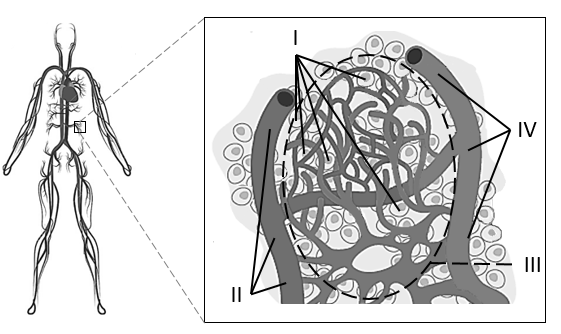
\includegraphics{img/circulatory-system.png}}
\end{center}\vspace*{-0.6cm}
\caption[Visualizaci\'on del sistema circulatorio en el organismo y de la circulaci\'on interna de un tejido]{Visualizaci\'on del sistema circulatorio en el organismo y de la circulaci\'on interna de un tejido. El sistema circulatorio es el encargado de conducir y circular la sangre por todo el organismo y la linfa unidireccionalmente hacia el coraz\'on. En la ampliaci\'on se aprecia el flujo de la circulaci\'on interna del tejido conformado por las c\'elulas~(\emph{I}) y sigue el siguiente recorrido: las arterias~(\emph{II}) traen la sangre oxigenada desde el coraz\'on, pasa por las arteriolas, capilares sangu\'ineos y v\'enulas~(\emph{III}) y finalmente desemboca en las venas~(\emph{IV}) que llevan la sangre de vuelta al coraz\'on para ser oxigenada nuevamente.}
\label{fig-circulatory}

\begin{center}
\scalebox{0.6}{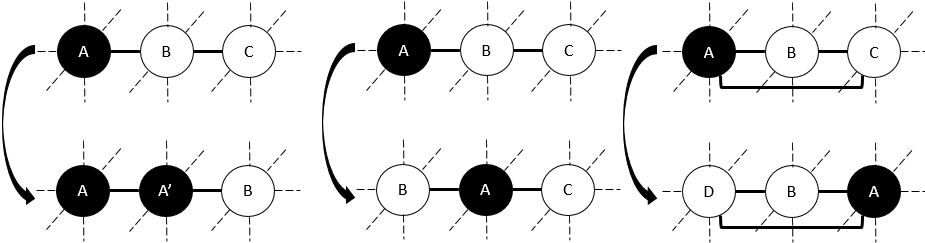
\includegraphics{img/fig-invasion.png}}
\end{center}\vspace*{-0.6cm}
\caption[Representaci\'on de las posibles interacciones entre c\'elulas cancer\'igenas y normales]{Representaci\'on de las posibles interacciones entre c\'elulas cancer\'igenas y normales.\newline
\textbf{Izquierda}: \textit{Divisi\'on Celular} - La c\'elula cancer\'igena A tiene una conexi\'on f\'isica con la c\'elula normal B. En el siguiente instante de tiempo, la c\'elula A se divide dando origen a la c\'elula cancer\'igena A' que pasa a ocupar la posici\'on de B, desplaz\'andola de la misma.\newline
\textbf{Centro}: \textit{Migraci\'on} - La c\'elula cancer\'igena A posee una mutaci\'on que le hace ganar movilidad y la posibilidad de migrar a trav\'es del tejido circundante, que le permite ocupar la posici\'on de la c\'elula normal B. En el siguiente instante de tiempo A se desplaza de su posici\'on, migra hacia B y la desplaza de su posici\'on, ocupando entonces la localizaci\'on de A.\newline
\textbf{Derecha}: \textit{Met\'astasis} - La c\'elula cancer\'igena A posee una conexi\'on distante con la c\'elula normal C, mediante su capacidad de penetrar el sistema circulatorio y abandonarlo en la posici\'on de C. En el siguiente instante de tiempo A se desplaza de su posici\'on, migra hacia C y la desplaza de su posici\'on. La localizaci\'on inicial de A es ocupada por una c\'elula normal D, descendiente de las c\'elulas vecinas de esa posici\'on.}
\label{fig-invasion}
\end{figure}

El conjunto de c\'elulas interconectadas se representa mediante una red, definida a partir de un grafo no dirigido con aristas entre vecinos inmediatos, correspondientes con el primer tipo de conexi\'on, y aristas entre v\'ertices distantes, correspondientes con el segundo tipo de conexi\'on.

\begin{definition}
\label{def-graph}
Sea $G(V, A)$ un grafo no dirigido donde los conjuntos $V$ y $A$ representan los v\'ertices y las aristas del grafo respectivamente. Se usa $V(G)$ y $A(G)$ para denotar los conjuntos de v\'ertices y aristas del grafo $G$ cuando dicho grafo no se enuncia en el contexto.
\end{definition}

\begin{definition}
\label{def-vertex-partition}
El conjunto de v\'ertices $V(G)$ est\'a dividido en dos subconjuntos $V_1(G)$ y $V_2(G)$ disjuntos que forman una partici\'on. Por tanto, satisfacen las siguientes propiedades: 
\begin{subequations}
\begin{equation}
V_1(G) \cup V_2(G) = V(G),
\end{equation}
\begin{equation}
V_1(G) \cap V_2(G) = \emptyset.
\end{equation}
\end{subequations}
\end{definition}

Los subconjuntos que se definen en~\ref{def-vertex-partition} se refieren a 'órganos', también conocidos como localizaciones. Estos órganos corresponden con el órgano primario donde se origina el cáncer y un órgano preferente de metástasis, es decir, un órgano que es comúnmente colonizado por el tipo de cáncer que surgió en el órgano primario. Es importante destacar que estas localizaciones pueden referirse al mismo órgano pero a dos porciones distintas de tejido. Para indicar el subconjunto al que pertenece v\'ertice $v$ determinado se utiliza la notaci\'on $V_v(G)$.

\begin{definition}
\label{def-edge-partition}
Los conjuntos $A^n(G)$ y $A^d(G)$ agrupan las aristas del grafo que corresponden a conexiones inmediatas y distantes respectivamente. Estos conjuntos cumplen con las siguientes propiedades:
\begin{subequations}
\begin{equation}
A^n(G) \cup A^d(G) = A(G),
\end{equation}
\begin{equation}
A^n(G) \cap A^d(G) = \emptyset.
\end{equation}
\end{subequations}
Estas propiedades indican que los subconjuntos de aristas $A^n(G)$ y $A^d(G)$ constituyen una partición del conjunto de aristas $A(G)$.
\end{definition}

En base a los conjuntos de vértices $V(G)$ y de aristas $A(G)$,se definen los elementos representativos $\mathcal{L}$ y $\mathcal{N}$ del modelo de autómatas celulares de la siguiente manera:

\begin{definition} 
    \label{def-L}
El conjunto de c\'elulas $\mathcal{L}$ se define a partir del conjunto de v\'ertices del grafo  $V(G)$:
\begin{align}
\boxed{\mathcal{L} = V(G)}~. \label{eq-L}
\end{align}
\end{definition}

Con el objetivo de evitar ambig\"uedades y sin p\'erdida de rigor, cuando se vaya a referir al conjunto de c\'elulas siempre se utiliza el conjunto de v\'ertices $V(G)$. Los t\'erminos v\'ertice y c\'elula se utilizar\'an indistintamente. 

\begin{definition} 
\label{def-N}
La funci\'on de vecindad $\mathcal{N}$ se define a partir del conjunto de aristas del grafo $A(G)$ como se muestra a continuaci\'on:
\begin{subequations}
\begin{equation}
\boxed{\mathcal{N} : V(G) \times V(G) \rightarrow \lbrace 0,1 \rbrace}~, \label{eq-N}
\end{equation}
\begin{equation}
\boxed{\mathcal{N}(v,w) = \left\lbrace
	\begin{array}{lr}
		0& \textit{si } \lbrace v,w \rbrace \notin A(G)\\
		1& \textit{si } \lbrace v,w \rbrace \in A(G)
	\end{array}
\right.}~, \label{eq-N-2}
\end{equation}
\end{subequations}
o sea, los v\'ertices $v \in V(G)$ Y $w \in V(G)$  son vecinos en el aut\'omata celular si existe una arista en $G$ que los conecta.
\end{definition}

\begin{definition}
\label{def-neighbourhood}
Se define a partir de la funci\'on de vecindad $\mathcal{N}(v,w)$ la vecindad del v\'ertice $v \in V(G)$ como el conjunto de v\'ertices $\mathcal{N}(v)$ que poseen aristas con el v\'ertice $v$, es decir:
\begin{align} 
\mathcal{N}(v) = \lbrace w~|~\mathcal{N}(v,w)=1 \rbrace. \label{eq-neighbourhood}
\end{align}
\end{definition}

\begin{definition}
\label{def-neighbourhoods}
Se define a partir del conjunto $\mathcal{N}(v)$ que contiene a los v\'ertices vecinos de $v$ los subconjuntos $\mathcal{N}^{n}(v) \subseteq \mathcal{N}(v)$ y $\mathcal{N}^{d}(v) \subseteq \mathcal{N}(v)$ que contienen los v\'ertices vecinos inmediatos y los v\'ertices vecinos distantes del v\'ertice $v$ respectivamente:
\begin{subequations}
\begin{equation}
\mathcal{N}^{n}(v) = \lbrace w~|~w \in \mathcal{N}(v) \wedge \lbrace v,w \rbrace \in A^n(G) \rbrace, \label{eq-neighbourhoods}
\end{equation}
\begin{equation}
\mathcal{N}^{d}(v) = \lbrace w~|~w \in \mathcal{N}(v) \wedge \lbrace v,w \rbrace \in A^d(G) \rbrace, \label{eq-neighbourhoods-2}
\end{equation}
\end{subequations}
\end{definition}

\section{Conjunto de c\'elulas: modelo Watts-Strogatz}

En el estudio presentado, se define un tejido blando como un conjunto de células que presenta dos tipos de conexiones: entre células vecinas cercanas y entre células distantes. Para representar estos tipos de conexiones, se utiliza un modelo de autómatas celulares basado en una red de grafos. En~\cite{9}, Duncan J. Watts Y Steven H. Strogatz mostraron que existen muchas redes biol´ogicas, tecnol´ogicas y sociales que yacen entre las redes regulares y las aleatorias que tradicionalmente han sido utilizadas para modelar distintos tipos de sistemas din\'amicos. La clasificaci\'on y diferenciaci\'on de estas redes se lleva a cabo mediante los valores del coeficiente de agrupamiento~(\emph{clustering coefficient}) y la longitud promedio del camino~(\emph{average path length}). 

\begin{definition} 
\label{def-clustering}
Sea $v$ un v\'ertice del grafo que posee $k_v$ aristas que lo conectan a $k_v$ v\'ertices. El valor entre el n\'umero de aristas $K_v$ que existen en realidad entre estos $k_v$ v\'ertices y el n\'umero m\'aximo de aristas posibles\footnote{El n\'umero m\'aximo de aristas posibles se alcanza cuando los $k_v$ vecinos del v\'ertice $v$ pertenecen a un clique. Un clique en un grafo no dirigido es un conjunto de v\'ertices tal que para todo par de v\'ertices, existe una arista que los conecta.} $k_v(k_v-1)/2$ es el coeficiente de agrupamiento del v\'ertice $v$ y se determina como~\cite{7}:
\begin{align}
C_v = \displaystyle\frac{2K_v}{k_v(k_v-1)}. \label{eq-clustering}
\end{align}
\end{definition}

\begin{definition}
\label{def-global-clustering}
El coeficiente de agrupamiento global del grafo $C_G$ es el promedio de todos los coeficientes de agrupamiento individuales $C_v$, es decir~\cite{7}:
\begin{align}
C_G = \displaystyle\frac{1}{|V(G)|}\sum _{v=1} ^{|V(G)|} C_v. \label{eq-global-clustering}
\end{align}
\end{definition}

Si examinamos la figura~\ref{fig-circulatory}, podemos ver que las células que componen el tejido están conectadas con muchas células vecinas inmediatas, que a su vez están conectadas entre sí. De acuerdo con la ecuación que determina el coeficiente de agrupamiento~(\ref{eq-clustering}), y teniendo en cuenta la elevada interconectividad existente, podemos concluir que la mayoría de las células que componen el tejido tienen un alto coeficiente de agrupamiento. Por lo tanto, el coeficiente de agrupamiento global~(\ref{eq-global-clustering}) de la red también tiene un valor alto

En un grafo, la distancia entre dos v\'ertices es el menor n\'umero de aristas de un camino entre ellos. La longitud promedio del camino es la media de las distancias entre todo par de v\'ertices pertenecientes al grafo y se denota como $\ell_G$. Se observa que debido a la existencia de numerosas conexiones distantes a través del sistema circulatorio, la longitud promedio del camino en la red de células es relativamente pequeña.

Por tanto, se hipotetiza que un tejido vivo posee un alto coeficiente de agrupamiento y una pequeña longitud promedio del camino. Estas características son propias de las redes de mundo pequeño, por lo que se utilizan para representar un tejido vivo. Para generar redes de mundo pequeño con estas características, se utiliza el modelo de Watts y Strogatz~\cite{9}. Los autores proponen un modelo de un solo par\'ametro que devuelve una red de mundo peque\~no, ubicada entre un grafo regular y un grafo aleatorio. El algoritmo propuesto por el modelo, que es utilizado para generar las redes de mundo peque\~no usadas en el presente trabajo, es el siguiente~\cite{complexnetworks}:

\begin{enumerate}
\item [(1)] \emph{Inicio:} Comenzamos con un grafo con $q$ v\'ertices, e.g. un anillo o una malla, en los que cada v\'ertice est\'a conectado a $k$ vecinos inmediatos. 

\item [(2)] \emph{Aleatorizaci\'on:} Reconectamos de forma aleatoria cada arista del grafo con una probabilidad $p$ de tal forma que no existan aristas duplicadas ni bucles. Este procedimiento introduce $\frac{p\,*\,q\,*\,k}{2} $ aristas que conectan v\'ertices distantes. Mediante la variaci\'on de $p$, se puede observar la transici\'on entre el orden con $p = 0$ y un grafo totalmente aleatorio con $p = 1$~(Fig.~\ref{fig-relations}).
\end{enumerate}

\begin{figure}[!ht]
\begin{center}
\scalebox{0.6}{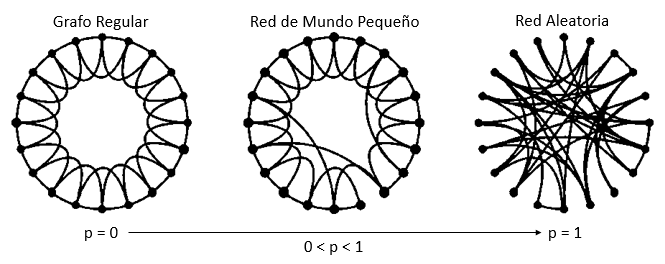
\includegraphics{img/fig-relations.png}}
\end{center}\vspace*{-0.6cm}
\caption[Proceso de reconexi\'on aleatoria del modelo Wattz-Strogatz]{Proceso de reconexi\'on aleatoria del modelo Wattz-Strogatz~(Figura tomada de~\cite{complexnetworks}). Se fijan $q = 20$ v\'ertices, cada uno conectado a sus cuatro vecinos m\'as cercanos. Para $p = 0$ el anillo original se queda inalterado, y a medida que se incrementa $p$ la red se vuelve desordenada. Para $p = 1$ todas las aristas del grafo son reconectadas.}
\label{fig-relations}
\end{figure}

\subsection{Implementaci\'on del modelo Watts-Strogatz}
\label{subsec-watts-2}
El modelo Watts-Strogatz, teniendo en cuenta la hipótesis XII para representar el tejido, comienza con un grafo en el que cada vértice está conectado a un número de sus vecinos inmediatos. Las aristas que forman el grafo son sometidas a un proceso de reconexión, donde se cambia uno de los extremos de la arista. El nuevo extremo se selecciona de manera aleatoria entre los vértices restantes del grafo. Para el proceso de construcción, se considera una cuadrícula que divide el plano en secciones iguales, donde cada celda corresponde a un vértice del grafo (Fig.~\ref{fig-grid-2D-initial}). (revisar poner una imagen de 3d)

\begin{figure}[!ht]
\begin{center}
\scalebox{0.7}{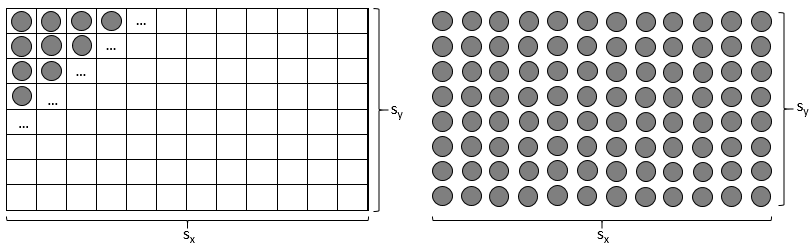
\includegraphics{img/fig-grid-2D-initial.png}}
\end{center}\vspace*{-0.6cm}
\caption[Disposici\'on espacial de los v\'ertices del grafo]{Disposici\'on espacial de los v\'ertices del grafo determinados mediante la cuadr\'icula que se muestra en la imagen izquierda, y que divide el plano en partes iguales para un total de $q = s_x \times s_y = 12 \times 8 = 96$ v\'ertices como se muestra en la imagen derecha.}
\label{fig-grid-2D-initial}
\end{figure}

Como se explicó en la definición~\ref{def-neighbourhoods}, este modelo de autómatas celulares emplea los conjuntos de aristas del grafo $A^n(G)$ y $A^d(G)$ , que representan conexiones inmediatas y distantes, respectivamente. La idea central del modelo Watts-Strogatz para la construcción del grafo es agregar todas las aristas inmediatas al conjunto $A^n(G)$, y a medida que sean reconectadas, son eliminadas de este conjunto y añadidas a $A^d(G)$. Hay diversas opciones para seleccionar las conexiones inmediatas de cada vértice, y cada una de ellas tiene un impacto significativo en las propiedades de la red. En la Figura~\ref{fig-neighbour} se pueden observar algunos ejemplos de posibles configuraciones de vecindad. Inicialmente, definimos la distancia euclidiana para luego establecer una función que permite identificar la vecindad inmediata de un vértice
 
\begin{definition}
\label{def-euclidean-distance}
La funci\'on $d_E(v,w)$, que recibe dos v\'ertices $v \in V(G)$ y $w \in V(G)$, se corresponde con la distancia euclidiana entre los dos puntos del espacio que ocupan dichos v\'ertices y se determina como:
\begin{equation}
d_E(v,w)=\sqrt{(v_x-w_x)^2 + (v_y-w_y)^2}.
\end{equation}
\end{definition}

\begin{definition}
\label{def-neighbourhood-template}
Dado un v\'ertice $v$ en el sistema de coordenadas cartesianas que se utiliz\'o para crear la malla original, definimos como vecindad inmediata de $v$ al conjunto de v\'ertices $\mathcal{N}_I(v,R) = \lbrace w_1, w_2, \ldots, w_m \rbrace$ con $m=|\mathcal{N}_I(v,R)|$ que cumplen la condici\'on $d_E(v,w) \leq R$, es decir:
\begin{equation}
\mathcal{N}_I(v,R) = \lbrace w | d_E(v,w) \leq R \rbrace.
\end{equation}
\end{definition} 

\begin{figure}[!ht]
\begin{center}
\scalebox{0.5}{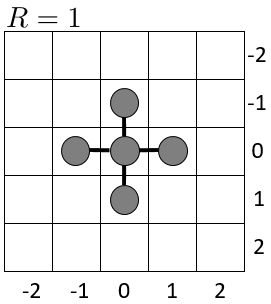
\includegraphics{img/fig-neighbour-R-1.png}}
\scalebox{0.5}{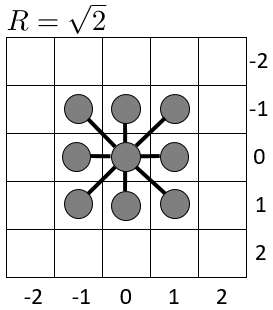
\includegraphics{img/fig-neighbour-R-sqrt(2).png}}
\scalebox{0.5}{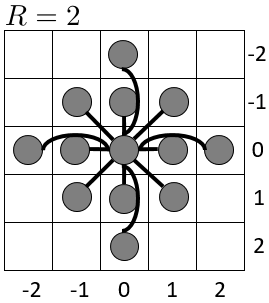
\includegraphics{img/fig-neighbour-R-2.png}}
\scalebox{0.5}{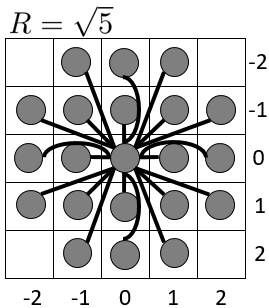
\includegraphics{img/fig-neighbour-R-sqrt(5).png}}
\end{center}\vspace*{-0.6cm}
\caption[Configuraciones de vecindad obtenidas mediante la variaci\'on de $R$]{Configuraciones de vecindad obtenidas mediante la variaci\'on de $R$. En todos los diagramas el v\'ertice $v=(0,0)$ es el centro de la configuraci\'on y se muestra en cada uno el valor de $R$ utilizado para generarla.}
\label{fig-neighbour}
\end{figure}

La inclusi\'on de aristas peri\'odicas al grafo constituye la implementaci\'on de una frontera peri\'odica en la malla, pues esta conecta dos extremos opuestos de la malla. El modelo Watts-Strogatz garantiza que el grafo generado tenga las características especificadas si todos los vértices tienen el mismo grado. Sin embargo, como se puede observar, un vértice que pertenece a uno o varios lados del plano definido tendrá menos aristas. Para solucionar esto, es necesario incluir aristas periódicas, permitiendo que estos vértices tengan el grado correcto. Aunque este método funciona, presenta la desventaja de que el modelo de autómata celulares presentado en este documento no proporciona una interpretación natural de estas aristas periódicas. Se deduce que la adición de estas aristas al grafo afecta sus propiedades.

La selecci\'on de un valor adecuado de $R$, la probabilidad de reconexi\'on $p$ y la inclusi\'on de aristas peri\'odicas son los factores que determinan las propiedades del grafo resultante, cuestiones que se abordan en la secci\'on~\ref{subsec-R-periodic}. Finalmente, la implementaci\'on del modelo Watts-Strogatz se expone en el algoritmo~\ref{alg-watts} y los procedimientos que se llevan a cabo se detallan a continuaci\'on para mayor claridad.

\begin{algorithm}[!ht]
\caption{Implementaci\'on del Modelo Watts-Strogatz.} \label{alg-watts}
\KwData{$s_x, s_y, s_o, p, R$}
\KwResult{$G$}
$V_1=\lbrace \rbrace$\;
$V_2=\lbrace \rbrace$\;
$A^n=\lbrace \rbrace$\;
$A^d=\lbrace \rbrace$\;
\For{$i=0,1,\ldots,s_x-1$}{
	\For{$j=0,1,\ldots,s_y-1$}{
		$v=(i,j)$\;
		\eIf{$i < s_o$}{
			$V_1 = V_1 \cup v $\;}{
			$V_2 = V_2 \cup v $\;}}}
$V=V_1 \cup V_2$\;
\For{$v \in V$}{
	\For{$w \in N_I(v,R)$}{
		$a=\lbrace v,w \rbrace$\;
		$A^n=A^n \cup \lbrace a \rbrace$\;}}
\For{$\lbrace v,w \rbrace \in A^n$}{
	\If{$Random(0,1)<p$}{
		$A^n = A^n \setminus \lbrace v,w \rbrace$\;
		\Repeat{$\lbrace v,w' \rbrace \notin A^n \wedge \lbrace v,w' \rbrace \notin A^d \wedge v \neq w'$}
			{$w'=Select$-$Random$-$Vertex(V)$\;}
		$A^d = A^d \cup \lbrace v,w' \rbrace$\;}}
$A=A^n \cup A^d$\;
$G=(V,A)$\;
\Return $G$\;
\end{algorithm}

\paragraph{Declaraci\'on de los conjuntos que componen el grafo $G$ ($1$-$4$):} Se declaran los conjuntos $V_1$, $V_2$, $A_n$ y $A_d$, inicialmente vac\'ios, correspondientes con los v\'ertices de las localizaciones primaria y secundaria, y las conexiones inmediatas y distantes respectivamente. 

\paragraph{Crear v\'ertices ($5$-$11$):} Se a\~naden a los conjuntos $V_1$ y $V_2$ los v\'ertices que conforman el grafo. Cada v\'ertice $v$ de coordenadas $(v_x,v_y, v_z)$ se corresponde con una celda de la malla. Los valores $s_x$, $s_y$ y $s_z$ son las cantidades de v\'ertices del grafo por cada una de las componentes del plano respectivamente~(Fig.~\ref{fig-grid-2D-initial}). Cada v\'ertice se a\~nade al conjunto $V_1$ o $V_2$ correspondiente, que se determina a partir del par\'ametro $s_o$ con $0 \leq s_o < s_x$ que indica la divisi\'on del grafo entre una localizaci\'on y la otra. 

\paragraph{A\~nadir aristas inmediatas ($12$-$16$):} Se itera por todos los v\'ertices del grafo resultado de la uni\'on de los conjuntos $V_1$ y $V_2$. Por cada v\'ertice $v \in V$ se obtiene su vecindad inmediata $N_I(v,R)$ y se itera por todos los v\'ertices vecinos. Se crea una arista entre $v$ y cada v\'ertice vecino $w$ y se a\~nade al conjunto de aristas inmediatas $A^n$. Dado que la uni\'on entre conjuntos da como resultado un conjunto donde no existen elementos repetidos, no es necesario verificar si una nueva arista ya pertenece al conjunto $A^n$ antes de ser a\~nadida.

\paragraph{Reconexi\'on de las aristas ($17$-$26$):} Se itera por cada arista $a$ del grafo y con probabilidad $p$ se reconecta el v\'ertice destino de la arista. La generaci\'on del valor aleatorio que se compara con $p$ para el c\'alculo de la probabilidad sigue una distribuci\'on uniforme en $(0,1)$. La arista $\lbrace v,w \rbrace$ seleccionada para su reconexi\'on se elimina del conjunto $A^n$ y se procede a encontrar el nuevo v\'ertice destino. El nuevo v\'ertice destino $w'$ se elige de entre todos los v\'ertices del grafo, pero no puede ser el origen de la arista porque no se permiten bucles, y la nueva arista formada no puede existir en el grafo ya que no se permiten duplicados. La nueva arista $\lbrace v,w' \rbrace$ se a\~nade al conjunto $A^d$, identificando satisfactoriamente la nueva conexi\'on como distante. Finalmente, se realiza la uni\'on de los conjuntos $A^n$ y $A^d$, y se declara el grafo $G$ que se retorna como resultado del algoritmo. En la figura~\ref{fig-grid-2D-reconected} se puede apreciar la disposici\'on de los v\'ertices de las caras externas y las conexiones distantes una vez concluido el procedimiento.

\begin{figure}[!ht]
\begin{center}
\scalebox{0.65}{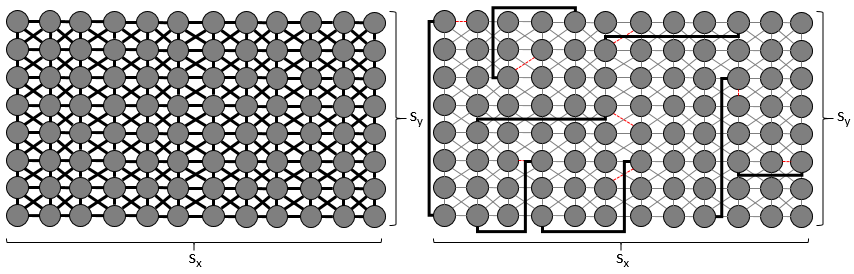
\includegraphics{img/fig-grid-2D-reconected.png}}
\end{center}\vspace*{-0.6cm}
\caption[Detalles de la disposici\'on de las aristas inmediatas y reconectadas en el grafo]{Detalles de la disposici\'on de las aristas inmediatas y reconectadas en el grafo presentado en la figura~\ref{fig-grid-2D-initial}. En el diagrama izquierdo se muestra el grafo construido utilizando la configuraci\'on de vecindad generada con $R=2$, y en el derecho se muestra el grafo una vez concluido el proceso de reconexi\'on de las aristas.}
\label{fig-grid-2D-reconected}
\end{figure}

\subsection{Propiedades del grafo resultante del modelo Watts-Strogatz}
\label{subsec-R-periodic}
En esta sección, proponemos analizar estadísticamente cómo influye la ausencia o presencia de estas aristas en conjunto con varios valores de $R$ en el coeficiente de agrupamiento global de la red y la longitud promedio del camino. El algoritmo~\ref{alg-watts} puede alternar entre la inclusión o exclusión de las aristas periódicas para llevar a cabo esta prueba. Si consideramos que la distancia euclidiana entre dos vértices, 
, que se encuentran en extremos opuestos del grafo $v$ y $w$ es igual a $1$~(siendo $R=1$ el menor valor de radio de la vecindad concebido) entonces la arista peri\'odica entre $v$ y $w$ estar\'a contenida en las vecindades inmediatas de estos v\'ertices. La implementación de esta condición permite alternar entre la inclusión o exclusión de aristas periódicas al grafo resultante.

Para verificar el impacto de las distintas configuraciones de vecindad inmediatas y de la inclusi\'on o no de aristas peri\'odicas en los valores del coeficiente de agrupamiento $C_G$ y de la longitud promedio del camino de la red $\ell_G$ se realizaron diversas pruebas mediante la construcci\'on de distintas redes con una cantidad total de $q = s_x \times s_y = 40 \times 20 = 800$ v\'ertices y alternando distintos valores de $R$ y $p$ con la inclusi\'on o no de aristas peri\'odicas. Cada uno de los valores de $C_G$ y $\ell_G$, mostrados en el cuadro~\ref{table-network-data}, fueron obtenidos promediando los resultados provenientes de la realizaci\'on de $30$ ejecuciones. 
\begin{table}[!ht]
\begin{center}
\scalebox{0.9}{\begin{tabular}{|c|c|c|c|c|c|c|c|c|} \hline
\multicolumn{3}{|c|}{\emph{Par\'ametros}} & \multicolumn{6}{|c|}{\emph{Probabilidad de reconexi\'on}} \\\cline{4-9}

\multicolumn{3}{|c|}{} & \multicolumn{1}{|l|}{$p=0~~$} & \multicolumn{1}{|l|}{$p=10^{-4}$} & \multicolumn{1}{|l|}{$p=10^{-3}$} & \multicolumn{1}{|l|}{$p=10^{-2}$} & \multicolumn{1}{|l|}{$p=10^{-1}$} & \multicolumn{1}{|l|}{$p=1~~$} \\\hline

 & \emph{Aristas} & $C_G$ & \multicolumn{1}{|r|}{$0$} & \multicolumn{1}{|r|}{$0$} & \multicolumn{1}{|r|}{$0$.$0001$} & \multicolumn{1}{|r|}{$0$.$0001$} & \multicolumn{1}{|r|}{$0$.$0007$} & \multicolumn{1}{|r|}{$0$.$0007$} \\\cline{3-9}
 
$R=1$ & \emph{peri\'odicas} & $\ell_G$ & \multicolumn{1}{|r|}{$15$} & \multicolumn{1}{|r|}{$14$.$9699$} & \multicolumn{1}{|r|}{$14$.$1113$} & \multicolumn{1}{|r|}{$10$.$2807$} & \multicolumn{1}{|r|}{$6$.$6847$} & \multicolumn{1}{|r|}{$5$.$1387$} \\\cline{2-9}

 & \emph{No aristas} & $C_G$ & \multicolumn{1}{|r|}{$0$} & \multicolumn{1}{|r|}{$0$} & \multicolumn{1}{|r|}{$0$} & \multicolumn{1}{|r|}{$0$} & \multicolumn{1}{|r|}{$0$.$0007$} & \multicolumn{1}{|r|}{$0$.$0042$} \\\cline{3-9}
 
 & \emph{peri\'odicas} & $\ell_G$ & \multicolumn{1}{|r|}{$19$.$975$} & \multicolumn{1}{|r|}{$19$.$8841$} & \multicolumn{1}{|r|}{$17$.$0731$} & \multicolumn{1}{|r|}{$11$.$8948$} & \multicolumn{1}{|r|}{$7$.$0317$} & \multicolumn{1}{|r|}{$5$.$2847$} \\\hline

 & \emph{Aristas} & $C_G$ & \multicolumn{1}{|r|}{$0$.$4284$} & \multicolumn{1}{|r|}{$0$.$4283$} & \multicolumn{1}{|r|}{$0$.$4271$} & \multicolumn{1}{|r|}{$0$.$4151$} & \multicolumn{1}{|r|}{$0$.$3155$} & \multicolumn{1}{|r|}{$0$.$0088$} \\\cline{3-9}
 
$R=\sqrt{2}$ & \emph{peri\'odicas} & $\ell_G$ & \multicolumn{1}{|r|}{$10$.$8165$} & \multicolumn{1}{|r|}{$10$.$6258$} & \multicolumn{1}{|r|}{$9$.$2563$} & \multicolumn{1}{|r|}{$6$.$6914$} & \multicolumn{1}{|r|}{$4$.$4453$} & \multicolumn{1}{|r|}{$3$.$4615$} \\\cline{2-9}

 & \emph{No aristas} & $C_G$ & \multicolumn{1}{|r|}{$0$.$4554$} & \multicolumn{1}{|r|}{$0$.$4554$} & \multicolumn{1}{|r|}{$0$.$4538$} & \multicolumn{1}{|r|}{$0$.$4423$} & \multicolumn{1}{|r|}{$0$.$3334$} & \multicolumn{1}{|r|}{$0$.$0089$} \\\cline{3-9}

 & \emph{peri\'odicas} & $\ell_G$ & \multicolumn{1}{|r|}{$14$.$8229$} & \multicolumn{1}{|r|}{$14$.$664$} & \multicolumn{1}{|r|}{$11$.$3451$} & \multicolumn{1}{|r|}{$7$.$5682$} & \multicolumn{1}{|r|}{$4$.$6398$} & \multicolumn{1}{|r|}{$3$.$5439$} \\\hline
    
 & \emph{Aristas} & $C_G$ & \multicolumn{1}{|r|}{$0$.$4328$} & \multicolumn{1}{|r|}{$0$.$4326$} & \multicolumn{1}{|r|}{$0$.$4228$} & \multicolumn{1}{|r|}{$0$.$4209$} & \multicolumn{1}{|r|}{$0$.$3219$} & \multicolumn{1}{|r|}{$0$.$0137$} \\\cline{3-9}
 
$R=2$ & \emph{peri\'odicas} & $\ell_G$ & \multicolumn{1}{|r|}{$7$.$6976$} & \multicolumn{1}{|r|}{$7$.$4887$} & \multicolumn{1}{|r|}{$6$.$9479$} & \multicolumn{1}{|r|}{$5$.$1801$} & \multicolumn{1}{|r|}{$3$.$6611$} & \multicolumn{1}{|r|}{$2$.$9432$} \\\cline{2-9}

 & \emph{No aristas} & $C_G$ & \multicolumn{1}{|r|}{$0$.$4731$} & \multicolumn{1}{|r|}{$0$.$4729$} & \multicolumn{1}{|r|}{$0$.$4716$} & \multicolumn{1}{|r|}{$0$.$4595$} & \multicolumn{1}{|r|}{$0$.$3506$} & \multicolumn{1}{|r|}{$0$.$0126$} \\\cline{3-9}
 
 & \emph{peri\'odicas} & $\ell_G$ & \multicolumn{1}{|r|}{$10$.$2375$} & \multicolumn{1}{|r|}{$9$.$8962$} & \multicolumn{1}{|r|}{$8$.$5608$} & \multicolumn{1}{|r|}{$5$.$6387$} & \multicolumn{1}{|r|}{$3$.$8089$} & \multicolumn{1}{|r|}{$3$.$0155$} \\\hline

 & \emph{Aristas} & $C_G$ & \multicolumn{1}{|r|}{$0$.$5157$} & \multicolumn{1}{|r|}{$0$.$5155$} & \multicolumn{1}{|r|}{$0$.$5138$} & \multicolumn{1}{|r|}{$0$.$501$} & \multicolumn{1}{|r|}{$0$.$3832$} & \multicolumn{1}{|r|}{$0$.$0235$} \\\cline{3-9}
 
$R=\sqrt{5}$ & \emph{peri\'odicas} & $\ell_G$ & \multicolumn{1}{|r|}{$5$.$9356$} & \multicolumn{1}{|r|}{$5$.$7967$} & \multicolumn{1}{|r|}{$5$.$0588$} & \multicolumn{1}{|r|}{$3$.$9797$} & \multicolumn{1}{|r|}{$3$.$0175$} & \multicolumn{1}{|r|}{$2$.$5704$} \\\cline{2-9}

 & \emph{No aristas} & $C_G$ & \multicolumn{1}{|r|}{$0$.$5697$} & \multicolumn{1}{|r|}{$0$.$5696$} & \multicolumn{1}{|r|}{$0$.$5679$} & \multicolumn{1}{|r|}{$0$.$5526$} & \multicolumn{1}{|r|}{$0$.$4186$} & \multicolumn{1}{|r|}{$0$.$0217$} \\\cline{3-9}

 & \emph{peri\'odicas} & $\ell_G$ & \multicolumn{1}{|r|}{$7$.$9587$} & \multicolumn{1}{|r|}{$7$.$6352$} & \multicolumn{1}{|r|}{$6$.$1198$} & \multicolumn{1}{|r|}{$4$.$2943$} & \multicolumn{1}{|r|}{$3$.$1359$} & \multicolumn{1}{|r|}{$2$.$6226$} \\\hline
\end{tabular}}
\end{center}\vspace*{-0.6cm}
\caption[Datos de las pruebas realizadas para verificar el impacto de las distintas configuraciones de vecindad y de la inclusi\'on de aristas peri\'odicas en las propiedades del grafo]{Datos de las pruebas realizadas para verificar el impacto de las distintas configuraciones de vecindad y de la inclusi\'on de aristas peri\'odicas en los valores del coeficiente de agrupamiento $C_G$ y de la longitud promedio del camino de la red $\ell_G$. }
\label{table-network-data}
\end{table}

Para un mismo valor de $R$ e independientemente si se incluyen o no las aristas peri\'odicas, a medida que aumenta el valor de la probabilidad de reconexi\'on $p$ disminuye el coeficiente de agrupamiento global y disminuye la longitud promedio del camino, observ\'andose la mayor disminuci\'on a medida que $p$ se acerca a $1$. Esto ocurre porque a medida que m\'as aristas inmediatas son reconectadas a v\'ertices distantes es menor la probabilidad de que estos v\'ertices distantes est\'en conectados con los vecinos inmediatos del v\'ertice focal, disminuyendo el valor del coeficiente de agrupamiento del grafo; pero a medida que aparecen m\'as aristas distantes aumenta la probabilidad de que dos v\'ertices aleatorios est\'en conectados a trav\'es de un camino m\'as corto que utilice estas aristas, disminuyendo la longitud promedio del camino.

Adem\'as se cumple para toda combinaci\'on de $R$ y $p$ que la ausencia de aristas peri\'odicas en el grafo hace que la longitud promedio del camino aumente, dado que permiten la existencia de posibles caminos entre v\'ertices distantes que poseen distancias menores que los caminos que no cuentan con dichas aristas. Pero la ausencia de aristas peri\'odicas, salvo para $p=1$, provoca tambi\'en un aumento en el coeficiente de agrupamiento del grafo, dado que los v\'ertices que poseen vecinos conectados por aristas peri\'odicas aportan valores peque\~nos del coeficiente de agrupamiento ya que existen muchos casos donde dichos v\'ertices vecinos no est\'an conectados entre s\'i.

Dado que la presencia de aristas peri\'odicas carece de una interpretaci\'on natural como se mencion\'o en la secci\'on~\ref{subsec-watts-2}, y que no afectan de forma negativa las propiedades deseadas del grafo resultante como se expuso en el texto anterior, se decide no incluirlas. Se elige la configuraci\'on de vecindad generada con $R=\sqrt{2}$ ya que los grafos construidos con este valor poseen coeficientes de agrupamiento altos y longitudes promedio del camino relativamente peque\~nas. Adem\'as constituye la configuraci\'on de vecindad m\'as sencilla que posee las caracter\'isticas mencionadas ya que provee de una interpretaci\'on natural para las conexiones inmediatas correspondientes con la cercan\'ia f\'isica a diferencia de otras vecindades generadas con valores mayores de $R$; e.g. para $R=2$ se tienen v\'ertices vecinos a distancia $2$ del v\'ertice central. En cuanto a la probabilidad de reconexi\'on esta se encuentra entre los valores $p \in \lbrace 10^{-3}, 10^{-2} \rbrace$ en los que ocurre un r\'apido descenso en el valor de la longitud promedio del camino mientras que el coeficiente de agrupamiento se mantiene casi invariante con un valor cercano a $C_G=0$.$45$ para $R=\sqrt{2}$, que si atendemos lo planteado en~\cite{complexnetworks} constituye un valor alto.
%%% Revisar todo el tema de las aristas periodicas
A partir de estudios realizados anteriormente (tesis de darien) se llega a la conclusión de no incluir las aristas periódicas pues carecen de una interpretación natural y no afectan de forma negativa las propiedades deseadas del grafo. %%%%%%%%%

\section{Marching Cubes}

La técnica de Marching Cubes es un algoritmo de gráficos por computadora que se usa para extraer una malla poligonal de una isosuperficie de un campo escalar discreto tridimensional, como lo son los datos de imágenes de tomografías computarizadas (CT) y resonancias magnéticas (MRI) ~\cite{5}. En el contexto de este proyecto, se utiliza para la representación tridimensional de los tumores, proporcionando una visualización detallada y precisa.Ver en Anexo \ref{fig:tumor}

Este algoritmo trabaja procesando las celdas de los datos de volumen (también conocidas como vóxeles), verificando la intersección entre sus respectivas aristas y la isosuperficie. Los valores de cada vértice de las celdas se comparan con un valor isosuperficial dado, y estos vértices se clasifican como "dentro"  o  "fuera" de la isosuperficie. Una vez definido el tipo de intersección, se realiza una aproximación de la isosuperficie contenida en la celda construyendo triángulos~\cite{1}.

La visualización resultante puede proporcionar una comprensión valiosa de cómo se desarrolla y se propaga el cáncer. Al visualizar el crecimiento del tumor en tres dimensiones, los médicos y científicos pueden obtener una mejor comprensión de la evolución del tumor y cómo puede afectar a los tejidos circundantes. Esta información puede ser esencial para el desarrollo de terapias y tratamientos efectivos para el cáncer.

Debido a que es muy costoso representar y aplicar el algoritmo de Marching Cubes para modelos tan realistas que contengan millones de c\'elulas, en este trabajo se lleva a cabo la implementaci\'on de un escalado del modelo que permite reducir el tama\~no de las dimensiones de nuestro modelo original de aut\'omata celular. Para hacer semejante reducci\'on se procede de la siguiente forma:
\begin{itemize}
    \item Se agrupan las c\'elulas por cuadrantes de dimensi\'on proporcionada por el usuario.
    \item Se buscan los estados de todas las c\'elulas pertenecientes al cuadrante.
    \item El cuadrante adoptar\'a el estado que m\'as se repita entre las c\'elulas que pertenezcan al mismo.
    \item Luego de hacer esto por varios cuadrantes, cada uno reducir\'a su tama\~no desde $(n x m x l)$ a $(1 x 1 x 1)$, siendo $n \leq S_{x} ,m \leq S_{y},l \leq S_{z}$. 
\end{itemize}

En resumen, la técnica de Marching Cubes es una herramienta potente para la visualización tridimensional de datos médicos. En el contexto de la investigación del cáncer, puede proporcionar una representación detallada y precisa del crecimiento de los tumores, lo que puede contribuir significativamente a nuestra comprensión de esta enfermedad y al desarrollo de terapias y tratamientos efectivos.\\

section{Conjunto de estados}
\label{subsec-states}
En la teoría de autómata celulares, un estado es un valor numérico asignado inicialmente a cada célula y que puede variar durante la ejecución. En este modelo, el estado representa el tipo de célula biológica presente. Un corte transversal del tejido muestra que está estructurado en capas, cada una con una función específica dentro del órgano (Fig.\ref{fig-structure}). El crecimiento macroscópico de un tumor depende en gran medida de las interacciones progresivas entre la masa de las células cancerígenas y cada una de estas capas de tejidos. En épocas anteriores de la histología, cada capa del tejido se clasificaba como parte del parénquima o del estroma. El parénquima es el tejido que desempeña la función principal de un órgano específico, mientras que las capas de tejido que proporcionan soporte y apoyo al tejido funcional se denominan estroma. Generalmente, el parénquima está compuesto por el epitelio de un órgano. En la sección\ref{subsec-macro} se presentó el desarrollo idealizado de un tumor que se origina en células de tipo epitelial o carcinoma, y su expansión a través de las distintas capas de tejidos. Por lo tanto, inicialmente, se requiere un estado para las células del tejido epitelial.

\begin{figure}[!ht]
\begin{center}
\scalebox{0.6}{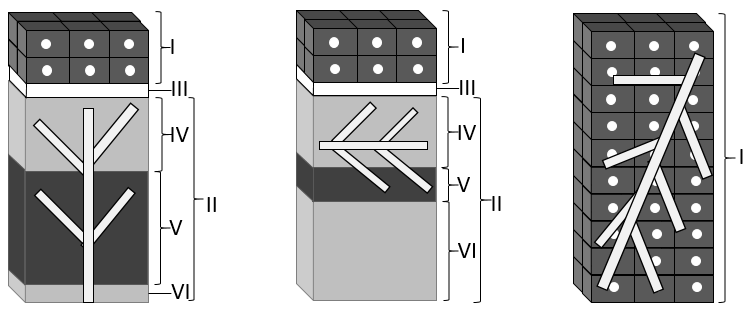
\includegraphics{img/fig-structure.png}}
\end{center}\vspace*{-0.6cm}
\caption[Distribuci\'on de las capas de tejidos en distintos \'organos]{Distribuci\'on de las capas de tejidos en distintos \'organos afectados com\'unmente por el tipo de c\'ancer conocido como carcinoma~\cite{robins}.\newline
\textbf{Izquierda}: \textit{Aparato digestivo} - La estructura mostrada est\'a presente en el es\'ofago, est\'omago, intestinos y recto~\cite{stomach}. Como se puede apreciar todos los tejidos de sost\'en presentan vasculatura. Todas las formas de carcinomas que afectan al aparato digestivo comienzan en la mucosa: carcinoma de c\'elulas escamosas del es\'ofago, adenocarcinoma g\'astrico y adenocarinoma colonrectal. La leyenda se muestra a continuaci\'on: mucosa~(\emph{I}) - formada por epitelio escamoso estratificado en el es\'ofago y por epitelio cil\'indrico columnar en est\'omago e intestinos; estroma~(\emph{II}) - tejidos de sost\'en; membrana basal~(\emph{III}); submucosa~(\emph{IV}) - formada por tejido conjuntivo; muscularis propia~(\emph{V}); serosa~(\emph{VI}).\newline
\textbf{Centro}: \textit{Pulm\'on} - La estructura mostrada est\'a presente en las v\'ias a\'ereas inferiores compuestas por tr\'aquea, bronquios y bronquiolos~\cite{lung}. Como se puede apreciar todos los tejidos de sost\'en con la excepci\'on del cart\'ilago hialino presentan vasculatura. El carcinoma pulmonar de c\'elulas escamosas comienza en la mucosa de los bronquios en la mayor\'ia de los casos. La leyenda se muestra a continuaci\'on: mucosa~(\emph{I}) - formada por epitelio pseudoestratificado columnar en la tr\'aquea y bronquios primarios y por epitelio simple cil\'indrico en los bronquiolos; estroma~(\emph{II}) - tejidos de sost\'en; membrana basal~(\emph{III}); submucosa~(\emph{IV}) - formada por tejido conjuntivo; m\'usculo liso~(\emph{V}); cart\'ilago hialino~(\emph{VI}) - formado por tejido conjuntivo duro.\newline
\textbf{Derecha}: \textit{H\'igado} - El h\'igado est\'a conformado por su propio tipo de c\'elula: los hepatocitos~(\emph{I}) y constituyen su par\'enquima~\cite{liver}. Los vasos del sistema circulatorio est\'an presentes a lo largo del \'organo. El c\'ancer de h\'igado que surge en esta clase de c\'elulas se considera como un carcinoma y se conoce como hepatocarcinoma, aunque las met\'astasis en el h\'igado de otros tipos de c\'ancer son mucho m\'as frecuentes que los que comienzan en el propio \'organo.}
\label{fig-structure}
\end{figure}

Se ha avanzado en el conocimiento de las interacciones complejas entre el tumor y el tejido saludable del cuerpo humano, particularmente aquellas que dan lugar a los comportamientos invasivos y migratorios del cáncer. Sin embargo, aún existen muchos mecanismos que no se comprenden completamente o que son completamente desconocidos hasta la fecha~\cite{kansal3}. A pesar de esto, se pueden identificar varios procesos que contribuyen a la invasión y migración: la degradación de la membrana basal que ocurre durante la angiogénesis, la deformación y movimiento del estroma debido a las fuerzas generadas por la expansión del tumor y la degradación de la matriz extracelular~\cite{kansal3}. El tipo de célula cancerosa que entra en contacto con el estroma determina qué proceso se llevará a cabo. La invasión es llevada a cabo por células cancerosas que pertenecen a la masa del tumor una vez que se ha degradado la membrana basal, y la migración por células cancerosas que poseen las mutaciones para moverse a través del estroma mediante la degradación de la ECM.

A pesar de la variedad de tejidos que componen el estroma, las interacciones entre todos los tejidos de sostén y las células cancerosas conducen a uno de estos dos procesos: invasión o migración. Por lo tanto, no es necesario diferenciar entre las distintas capas de tejidos de sostén en el autómata celular si solo se consideran estas interacciones fundamentales. Posteriormente, se introduce una nueva hipótesis en el modelo que simplifica la dinámica del autómata celular, representando los diversos tipos de tejidos de sostén simplemente como estroma. Las células del autómata correspondientes a este tejido se corresponden entonces con células biológicas reales o con clústeres de macromoléculas presentes en la ECM.

\begin{itemize}
\item [{XIII.}] \textbf{Tejidos de sost\'en o estroma}: \emph{Se representa a la totalidad de los tejidos de sost\'en de un \'organo simplemente como estroma debido a que solo se consideran dos interacciones fundamentales entre los tejidos sanos y el c\'ancer: la invasi\'on y la migraci\'on. Por este motivo no es necesario hacer distinciones entre las distintas capas de sost\'en.} \label{XIII}
\end{itemize}

El tejido epitelial, que es el revestimiento de todas las superficies del cuerpo humano que tienen contacto con el exterior, como los órganos huecos como el estómago y los pulmones, o las estructuras tubulares como los bronquios y las arterias, se conoce como luz de un órgano o lumen, en el caso de los bronquios, arterias e intestinos. En los carcinomas es común que la masa tumoral brote fuera del epitelio, evadiendo los controles de homeostasis del tejido y convirtiéndose en una lesión. La aparición fuera del epitelio constituye un marcador visible del desarrollo neoplásico, por lo que la luz de un órgano o lumen debe ser representada~\cite{robins,stomach,lung,liver,breast}. A partir de lo expuesto anteriormente se inferen los estados para las c'elulas normales. A continuación se define formalmente el estado de una c'elula del aut'omata:

\begin{definition}
\label{def-cellstatus}
Sea un v\'ertice $v \in V(G)$ y un instante de tiempo $n$ del aut\'omata. Se define entonces la funci\'on $s(v,n)$ que devuelve el estado del v\'ertice $v$ en el instante de tiempo $n$:
\begin{subequations}
\begin{equation}
s: V(G) \times \mathbb{N} \rightarrow \mathcal{E}, \label{eq-cellstatus}
\end{equation}
\begin{equation}
s(v,n) = e_i, \label{eq-cellstatus-2}
\end{equation}
\end{subequations}
donde $e_i$ es un estado cualquiera del conjunto de estados $\mathcal{E}$, es decir, $e_i \in \mathcal{E},~\forall i \in \lbrace 0, \ldots, |\mathcal{E}| \rbrace$.
\end{definition}

A continuaci\'on, tomando en cuenta la hip\'otesis XIII sobre los tejidos de sost\'en, se disponen los estados para las c\'elulas normales del aut\'omata:

\begin{itemize}
\item $s(v,n)=0$: El v\'ertice $v$ posee el estado correspondiente con el espacio vac\'io o lumen en el instante de tiempo $n$, y representa las cavidades huecas de los \'organos y conductos.

\item $s(v,n)=1$: El v\'ertice $v$ representa una c\'elula del epitelio en el instante de tiempo $n$, y corresponde con el tejido donde se origina el carcinoma.

\item $s(v,n)=2$: El v\'ertice $v$ posee el estado correspondiente con el estroma en el instante de tiempo $n$, y representa el conjunto de tejidos de sost\'en del \'organo.
\end{itemize}

En cuanto a las c\'elulas cancer\'igenas se distinguen tres estados fundamentales basado en las hip\'otesis del modelo y en lo expuesto en la secci\'on~\ref{sec-cancer}:

\begin{itemize}
\item $s(v,n)=3$: El v\'ertice $v$ representa una c\'elula tumoral en el instante de tiempo $n$, y constituyen la masa neopl\'asica.

\item $s(v,n)=4$: El v\'ertice $v$ representa una c\'elula migratoria en el instante de tiempo $n$, es decir, poseen las mutaciones necesarias para efectuar la cascada metast\'asica.

\item $s(v,n)=5$: El v\'ertice $v$ representa una c\'elula micrometast\'asica en el instante de tiempo $n$, es decir, efectuaron la cascada metast\'a\-sica satisfactoriamente y est\'an colonizando la nueva localizaci\'on, pero pueden ser destruidas por el sistema inmunitario o fallar en dicha colonizaci\'on. 
\end{itemize}

Por ultimo, los estados de las celulas inmunologicas:
\begin{itemize}
    \item $s(v, n) = 6$: El v\'ertice $v$ representa una c\'elula inmune en el instante de tiempo $n$.
    \item $s(v, n) = 7$: El v\'ertice $v$ representa una c\'elula en estado intermedio en el instante de tiempo $n$.
\end{itemize}

Luego el conjunto de estados tiene la forma:
\begin{equation}
\boxed{\mathcal{E} = \lbrace 0, 1, 2, 3, 4, 5, 6, 7 \rbrace}~. \label{eq-states}
\end{equation}

Inicialmente se asigna a cada c\'elula el estado correspondiente a partir de su posici\'on en el tejido de cada localizaci\'on representada en el aut\'omata, es decir, se reproduce la estructura de los tejidos expuestos en la figura~\ref{fig-structure} a partir de la asignaci\'on correspondiente de los distintos estados. A unas pocas c\'elulas del epitelio del \'organo primario se les asigna el estado correspondiente a c\'elulas cancer\'igenas tumorales que forman el foco neopl\'asico inicial. Las transiciones entre los estados de las c\'elulas est\'an sujetas a las reglas de la funci\'on de transici\'on, definidas en las secciones siguientes.

\section{Funci\'on de transici\'on general}
\label{subsec-function}
La dinámica de un autómata se describe mediante una regla de transición local, donde el estado futuro de una célula se deduce de su estado actual y su vecindario. Esta función es espacialmente homogénea, lo que significa que no depende de la ubicación espacial de la célula, aunque puede ser extendida para incluir dependencias temporales o espaciales~\cite{book}. En cuanto a la naturaleza de la regla, esta puede ser determinista o estocástica. En un modelo determinista, la aplicación de la regla a una célula devuelve un único estado en el siguiente instante de tiempo. Por otro lado, en un modelo estocástico, la aplicación de la regla a una célula está condicionada por el valor de una variable aleatoria. Esta variable aleatoria determina la probabilidad de la transición en función del estado anterior de la célula y su vecindario~\cite{book}

Se mencion\'o en la secci\'on introductoria las ventajas de los aut\'omatas celulares para razonar en t\'erminos de individuos, por lo que est\'an mejor ajustados al problema de modelar poblaciones. Sin embargo, el enfoque tradicional en las distintas ramas de la ciencia es utilizar modelos basados en variables continuas, lo que provoca que la inferencia de la funci\'on de transici\'on de estos modelos continuos sea un paso importante a resolver. Comenzamos con las definiciones de configuraci\'on global, configuraci\'on local, funci\'on de transici\'on global y funci\'on de transici\'on local:

\begin{definition}
\label{def-global-conf}
Una configuraci\'on global del aut\'omata $S(n)$~\cite{book} es un vector que contiene los valores de estado de todas las c\'elulas del conjunto $V(G)$ en el instante de tiempo $n$:
\begin{subequations}
\begin{equation}
S(n)=\left(s(v_1,n),s(v_2,n),\ldots,s(v_{|V(G)|},n)\right), \label{eq-global-conf}
\end{equation}
\begin{equation}
S(n)=\left(s(v_i,n)_{v_i \in V(G)}\right). \label{eq-global-conf-2}
\end{equation}
\end{subequations}
El espacio que contiene todas las posibles configuraciones globales del aut\'omata se denota con la letra $\mathcal{S}$ y se define como $\mathcal{S}=\mathcal{E}^{|V(G)|}$. Luego una configuraci\'on global toma uno de los valores posibles del espacio $\mathcal{S}$, o sea $S(n) \in \mathcal{S}$.
\end{definition}

\begin{definition}
\label{def-local-conf}
Una configuraci\'on local del aut\'omata $S(v,n)$~\cite{book} es un vector que contiene los valores de estado de un subconjunto ordenado de c\'elulas del conjunto $V(G)$ en el instante de tiempo $n$.
\begin{equation}
S(v,n)=\left(s(v,n),s(w_1,n),\ldots,s(w_{|\mathcal{N}(v)|},n)\right), \label{eq-local-conf}
\end{equation}
\end{definition}

En el presente trabajo el subconjunto ordenado de c\'elulas est\'a conformado por un v\'ertice focal $v$ y su vecindad $\mathcal{N}(v)$, es decir:
\begin{equation}
S(v,n)=\left(s(v,n),s(w_i,n)_{w_i \in \mathcal{N}(v)}\right). \label{eq-local-conf-2}
\end{equation}

Sin embargo, resulta necesario poder distinguir en una configuraci\'on local los v\'ertices que pertenecen a la vecindad inmediata~(\ref{eq-neighbourhoods}) de los que pertenecen a la vecindad distante~(\ref{eq-neighbourhoods-2}), as\'i como los v\'ertices de cada uno de los \'organos de la red. La implementaci\'on del aut\'omata debe tener en cuenta estas consideraciones.

\begin{definition}
\label{def-local-func}
La funci\'on $\mathcal{R}(S(v,n))$~\cite{book} que recibe una configuraci\'on local $S(v,n)$ centrada en un v\'ertice focal $v$ en el instante de tiempo $n$ y devuelve el estado del v\'ertice $v$ en el siguiente instante de tiempo $n+1$ se denomina funci\'on de transici\'on local. 
\begin{subequations}
\begin{equation}
\boxed{\mathcal{R}:\mathcal{E}^{|\mathcal{N}|} \rightarrow \mathcal{E}}~, \label{eq-local-func}
\end{equation}
\begin{equation}
\boxed{\mathcal{R}(S(v,n)) = \left\lbrace
	\begin{array}{lc}
		e_1& \textit{con probabilidad } \rho(S(v,n) \rightarrow e_1)\\
		e_2& \textit{con probabilidad } \rho(S(v,n) \rightarrow e_2)\\
		\vdots & \ldots\\
		e_{|\mathcal{E}|}& \textit{con probabilidad } \rho(S(v,n) \rightarrow e_{|\mathcal{E}|})
	\end{array}
\right.}~, \label{eq-local-func-2}
\end{equation}
\end{subequations}
donde $e_i \in \mathcal{E},~\forall i \in \lbrace 1,2,\ldots,|\mathcal{E}| \rbrace$, $S(v,n) \in \mathcal{E}^{|\mathcal{N}|}$ y $\rho(S(v,n) \rightarrow e_i)$ es una probabilidad de transici\'on que expresa la posibilidad de llegar al estado elemental $e_i$ a partir de la configuraci\'on local $S(v,n)$. Esta probabilidad de transici\'on satisface las siguientes condiciones:
\begin{subequations}
\begin{equation}
\rho:\mathcal{E}^{|\mathcal{N}|} \times \mathcal{E} \rightarrow [0,1], \label{eq-w} 
\end{equation}
\begin{equation}
\sum_{i=1}^{|\mathcal{E}|}\rho(S(v,n) \rightarrow e_i) = 1. \label{eq-w-sum}
\end{equation}
\end{subequations}
\end{definition}

En un aut\'omata celular estoc\'astico la funci\'on de transici\'on local sigue una distribuci\'on de probabilidad que determina la probabilidad de que cambie el estado actual de una c\'elula de acuerdo a la configuraci\'on de su vecindad. Luego el estado de una c\'elula $v$ en el instante de tiempo $n+1$ se determina a partir de su estado en el instante de tiempo $n$, mediante la aplicaci\'on de la funci\'on de transici\'on local correspondiente.
\begin{equation}
s(v,n+1) = \mathcal{R}(S(v,n)). \label{eq-local-func-3}
\end{equation}

\begin{definition}
\label{def-global-func}
La din\'amica del sistema se define mediante una funci\'on de transici\'on global $\mathcal{R}_g(S(n))$~\cite{book} que recibe una configuraci\'on global del aut\'omata $S(n)$ en el instante de tiempo $n$ y se basa en la aplicaci\'on de la funci\'on de transici\'on local $\mathcal{R}(S(v,n))$ a todas las c\'elulas del aut\'omata para obtener la configuraci\'on global en el siguiente instante de tiempo $n+1$.
\begin{subequations}
\begin{equation}
\mathcal{R}_g:\mathcal{S} \rightarrow \mathcal{S}, \label{eq-global-func}
\end{equation}
\begin{equation}
\mathcal{R}_g(S(n)) = \mathcal{R}(S(v,n)) \quad \forall v \in V(G). \label{eq-global-func-2}
\end{equation}
\end{subequations}
\end{definition}

Luego la evoluci\'on del aut\'omata hacia una configuraci\'on global en el instante de tiempo $n+1$ se determina a partir de la configuraci\'on global en el instante de tiempo $n$, mediante la aplicaci\'on de la funci\'on de transici\'on global.
\begin{equation}
S(n+1) = \mathcal{R}_g(S(n)). \label{eq-global-func-3}
\end{equation}

\subsection{Reglas de la conservaci\'on del estado de las c\'elulas normales y tumorales}
\label{subsec-inert}
El primer conjunto de reglas está vinculado con el comportamiento de las células normales y tumorales definidas en el conjunto de estados del autómata. Según la hipótesis V sobre la invarianza de las células normales, estas permanecen estáticas a lo largo del tiempo. Esto implica que, a menos que exista la presencia de células cancerosas en la vecindad de alguna célula normal, las células normales del autómata mantienen el estado inicial que se les asignó al preparar el modelo para su ejecución. Según la hipótesis IX sobre el proceso de crecimiento simple, una posición ocupada por una célula tumoral permanece ocupada por esta en los instantes de tiempo subsiguientes. Para precisar la funci\'on de transici\'on local de este comportamiento se debe definir una nueva funci\'on $\mathcal{N}_{\mathcal{E'}}^n(S(v,n))$.

\begin{definition}
\label{def-near-neighbours}
La funci\'on $\mathcal{N}_{\mathcal{E'}}^n(S(v,n))$, que recibe una configuraci\'on local $S(v,n)$ en el instante de tiempo $n$ centrada en una c\'elula $v$, devuelve la cantidad de c\'elulas presentes en la vecindad inmediata $\mathcal{N}^{n}(v)$ de dicha configuraci\'on local cuyos estados est\'en contenidos en el subconjunto de estados $\mathcal{E'} = \lbrace e_1, e_2, \ldots , e_{|\mathcal{E'}|}\rbrace \subseteq \mathcal{E}$.
\begin{equation}
\mathcal{N}_{\mathcal{E'}}^n(S(v,n)) = \sum_{\substack{{s(w_i,n) \in S(v,n)}\\{w_i \in \mathcal{N}^{n}(v)}\\{V_{w_i}(G)=V_v(G)}}} \left[\delta(s(w_i,n),e_1) + \delta(s(w_i,n),e_2) + \ldots + \delta(s(w_i,n),e_{|\mathcal{E'}|}) \right], \label{eq-near-neighbours}
\end{equation}
donde se puede apreciar que solo se tienen en cuenta las c\'elulas vecinas inmediatas que pertenecen a la misma localizaci\'on que la c\'elula $v$. 
\end{definition}

\begin{definition}
\label{def-delta}
La funci\'on $\delta(s(w,n),e)$ devuelve el valor $1$ si la c\'elula $w$ posee el estado $e$, $0$ en caso contrario. Formalmente se define como:
\begin{equation}
\delta(s(w,n),e)=\left\lbrace
	\begin{array}{ll}
		1& \textit{si } s(w,n)=e \\
		0& \textit{en caso contrario}
	\end{array}
\right.. 
\end{equation}
\end{definition}

En el caso que el conjunto $\mathcal{E'}$ aparezca en el sub\'indice de la funci\'on $\mathcal{N}_{\mathcal{E'}}^n(S(v,n))$ representado por un solo estado se asume que $\mathcal{E'}$ contiene a ese \'unico estado. Finalmente, la funci\'on de transici\'on local se define a continuaci\'on:
\begin{equation}
s(v,n+1)=\mathcal{R}(S(v,n))=\left\lbrace
	\begin{array}{ll}
		0& \textit{si } s(v,n)=0~\wedge~\mathcal{N}_3^n(S(v,n))=0~\wedge~\mathcal{N}_5^n(S(v,n))=0 \\
		1& \textit{si } s(v,n)=1~\wedge~\mathcal{N}_3^n(S(v,n))=0~\wedge~\mathcal{N}_5^n(S(v,n))=0 \\
		2& \textit{si } s(v,n)=2~\wedge~\mathcal{N}_3^n(S(v,n))=0~\wedge~\mathcal{N}_5^n(S(v,n))=0 \\
		3& \textit{si } s(v,n)=3 
	\end{array}
\right.. \label{eq-inert}
\end{equation}

Estas reglas indican que si el vértice $v$ seleccionado para su actualización es una célula normal en el instante de tiempo $n$, representado por la condición $s(v,n)=e$ en el criterio de selección de la regla, donde $e \in \lbrace 0,1,2 \rbrace$, y no está en presencia de ninguna célula cancerosa que pueda desplazarla de su posición, representado por la condición $\mathcal{N}_3^n(S(v,n))=0~\wedge~\mathcal{N}_5^n(S(v,n))=0$, esta célula mantiene su estado en el instante de tiempo $n+1$. Una célula tumoral mantiene su estado indefinidamente dado por la condición $s(v,n)=3$. En secciones posteriores se exponerán los mecanismos que provocan la aparición de células que presentan los demás estados cancerosos.

La funci\'on $\mathcal{N}_{\mathcal{E'}}^n(S(v,n))$~(\ref{eq-near-neighbours}) solo toma en cuenta las c\'elulas vecinas inmediatas de la c\'elula $v$ que pertenezcan a la misma localizaci\'on que $v$ como se aprecia en la condici\'on $V_{w_i}(G)=V_v(G)$ de la sumatoria. La consideración de que las interacciones entre las células inmediatas están limitadas al interior de cada localización, mientras que la interacción entre localizaciones ocurre a través de las conexiones entre las células distantes, está presente en todas las reglas de transición del autómata. Esto se deriva de la hipótesis XI sobre las vías de la metástasis, que establece que las únicas vías consideradas son las hemáticas y linfáticas, dejando sin examinar las vías intratorácicas, es decir, que la expansión del tumor pueda penetrar de forma directa los órganos cercanos. Por lo tanto, se puede inferir que todas las células pertenecientes a un tumor cualquiera de la simulación pertenecen a una misma localización.

\subsection{Reglas del crecimiento tumoral}
\label{subsec-celldiv}
El conjunto de reglas que se define a lo largo de esta secci\'on se relaciona con el comportamiento de las c\'elulas cancer\'igenas que conforman una masa tumoral. Dicho comportamiento se define a partir de un grupo de suposiciones que determinan la naturaleza macrosc\'opica del tumor as\'i como las interacciones entre las c\'elulas cancer\'igenas y las c\'elulas normales del tejido. Como se expuso en las hip\'otesis I y II sobre la progresi\'on idealizada del desarrollo tumoral y las mutaciones de las c\'elulas cancer\'igenas respectivamente, el desarrollo del tumor se divide en las etapas avascular y vascular, donde en cada etapa se manifiestan determinados comportamientos caracter\'isticos relacionados con la expresi\'on de las mutaciones representativas del c\'ancer. 

En este modelo, se simulan dos tipos de tumores: el primario y los tumores secundarios o metástasis. Ambos tipos de tumores se diferencian en las células cancerosas que los componen, su comportamiento y la influencia de los factores ambientales. Durante la fase vascular, un tumor primario y los tumores metástasis están conformados por células que presentan el mismo grado de mutaciones, por lo que se comportan de la misma manera, ambos son capaces de llevar a cabo la invasi\'on, la migraci\'on y la met\'astasis. Sin embargo, según la hipótesis II durante la fase avascular, un tumor primario solo tiene las mutaciones relacionadas con el ciclo celular, mientras que los tumores secundarios tienen todas las mutaciones características del cáncer, lo que afecta su comportamiento. A su vez, la invasi\'on de un tejido sano se traduce en la capacidad del tumor de desplazar a los distintos tipos de c\'elulas normales correspondientes con estos tejidos de su posici\'on, mediante las fuerzas expansivas causadas por el aumento de la concentraci\'on de c\'elulas cancer\'igenas en el interior del tumor o por su propia descendencia. 

El cáncer representado en el modelo se conoce como carcinoma y tiene su origen en las células epiteliales que revisten los órganos. Un tumor primario se expande dentro del epitelio y hacia el lumen durante la etapa avascular, gracias a la angiogénesis que produce la degradación de la membrana basal y los cambios en la matriz de interacción intercelular. Durante la etapa vascular, la expansión del tumor ocurre en el epitelio y el lumen, y también adquiere la capacidad de invadir el estroma. Por otro lado, una micrometástasis induce la angiogénesis desde el inicio, por lo que puede invadir diferentes tejidos sanos durante la etapa avascular. Aunque la micrometástasis tiene todos los criterios característicos del cáncer, no empieza a expresar los relacionados con la migración y la metástasis hasta la etapa vascular. La invasi\'on de los tejidos de sost\'en de un tumor primario en etapa avascular no tiene que ocurrir exactamente en el momento que se comienza a desarrollar la angiog\'enesis, pero constituye el caso promedio. En cuanto a la influencia de factores externos, una micromet\'astasis puede ser eliminada del aut\'omata por dos causas fundamentales: su destrucci\'on por parte del sistema inmunitario o su incapacidad de sobrevivir en el entorno donde crece, donde ambos factores poseen una estrecha relaci\'on con la teor\'ia de la semilla y el sustrato expuesta en la secci\'on~\ref{subsec-meta}. Se asume que un tumor en etapa vascular, sea primario o secundario, no puede ser eliminado por el sistema inmunitario y que se adapt\'o satisfactoriamente al entorno donde se desarrolla. Con el objetivo de que el aut\'omata represente todo el ciclo vital del c\'ancer, un tumor primario durante la etapa avascular no puede ser eliminado por el sistema inmunitario y posee la capacidad de sobrevivir en su localizaci\'on inicial. Estas caracterizaciones se recogen en el cuadro comparativo~\ref{table-comparison} y el ciclo vital del c\'ancer representado en este modelo se muestra en la figura~\ref{fig-tumor-progresion}. 

\begin{table}[!ht]
\begin{center}
\scalebox{0.9}{\begin{tabular}{|c|c|c|c|c|} \hline
\emph{Caracter\'isticas} & \multicolumn{2}{|c|}{\emph{Tumor primario}} & \multicolumn{2}{|c|}{\emph{Tumor secundario}} \\\cline{2-5}
 & \emph{Avascular} & \emph{Vascular} & \emph{Avascular*} & \emph{Vascular} \\\hline
\emph{Invasi\'on}        & No   & S\'i & S\'i & S\'i \\ \hline
\emph{Migraci\'on}       & No   & S\'i & No   & S\'i \\ \hline
\emph{Met\'astasis }     & No   & S\'i & No   & S\'i \\ \hline
\emph{Supervivencia en el}   & Siempre & Siempre & Existe la    & Siempre     \\ 
\emph{entorno de desarrollo} &         &         & Probabilidad &    \\ \hline
\emph{Destrucci\'on por el}  & Nunca   & Nunca   & Existe la    & Nunca   \\ 
\emph{sistema inmunitario}   &         &         & Probabilidad &      \\ \hline
\end{tabular}}
%\scalebox{0.85}{\includegraphics{img/table-comparison.png}}
\end{center}\vspace*{-0.6cm}
\caption[Comparaci\'on entre los dos tipos de tumores representados tomando en cuenta sus caracter\'isticas durante ambas etapas de su desarrollo]{Comparaci\'on entre los dos tipos de tumores representados tomando en cuenta sus caracter\'isticas durante ambas etapas de su desarrollo. \emph{En el cuadro:} (*) Un tumor secundario en etapa avascular se corresponde con una micromet\'astasis.}
\label{table-comparison}
\end{table}

\begin{figure}[!ht]
\begin{center}
\scalebox{0.8}{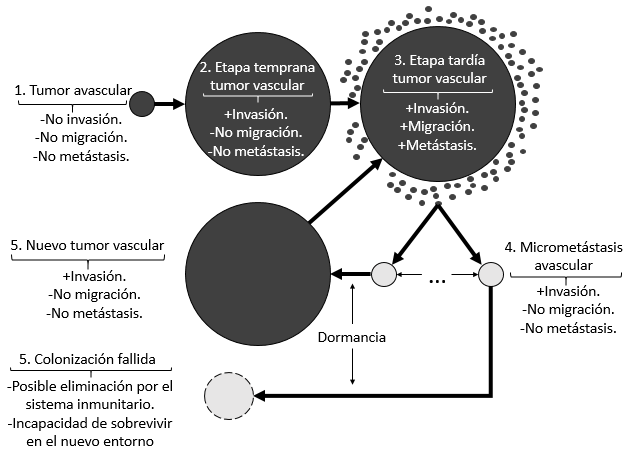
\includegraphics{img/fig-tumor-progresion-2.png}}
\end{center}\vspace*{-0.6cm}
\caption[Ciclo vital del c\'ancer representado por el modelo]{Ciclo vital del c\'ancer representado por el modelo. Como se puede apreciar la \'unica diferencia existente en el modelo entre un tumor primario y uno secundario es su comportamiento durante la etapa avascular, ya que se asume que un tumor primario siempre sobrevive y se desarrolla de forma satisfactoria en su entorno, mientras que una micromet\'astasis puede fallar en colonizar su nuevo entorno o ser destruida por el sistema inmunitario.}
\label{fig-tumor-progresion}
\end{figure}

En la presente secci\'on, referente al surgimiento de c\'elulas tumorales que conforman la masa neopl\'asica, se expone el procedimiento seguido para definir las reglas que reproducen el crecimiento de un tumor primario en ambas etapas y de los tumores secundarios durante la etapa vascular. La transici\'on entre las etapas avascular y vascular en un tumor primario ocurre de forma natural cuando su poblaci\'on celular alcanza cierto punto, mientras que en una met\'astasis esta transici\'on est\'a determinada por un proceso conocido como dormancia o latencia\footnote{De ahora en adelante cuando se utilice la palabra tumor nos estaremos refiriendo a un tumor primario o a un tumor secundario en etapa vascular, salvo que se especifique lo contrario.}. El crecimiento de un tumor secundario durante la etapa avascular y el proceso de dormancia ser\'an expuestas en las secciones~\ref{subsec-micrometastasis} y~\ref{subsec-dormancy}. 

Como se mostr\'o anteriormente la vascularizaci\'on de un tumor es un elemento distintivo de su desarrollo, ya que la difusi\'on de nutrientes permite al propio tumor crecer solo hasta un l\'imite permitido, y es el nuevo suministro de nutrientes proveniente de la neovasculatura la que permite que el tumor contin\'ue su crecimiento m\'as all\'a de dicho l\'imite. Como se mostr\'o en la hip\'otesis VIII sobre el desarrollo tumoral en funci\'on de la poblaci\'on, el modelo asume que la din\'amica de un tumor sigue la funci\'on de crecimiento log\'istico de Verhulst~\cite{verhulst}, presentada a continuaci\'on:
\begin{equation}
\left\lbrace
	\begin{array}{l}		
		\displaystyle\frac{dP}{dt} = rP(1-\displaystyle\frac{P}{K})\vspace*{0.2cm}\\
		P(t=0)=P_0
	\end{array}
\right., \label{eq-verhulst}
\end{equation}
donde se expresa que la variaci\'on de la poblaci\'on respecto al tiempo depende de un ritmo de crecimiento $r$, la poblaci\'on $P$ en ese instante de tiempo y un valor $K$ que representa la capacidad de carga, es decir, la cantidad de individuos de la poblaci\'on que puede sostener el entorno. La angiog\'enesis se puede traducir como un aumento de la capacidad de carga $K$ del entorno, as\'i como un incremento en el ritmo de proliferaci\'on celular debido a que la neovasculatura constituye un m\'etodo de suministro m\'as eficiente que la difusi\'on de nutrientes. Por tanto la din\'amica global del crecimiento ser\'a descrita por dos expresiones: una correspondiente con la etapa avascular y una correspondiente con la etapa vascular, ambas con sus par\'ametros particulares. Como consecuencia del an\'alisis anterior se adopta la siguiente hip\'otesis:

\begin{itemize}
\item [{XIV.}] \textbf{Interpretaci\'on de la neovasculatura}: \emph{Se asume que la neovasculatura que crece en el interior de un tumor producto de la angiog\'enesis produce un aumento en la capacidad de carga del entorno y en el ritmo de proliferaci\'on del propio tumor.} \label{XIV}
\end{itemize} 

En las reglas sobre la conservaci\'on del estado de las c\'elulas normales del aut\'omata~(\ref{eq-inert}) se especific\'o que dichas c\'elulas no cambian de estado salvo que en se encuentren en presencia de c\'elulas cancer\'igenas pertenecientes a alg\'un tumor. Esto significa que la regla del crecimiento tumoral se puede definir a partir de esta condici\'on, es decir, las c\'elulas normales tienen una probabilidad de ser desplazadas de su posici\'on si se encuentran pr\'oximas a una o varias c\'elulas cancer\'igenas pertenecientes a uno o distintos tumores, o en t\'erminos de la funci\'on~(\ref{eq-near-neighbours}) $\mathcal{N}_3^n(S(v,n)) > 0$. Por tanto las reglas se definen de la siguiente forma:
\begin{equation}
s(v,n+1)=\mathcal{R}(S(v,n))=\left\lbrace
	\begin{array}{ll}
		\zeta_0(S(v,n))& \textit{si } s(v,n)=0~\wedge~\mathcal{N}_3^n(S(v,n)) > 0 \\
		\zeta_1(S(v,n))& \textit{si } s(v,n)=1~\wedge~\mathcal{N}_3^n(S(v,n)) > 0 \\
		\zeta_2(S(v,n))& \textit{si } s(v,n)=2~\wedge~\mathcal{N}_3^n(S(v,n)) > 0 
	\end{array}
\right., \label{eq-celldiv}
\end{equation}
donde $\zeta_i(S(v,n)) \in \lbrace i,3 \rbrace$ con $i \in \lbrace 0,1,2 \rbrace$ son variables aleatorias con la siguiente distribuci\'on de probabilidad:
\begin{subequations}
\begin{equation}
P(\zeta_i(S(v,n))=i) = 1 - \rho(S(v,n) \rightarrow 3),
\end{equation}
\begin{equation}
P(\zeta_i(S(v,n))=3) = \rho(S(v,n) \rightarrow 3).
\end{equation}
\end{subequations}

De las expresiones anteriores se infiere que la probabilidad de que una c\'elula normal sea desplazada por una c\'elula cancer\'igena tiene el valor correspondiente con la evaluaci\'on de la probabilidad de transici\'on $\rho(S(v,n) \rightarrow 3)$, mientras que la probabilidad de que permanezca en el estado original es $1-\rho(S(v,n) \rightarrow 3)$. Como un tumor siempre se expande hacia posiciones vecinas ocupadas por c\'elulas normales se puede asegurar que la masa tumoral posee una forma compacta donde cada c\'elula cancer\'igena posee en su vecindad a otras c\'elulas cancer\'igenas, en correspondencia con lo expresado en la hip\'otesis X sobre la adhesi\'on celular. Esta probabilidad de transici\'on, seg\'un la concepci\'on cl\'asica de un aut\'omata celular, debe definirse de forma tal que utilice solamente la informaci\'on de la configuraci\'on local para estimar el valor resultante. En el contexto del presente modelo es necesario que la probabilidad incorpore la informaci\'on relacionada con el modelo de crecimiento log\'istico.

\subsubsection{Proceso de inferencia de la regla}
La visión tradicional de un autómata celular postula que la función de transición local solo puede tomar como entrada la configuración local de la célula $v$ seleccionada para su actualización~\cite{book}. Sin embargo, este enfoque presenta una limitación ya que no permite simular varios procesos biológicos, tecnológicos y sociales en los que las posibles transiciones dependen de información adicional. En~\cite{guinot} se presenta una metodología para inferir reglas estocásticas de un autómata celular a partir de modelos continuos. Esta metodología introduce conceptos que pueden ser utilizados para expandir la concepción clásica. En este modelo, se combina la probabilidad de transición con las diferentes configuraciones locales posibles, es decir, el criterio de selección de la regla que se debe aplicar en cada caso depende del estado de la configuración local, mientras que la probabilidad de transición se obtiene a partir del modelo continuo. La adopción de estas ideas es especialmente beneficiosa ya que la función de transición local y el criterio de selección de la regla a aplicar se mantienen según la definición clásica, y solo se modifica la probabilidad de transición. Los nuevos argumentos de la probabilidad de transición constituyen dependencias heterogéneas de la función de transición que no están concebidas en la concepción clásica de los autómata celulares. Se comienza especificando una probabilidad de transición alternativa que reciba la información relevante del modelo continuo~\cite{guinot}.

\begin{definition}
\label{prop-newlocal-func}
Sea una extensi\'on de la funci\'on de transici\'on local definida en~\ref{def-local-func} que incluye una probabilidad de transici\'on alternativa que depende de nuevos argumentos:
\begin{equation}
s(v,n+1) = \mathcal{R}(S(v,n)) = e_i~~\textit{con probabilidad } \rho(\tau(v,n,N_{tum}) \rightarrow e_i), \label{eq-newlocal-func}
\end{equation}
donde $\tau(v,n,N_{tum})$ es una funci\'on que devuelve el tiempo transcurrido relativo al surgimiento del tumor que intenta expandirse hacia $v$ en el instante de tiempo $n$; e.g. si el instante de tiempo en que surgi\'o el tumor en cuesti\'on es $n'$ el tiempo transcurrido relativo es $n_r = n - n'$. 
\end{definition}

El conjunto $N_{tum}$ contiene la informaci\'on correspondiente con los instantes de tiempo en que surgieron los tumores contenidos en la simulaci\'on. Con el objetivo de ilustrar de forma clara el proceso de inferencia se asume durante esta secci\'on que solo existe un tumor expandi\'endose hacia la c\'elula $v$. En la secci\'on que se muestra a continuaci\'on que trata sobre la inclusi\'on de nuevas hip\'otesis al modelo se esclarece esta suposici\'on exponiendo un m\'etodo de resoluci\'on de las distintas situaciones de competencia que pueden surgir entre varios tumores cuando se expanden hacia una misma c\'elula. En el algoritmo~\ref{alg-n-r} se muestra la implementaci\'on de la funci\'on $\tau(v,n,N_{tum})$ a modo de definici\'on donde se tiene en cuenta la suposici\'on hecha anteriormente, $N^n(v)$ es la funci\'on de vecindad inmediata definida en~\ref{def-neighbourhoods}, la funci\'on $tumor(w)$ devuelve el identificador \'unico asociado al tumor al que pertenece $w$ y la funci\'on $s(w,n)$ es el estado de la c\'elula $w$ en el instante de tiempo $n$ definida en~\ref{def-cellstatus}. Aunque funciones como $\tau(v,n,N_{tum})$ pueden ser definidas matem\'aticamente, se prefiere la definici\'on mediante un algoritmo pues brinda informaci\'on adicional sobre la implementaci\'on del aut\'omata celular.

\begin{algorithm}[!ht]
\caption{Definici\'on de la funci\'on $\tau(v,n,N_{tum})$.} \label{alg-n-r}
\KwData{$v, n, N_{tum}$}
\KwResult{$n_r$}
\For{$w \in N^n(v)$}{
	\If{$s(w,n)=3$}{
		$n_r = n - N_{tum}[tumor(w)]$\;
		\Return $n_r$\;}}
\end{algorithm}

Se reescribe la regla de la aparici\'on de c\'elulas tumorales~(\ref{eq-celldiv}) tomando en cuenta la nueva probabilidad de transici\'on alternativa propuesta en~(\ref{prop-newlocal-func}) como:
\begin{equation}
s(v,n+1)=\mathcal{R}(S(v,n))=\left\lbrace
	\begin{array}{ll}
		\zeta_0(\tau(v,n,N_{tum}))& \textit{si } s(v,n)=0~\wedge~\mathcal{N}_3^n(S(v,n)) > 0 \\
		\zeta_1(\tau(v,n,N_{tum}))& \textit{si } s(v,n)=1~\wedge~\mathcal{N}_3^n(S(v,n)) > 0 \\
		\zeta_2(\tau(v,n,N_{tum}))& \textit{si } s(v,n)=2~\wedge~\mathcal{N}_3^n(S(v,n)) > 0 
	\end{array}
\right., \label{eq-celldiv-2}
\end{equation}
donde la distribuci\'on de probabilidad de las variables aleatorias $\zeta_i(\tau(v,n,N_{tum})) \in \lbrace i,3 \rbrace$ con $i \in \lbrace 0,1,2 \rbrace$ quedar\'ia como:
\begin{subequations}
\begin{equation}
P(\zeta_i(\tau(v,n,N_{tum})=i) = 1 - \rho(\tau(v,n,N_{tum}) \rightarrow 3),
\end{equation}
\begin{equation}
P(\zeta_i(\tau(v,n,N_{tum})=3) = \rho(\tau(v,n,N_{tum}) \rightarrow 3).
\end{equation}
\end{subequations}

El c\'alculo de la probabilidad de transici\'on $\rho(\tau(v,n,N_{tum}) \rightarrow 3)$ se define a partir de la ecuaci\'on de crecimiento log\'istico de Verhulst. Primero se debe escribir la ecuaci\'on de crecimiento de forma tal que podamos expresar la variaci\'on de la poblaci\'on desde un instante de tiempo $n$ hacia el instante $n+1$. Para valores peque\~nos de $\Delta t$, la derivada de la ecuaci\'on de crecimiento se puede determinar de forma aproximada como: 
\begin{subequations}
\begin{equation}
\frac{dP(t)}{dt} \approx \frac{P(t+\Delta t) - P(t)}{\Delta t},
\end{equation}
\begin{equation}
P'(t) \approx \frac{P(t+\Delta t) - P(t)}{\Delta t},
\end{equation}
\begin{equation}
\Delta t P'(t) \approx P(t+\Delta t) - P(t),
\end{equation}
\begin{equation}
P(t+\Delta t) - P(t) \approx \Delta t P'(t),
\end{equation}
\end{subequations}
luego si tomamos el tiempo $t$ como una variable discreta, y hacemos $t=n\Delta t$, obtenemos:
\begin{subequations}
\begin{equation}
P(n\Delta +\Delta t) - P(n\Delta t) \approx \Delta t P'(n\Delta t),
\end{equation}
\begin{equation}
P((n+1)\Delta t) - P(n\Delta t) \approx \Delta t P'(n\Delta t). \label{eq-delta}
\end{equation}
\end{subequations}

La expresi\'on~(\ref{eq-delta}) se interpreta como la variaci\'on de la poblaci\'on del tumor entre los instantes de tiempo $n$ y $n+1$ como se puede apreciar en la parte izquierda $P((n+1)\Delta t) - P(n\Delta t)$. El tiempo que transcurre en el modelo continuo entre los instantes de tiempo $n$ y $n+1$ del aut\'omata celular es $\Delta t$. Se infiere de~(\ref{eq-delta}) que la probabilidad de transici\'on $\rho(\tau(v,n,N_{tum})\rightarrow 3)$ se calcula mediante $P'(t)$. A partir de~(\ref{eq-verhulst}), sujeta a la condici\'on inicial, se obtiene~(ver ap\'endice~\ref{app-a} para el proceso de resoluci\'on):
\begin{equation}
P(t) = \frac{P_0 K}{P_0 + (K-P_0)e^{-rt}}, \label{eq-verhulst-solution}
\end{equation} 
cuya derivada $P'(t)$ finalmente tiene la forma~(ver ap\'endice~\ref{app-b} para el proceso de derivaci\'on):
\begin{equation}
P'(t) = \frac{P_0 K r e^{rt}(K-P_0)}{(P_0 e^{rt} + K - P_0)^2}. \label{eq-prob}
\end{equation}

Se expuso anteriormente que la probabilidad de transici\'on $\rho(\tau(v,n,N_{tum}) \rightarrow 3) \in [0,1]$, lo cual no ocurre con la funci\'on $P'(t)$, por lo que es necesario analizar su imagen. Con este objetivo derivamos la funci\'on $P'(t)$ para buscar los puntos estacionarios~(ver ap\'endice~\ref{app-c} para el proceso de derivaci\'on), obteni\'endose: 
\begin{equation}
P''(t) = \frac{P_0 K r^2 e^{rt} (P_0-K)(P_0 e^{rt} + P_0 - K)}{(P_0 e^{rt} + K - P_0)^3},
\end{equation}
donde se infiere que $P'(t)$ posee un m\'aximo cuando:
\begin{equation}
t = \frac{1}{r} \ln\frac{K-P_0}{P_0}, \label{eq-cond-t}
\end{equation}
evaluando $P'(t)$ en este valor de $t$ obtenemos la probabilidad m\'axima de crecimiento:
\begin{equation}
P'\left(t = \frac{1}{r} \ln\frac{K-P_0}{P_0}\right) = \frac{Kr}{4}.
\end{equation}

Por tanto $P'(t)$ alcanza su valor m\'aximo en el punto $(\frac{1}{r} \ln\frac{K-P_0}{P_0}, \frac{Kr}{4})$, donde este valor depende directamente de la capacidad de carga $K$ y del ritmo de crecimiento $r$, devolviendo el intervalo de probabilidad $[0, \frac{Kr}{4}]$. Supongamos que $\rho_{max}$ es el valor m\'aximo de la funci\'on $P'(t)$ en su dominio, de tal forma que $P'(t) \in [0, \rho_{max}]$ sujeto a la condici\'on $\rho_{max} \leq 1$. Despejando la siguiente desigualdad:
\begin{equation}
\frac{K r}{4} \leq \rho_{max},
\end{equation}
se obtiene la condici\'on necesaria para que la funci\'on $P'(t) \in [0,\rho_{max}]$, quedando:
\begin{equation}
r \leq \frac{4 \rho_{max}}{K}. \label{eq-cond-1}
\end{equation}

Mediante la condici\'on~(\ref{eq-cond-1}) se puede asegurar que la probabilidad de crecimiento tumoral que se obtiene mediante la evaluaci\'on de $P'(t)$ pertenece al intervalo $[0,\rho_{max}]$, permitiendo un mecanismo de ajuste del modelo mediante la adecuada selecci\'on de $\rho_{max}$. Este mecanismo de ajuste se sustenta en el hecho de que los modelos de aut\'omatas que se recogen en trabajos anteriores se dividen en dos clases generales: los que reproducen un modelo concebido espec\'ificamente para la reproducci\'on del crecimiento de tumores como~\cite{ruben}, y los que reproducen un modelo general de crecimiento y lo adaptan al caso espec\'ifico del crecimiento de tumores como~\cite{kansal,kansal3,ruanxiaoca}, categor\'ia a la que pertenece el presente trabajo. En el segundo tipo de trabajos es com\'un encontrar este mecanismo en la forma de una probabilidad base como se aprecia en~\cite{kansal}. La condici\'on~\ref{eq-cond-1} est\'a expresada en base a $r$ dado que el valor de $\rho_{max}$ se selecciona a priori y $K$ se determina directamente a partir de la informaci\'on existente acerca del proceso de crecimiento de un tumor, mientras que el proceso de estimar $r$ carece de una metodolog\'ia por lo que es imprescindible poseer la mayor cantidad de informaci\'on acerca de su valor. Las estimaciones de estos valores se llevan a cabo en la secci\'on~\ref{sec-validation}.

A partir de las hip\'otesis VIII y XIV sobre el desarrollo tumoral en funci\'on de la poblaci\'on y la interpretaci\'on de la neovasculatura respectivamente, se infiere que el crecimiento de la poblaci\'on tumoral se describe mediante dos expresiones correspondientes a las etapas avascular y vascular, cada una con sus valores propios del ritmo de crecimiento $r$ y capacidad de carga $K$. Se puede deducir que ambas etapas poseen tambi\'en valores propios de poblaci\'on inicial $P_0$, donde la poblaci\'on inicial de la etapa vascular $P_0^v$ se corresponde con la capacidad de carga del entorno durante la etapa avascular $K_a$, es decir, $K_a = P_0^v$. An\'alogamente se pueden definir a priori valores de probabilidad m\'aximos $\rho_{max}$ para cada una de estas etapas. Finalmente las probabilidades de transici\'on, con $t=n\Delta t$, quedar\'ian como:
\begin{subequations}
\begin{equation}
\rho_a(n\Delta t) = \displaystyle\frac{P_0^a K_a r_a e^{r_a n\Delta t}(K_a-P_0^a)}{(P_0^a e^{r_a n\Delta t} + K_a - P_0^a)^2},
\label{eq-pa}
\end{equation}
\begin{equation}
\rho_v(n\Delta t) = \displaystyle\frac{P_0^v K_v r_v e^{r_v n\Delta t}(K_v-P_0^v)}{(P_0^v e^{r_v n\Delta t} + K_v - P_0^v)^2}.
\label{eq-pv}
\end{equation}
\end{subequations}

Utilizando las expresiones~(\ref{eq-pa},~\ref{eq-pv}) y diferenciando las etapas del desarrollo tumoral en base a un nuevo par\'ametro $n_a$ que indica el per\'iodo de tiempo que dura la etapa avascular, escribimos la probabilidad de transici\'on $\rho(\tau(v,n,N_{tum}) \rightarrow 3)$ como:
\begin{equation}
\rho(\tau(v,n,N_{tum}) \rightarrow 3) = \left\lbrace
	\begin{array}{ll}
		\rho_a(\tau(v,n,N_{tum}) \Delta t)& \textit{si } \tau(v,n,N_{tum}) \leq n_a \\
		\rho_v((\tau(v,n,N_{tum})-n_a) \Delta t)& \textit{si } \tau(v,n,N_{tum}) > n_a
	\end{array}
\right.. \label{eq-generaldivrule}
\end{equation}

N\'otese en la expresi\'on para el c\'alculo de $\rho_v$ que el tiempo que se utiliza como par\'ametro es el relativo al inicio de la etapa vascular, es decir, $\tau(v,n,N_{tum})-n_a$. La expresi\'on~(\ref{eq-generaldivrule}) se conoce como probabilidad de transici\'on general del crecimiento tumoral y se utiliza como base para la definici\'on de las probabilidades particulares para el desplazamiento de cada tipo de c\'elula normal del aut\'omata. En los segmentos siguientes se exponen las hip\'otesis del modelo que se relacionan con las direcciones de expansi\'on y el crecimiento del tumor hacia distintos tipos de tejidos.

\subsubsection{Inclusi\'on de nuevas hip\'otesis}
El uso de la probabilidad de transición ~(\ref{eq-generaldivrule}) en este formato presenta dos desventajas. Primero, solo considera un tumor expandiéndose hacia la posición de la célula $v$, lo que podría no ser adecuado en situaciones donde varios tumores compiten por expandirse hacia la misma posición. En tales casos, la regla del crecimiento tumoral debe reflejar esta competencia. Segundo, la probabilidad de transición solo se expresa en términos de $\rho_a(n\Delta t)$ y $\rho_v(n\Delta t)$, ignorando la influencia de otros factores en el crecimiento, como la dirección y la velocidad de la expansión tumoral. Estos factores se han demostrado en varias investigaciones ~\cite{kansal3} que afectan la dirección de la expansión del tumor y la migración de las células cancerosas durante la metástasis. Por lo tanto, es necesario modificar la regla del crecimiento tumoral para incluir estos factores. Comenzamos planteando las siguientes hip\'otesis del modelo:
\begin{figure}[!ht]
\begin{center}
\scalebox{0.45}{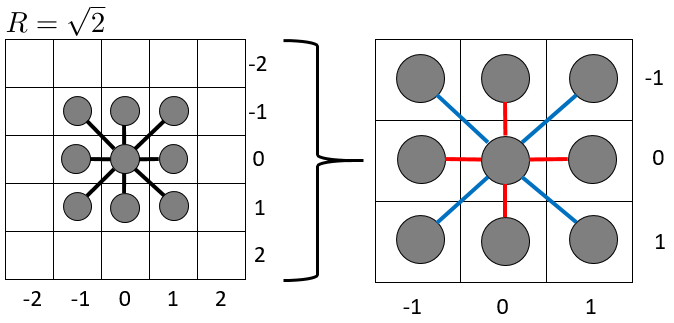
\includegraphics{img/fig-expansion-velocity.png}}
\end{center}\vspace*{-0.6cm}
\caption[Representaci\'on de las distintas velocidades de expansi\'on representadas en el modelo seg\'un la configuraci\'on de vecindad utilizada]{Representaci\'on de las distintas velocidades de expansi\'on representadas en el modelo seg\'un la configuraci\'on de vecindad utilizada. Las l\'ineas rojas en el diagrama derecho indican una mayor velocidad de expansi\'on que las l\'ineas azules. Esta noci\'on de velocidad se basa en la distancia entre estas c\'elulas.}
\label{fig-expansion-velocity}
\end{figure}

\begin{itemize}
\item [{XV.}] \textbf{Situaciones de competencia tumorales}: \emph{En las situaciones de competencia de varios tumores por expandirse a una misma posici\'on se asume que el valor de la probabilidad de transici\'on se corresponde con el tumor con mayor probabilidad de expansi\'on en ese momento. Si el tumor finalmente se expande hacia dicha posici\'on de forma satisfactoria, la nueva c\'elula cancer\'igena pertenece a dicho tumor.} \label{XV}

\item [{XVI.}] \textbf{Vectores de concentraci\'on de nutrientes}: \emph{Se asume que la concentraci\'on de nutrientes aumenta a medida que nos aproximamos a los tejidos de sost\'en y a la vasculatura del organismo. Este hecho se representa mediante uno o varios vectores en los \'organos del conjunto de c\'elulas del aut\'omata que indica las direcciones en que aumenta la concentraci\'on de los nutrientes.} \label{XVI}

\item [{XVII.}] \textbf{Sesgo direccional del crecimiento tumoral}: \emph{Se asume que la probabilidad de que aumente la poblaci\'on celular de un tumor se ve afectada por la concentraci\'on de los nutrientes. Este hecho constituye un sesgo en la direcci\'on del crecimiento del tumor, que se traduce en la tendencia a expandirse hacia la mayor concentraci\'on.} \label{XVII}

\item [XVIII.] \textbf{Velocidad de expansi\'on tumoral:} \emph{Se asume que la velocidad de expansi\'on tumoral depende de la distancia entre las c\'elulas tumorales y la c\'elula sana que intentan desplazar, que disminuye a medida que aumenta la distancia.} \label{XVIII}
\end{itemize}

La hipótesis XV se basa en la idea de que las proximidades de una neoplasia con un cierto nivel de desarrollo resulta en una menor concentración de nutrientes en comparación con un tejido sano, ya que la masa tumoral consume una cantidad significativa de los mismos. Por lo tanto, cualquier tumor con un desarrollo inferior, especialmente uno que tiene un bajo grado o nulo de vascularización, no tiende a expandirse hacia un tumor más grande que absorbe la mayoría de los nutrientes provenientes de la difusión. Esta suposición se fortalece con la hipótesis XVII y con la naturaleza oportunista y autoregulada del crecimiento tumoral. La hipótesis XVII permite explicar la expansión del tumor en las distintas capas de tejidos que conforman los órganos. Los tumores sólidos tienden a penetrar el estroma en busca de estos nutrientes, incluso si tienen una mayor densidad, lo que les permite crecer hacia el lumen del órgano aunque presente una densidad nula. Para representar estas nuevas hipótesis del modelo, es necesario reescribir la definición de la probabilidad de transición alternativa~(\ref{prop-newlocal-func}) como se muestra a continuación:

\begin{definition}
\label{prop-newlocal-func-2}
La funci\'on de transici\'on local definida en~\ref{prop-newlocal-func} se reescribe obteni\'endose una probabilidad de transici\'on alternativa que depende de nuevos argumentos:
\begin{equation}
s(v,n+1) = \mathcal{R}(S(v,n)) = e_i~~\textit{con probabilidad } \rho(\tau(v,n,N_{tum}) \rightarrow e_i), \label{eq-newlocal-func-2}
\end{equation}
donde $\tau(v,n,N_{tum})$ es una funci\'on que devuelve el conjunto de todos los tiempos transcurridos relativos al surgimiento de los tumores que intentan expandirse hacia $v$ en el instante de tiempo $n$; e.g. si los instantes de tiempo en que surgieron los tumores en cuesti\'on conforman el conjunto $\lbrace n_1', n_2', \ldots, n_m' \rbrace$ con $m$ la cantidad de tumores, el conjunto de tiempos transcurridos relativos es $n_r = \lbrace n-n_1',n-n_2', \ldots, n-n_m' \rbrace$.
\end{definition}

En el algoritmo~\ref{alg-n-r-2} se muestra la implementaci\'on de la nueva funci\'on $\tau(v,n,N_{tum})$ a modo de definici\'on donde se tiene en cuenta la hip\'otesis XV sobre las situaciones de competencia tumorales, $N^n(v)$ es la funci\'on de vecindad inmediata definida en~\ref{def-neighbourhoods}, la funci\'on $tumor(w)$ devuelve el identificador \'unico asociado al tumor al que pertenece $w$ y la funci\'on $s(w,n)$ es el estado de la c\'elula $w$ en el instante de tiempo $n$ definida en~\ref{def-cellstatus}. Se reescribe la regla del crecimiento tumoral~(\ref{eq-celldiv-2}) tomando en cuenta la nueva probabilidad de transici\'on alternativa~(\ref{eq-newlocal-func-2}) como:
\begin{equation}
s(v,n+1)=\mathcal{R}(S(v,n))=\left\lbrace
	\begin{array}{ll}
		\zeta_0(\tau(v,n,N_{tum}))& \textit{si } s(v,n)=0~\wedge~\mathcal{N}_3^n(S(v,n)) > 0 \\
		\zeta_1(\tau(v,n,N_{tum}))& \textit{si } s(v,n)=1~\wedge~\mathcal{N}_3^n(S(v,n)) > 0 \\
		\zeta_2(\tau(v,n,N_{tum}))& \textit{si } s(v,n)=2~\wedge~\mathcal{N}_3^n(S(v,n)) > 0 
	\end{array}
\right., \label{eq-celldiv-3}
\end{equation}
donde la distribuci\'on de probabilidad de las variables aleatorias $\zeta_i(\tau(v,n,N_{tum})) \in \lbrace i,3 \rbrace$ con $i \in \lbrace 0,1,2 \rbrace$ quedar\'ia como:
\begin{subequations}
\begin{equation}
P(\zeta_i(\tau(v,n,N_{tum}))=i) = 1 - \rho(\tau(v,n,N_{tum}) \rightarrow 3),
\end{equation}
\begin{equation}
P(\zeta_i(\tau(v,n,N_{tum}))=3) = \rho(\tau(v,n,N_{tum}) \rightarrow 3).
\end{equation}
\end{subequations}

\begin{algorithm}[t]
\caption{Definici\'on de la funci\'on $\tau(v,n,N_{tum})$.} \label{alg-n-r-2}
\KwData{$v, n, N_{tum}$}
\KwResult{$n_r$}
$n_r = \lbrace \rbrace$\;
\For{$w \in N^n(v)$}{
	\If{$s(w,n)=3$}{
		$n' = n - N_{tum}[tumor(w)]$\;
		$n_r = n_r \cup \lbrace n' \rbrace$\;}}
\Return $n_r$\;
\end{algorithm}

De acuerdo a la hip\'otesis XV sobre situaciones de competencia tumorales, la probabilidad de transici\'on~(\ref{eq-generaldivrule}) debe depender de las probabilidades de expansi\'on de cada uno de los tumores cuyos tiempos transcurridos relativos se encuentran en $\tau(v,n,N_{tum})$. Como se adopta la norma general que solo se expande el tumor con mayores posibilidades esta probabilidad de transici\'on puede ser escrita, tomando en cuenta la definici\'on~(\ref{prop-newlocal-func-2}), como:
\begin{equation}
\rho(\tau(v,n,N_{tum}) \rightarrow 3) = max\left[\rho(n_1 \rightarrow 3),\rho(n_2 \rightarrow 3),\ldots, \rho(n_m \rightarrow 3)\right], \label{eq-generaldivrule-2}
\end{equation}
donde $n_i \in \tau(v,n,N_{tum})$ con $i \in \lbrace 1,2,\ldots,m \rbrace$ y $m=|\tau(v,n,N_{tum})|$. La funci\'on $\rho(n_i \rightarrow 3)$ es la aplicaci\'on individual de la probabilidad de transici\'on a cada tumor contenido en el conjunto devuelto por la funci\'on $\tau(v,n,N_{tum})$. Se puede apreciar que el valor de la probabilidad de transici\'on global se corresponde con el m\'aximo de las probabilidades de expansi\'on de cada uno de los tumores que compiten por la posici\'on de la c\'elula $v$. La aplicaci\'on particular se escribe a partir de la probabilidad de transici\'on general del crecimiento tumoral~(\ref{eq-generaldivrule}):
\begin{equation}
\rho(n_i \rightarrow 3) = \left\lbrace
	\begin{array}{ll}
		\rho_a(n_i \Delta t)& \textit{si } n_i \leq n_a \\
		\rho_v((n_i - n_a) \Delta t)& \textit{si } n_i > n_a
	\end{array}
\right.. \label{eq-generaldivrule-3}
\end{equation}

Continuando con el proceso de incorporaci\'on de nuevas hip\'otesis a la probabilidad de transici\'on general del crecimiento tumoral, la hip\'otesis XVII sobre el sesgo direccional del crecimiento tumoral indica que la expansi\'on de un tumor tiende a producirse hacia una mayor concentraci\'on de nutrientes. Con el objetivo de simular la variaci\'on de dicha concentraci\'on en el tejido y tomando en cuenta la hip\'otesis XVI sobre los vectores de concentraci\'on de nutrientes se plantean las siguientes definiciones:

\begin{definition}
\label{def-regions}
Una regi\'on se define como:
\begin{equation}
R_i = \lbrace v~|~v \in V(G) : (x_{min} \leq v_x < x_{max})~\wedge~(y_{min} \leq v_y < y_{max}) \rbrace,
\end{equation}
donde $x_{min}$ y $y_{min}$ son los valores extremos inferiores de la regi\'on definida, mientras que $x_{max}$ y $y_{max}$ son los valores extremos superiores de la regi\'on definida. Las regiones definidas constituyen una partici\'on del conjunto de v\'ertices del grafo $V(G)$.
\end{definition}

\begin{definition}
\label{def-concentration}
Un vector de concentraci\'on expresa una direcci\'on hacia la cual aumenta el valor de la disponibilidad de nutrientes, tomando como regla general que el aumento ocurre en direcci\'on a los tejidos de sost\'en y a su vasculatura. Para simular condiciones heterog\'eneas en el interior de los \'organos cada uno de estos vectores est\'a asociado a una y solo una regi\'on dentro del mismo. El conjunto de vectores de concentraci\'on se denota como $B$, donde $B_i$ es el conjunto de vectores asociados al \'organo $i$ y $B_{ij}$ es el conjunto de vectores asociados al \'organo $i$ y a la regi\'on $R_j$ que pertenece a ese \'organo. 
\end{definition}

Por ejemplo en los diagramas izquierdo y centro de los cortes de tejidos mostrados en la figura~\ref{fig-structure} correspondientes con el aparato digestivo y las v\'ias a\'ereas inferiores del sistema respiratorio la variaci\'on de la concentraci\'on de nutrientes se puede representar mediante un vector que parte desde el tejido epitelial y apunta perpendicularmente hacia el estroma. En el caso del diagrama derecho de la figura~\ref{fig-structure} correspondiente con el h\'igado no hay necesidad de representar ning\'un vector ya que la vasculatura est\'a presente de manera uniforme en el \'organo haciendo de la concentraci\'on de nutrientes una magnitud homog\'enea. 

Generalmente se utiliza la similitud coseno para determinar el grado de similitud existente entre dos vectores mediante el valor del coseno del menor \'angulo comprendido entre ellos. En el presente trabajo se eval\'uan las similitudes coseno entre todos los vectores del conjunto $B$ que pertenecen a la regi\'on donde se localiza el tumor y el vector formado entre el centroide del tumor y la c\'elula $v$ hacia el que se est\'a expandiendo, tomando la mayor similitud como medida. Se interpreta esta medida como un coeficiente de las probabilidades de transici\'on de cada etapa del tumor $\rho_a(n \Delta t)$ y $\rho_v(n \Delta t)$, de manera el crecimiento se ve sesgado hacia la mayor concentraci\'on de nutrientes. A partir de lo expuesto anteriormente se plantean las siguientes definiciones:

\begin{definition}
\label{def-general-vector}
Sean dos c\'elulas $v$ y $w$ del conjunto $V(G)$. Un vector $\overrightarrow{\nu_{vw}}$ entre las c\'elulas $v$ y $w$ se define como:
\begin{equation}
\overrightarrow{\nu_{vw}} = \left(v_x - w_x, v_y - w_y \right). \label{eq-general-vector}
\end{equation}
\end{definition}

\begin{definition}
\label{def-sim}
Sean dos vectores $\overrightarrow{\nu_1}$ y $\overrightarrow{\nu_2}$, se define la similitud coseno $\beta(\overrightarrow{\nu_1},\overrightarrow{\nu_2})$ como el coseno del menor \'angulo, denotado como $\alpha$, comprendido entre ellos y se determina como:
\begin{equation}
\beta(\overrightarrow{\nu_1},\overrightarrow{\nu_2}) = \cos \alpha = \displaystyle\frac{\overrightarrow{\nu_1} \cdot \overrightarrow{\nu_2}}{|\overrightarrow{\nu_1}| \times |\overrightarrow{\nu_2}|}. \label{eq-sim}
\end{equation}
Como siempre toma el menor \'angulo comprendido entre los vectores, el mayor \'angulo comprendido posible es $\pi$ donde la similitud toma valor $-1$, que es el caso donde ambos vectores tienen direcciones opuestas. El menor \'angulo comprendido es $0$ donde la similitud toma valor $1$, correspondiente con el caso donde ambos vectores apuntan hacia la misma direcci\'on. La similitud toma valor $0$ cuando el \'angulo es $\pi /2$. Luego los valores posibles de la similitud coseno son:
\begin{equation}
\beta(\overrightarrow{\nu_1},\overrightarrow{\nu_2}) = \cos \alpha \in \left\lbrace
	\begin{array}{ll}
		\left[0,~1\right]& \textit{si } \alpha \in \left[0,\frac{\pi}{2} \right)\\
		\left[\textit{-}1,0\right]& \textit{si } \alpha \in \left[\frac{\pi}{2}, \pi \right]
	\end{array}
\right..
\end{equation}
\end{definition}

Como se observa, el valor de similitud varía entre $-1$ y $1$. La interpretación de los valores negativos puede ser problemática al usarlos como un coeficiente de probabilidad. Para penalizar el crecimiento tumoral opuesto a los vectores de concentración de nutrientes y favorecerlo cuando este crecimiento ocurre en la misma dirección, se utiliza una aplicación lineal que transforma el intervalo $[-1,1]$ de los valores de similitud en el intervalo $[0$.$5, 1$.$5]$. De esta manera, se penaliza la probabilidad de expansión al multiplicarse por $0$.$5$ si este crecimiento es contrario a la dirección indicada por los vectores de concentración de nutrientes, o se favorece al multiplicarse por $1$.$5$  si ocurre en la misma dirección que la indicada por los vectores de concentración de nutrientes. De esta forma, se mantiene el equilibrio del crecimiento tumoral. En caso de que una probabilidad supere el valor de $1$ al ser multiplicada por algún coeficiente definido en el presente modelo, su valor se establece en $1$. Es importante aclarar que si se considera el valor $0$ como penalización del crecimiento tumoral, se invalidaría la posibilidad de expansión contraria a la dirección indicada por los vectores de concentración de nutrientes. Esta nueva similitud alternativa se define a continuación:

\begin{definition}
\label{def-simprima}
Sean dos vectores $\overrightarrow{\nu_1}$ y $\overrightarrow{\nu_2}$, se define la similitud coseno alternativa $\beta_{alt}(\overrightarrow{\nu_1},\overrightarrow{\nu_2})$ como:
\begin{equation}
\beta_{alt}(\overrightarrow{\nu_1},\overrightarrow{\nu_2}) = \frac{1}{2} \beta(\overrightarrow{\nu_1},\overrightarrow{\nu_2}) + 1. \label{eq-simprima}
\end{equation}
La similitud coseno alternativa $\beta_{alt}(\overrightarrow{\nu_1},\overrightarrow{\nu_2}) \in [0$.$5, 1$.$5]$ cuando $\beta(\overrightarrow{\nu_1},\overrightarrow{\nu_2}) \in [-1, 1]$. 
\end{definition}

A partir de la expresi\'on~\ref{eq-simprima} se declara el coeficiente de la probabilidad de transici\'on $\beta_{tum}(v,l)$ como se muestra a continuaci\'on:

\begin{definition}
\label{def-beta}
La funci\'on $\beta_{tum}(v,l)$, que recibe una c\'elula $v$ y un tumor $l$, devuelve la m\'axima similitud coseno alternativa entre el vector $\overrightarrow{\nu_{vl}}$ y cada uno de los vectores de concentraci\'on del conjunto $B$ que pertenecen al mismo \'organo que el tumor $l$, es decir:
\begin{equation}
\beta_{tum}(v,l) = max\left[\beta_{alt}(\overrightarrow{b_{ij1}},\overrightarrow{\nu_{vl}}),\,\beta_{alt}(\overrightarrow{b_{ij2}}, \overrightarrow{\nu_{vl}})\,,\ldots,\,\beta_{alt}(\overrightarrow{b_{ijm}}, \overrightarrow{\nu_{vl}})\right], \label{eq-beta}
\end{equation}
donde $\overrightarrow{b_{ijk}} \in B_{ij}$ con $k \in \lbrace 1,2,\cdots,m \rbrace$ y $m=|B_{ij}|$ son los vectores de concentraci\'on asociados a la regi\'on $R_j$ del \'organo $i$ a la que pertenece la c\'elula $v$, o sea, $v \in R_j$, y $\overrightarrow{\nu_{vl}}$ es el vector formado por el c\'elula $v$ y el centroide del tumor $l$, donde el centroide constituye el punto de aplicaci\'on y $v$ el extremo del vector. 
\end{definition}

Las definiciones de un vector de expansi\'on y del centroide del tumor se presentan a continuaci\'on:

\begin{definition}
\label{def-centroid}
Sea $l=\lbrace w_1,w_2,\ldots,w_{m}\rbrace$ con $m=|l|$ un conjunto que contiene las c\'elulas pertenecientes a un tumor cualquiera representado en el aut\'omata. El centroide de dicho tumor se denota como $c_l$ y se define como el promedio de las componentes de las c\'elulas del conjunto, es decir:
\begin{equation}
c_l = \left(\frac{w_{1x} + w_{2x} + \ldots + w_{mx}}{m}, \frac{w_{1y} + w_{2y} + \ldots + w_{my}}{m} \right). \label{eq-centroid}
\end{equation}
\end{definition}

\begin{definition}
\label{def-exp-vector}
Sea el centroide $c_l$ de un tumor cualquiera $l$ y una c\'elula $v$ hacia el que se est\'a expandiendo dicho tumor. A partir de la expresi\'on~(\ref{eq-general-vector}) se define el vector de expansi\'on $\overrightarrow{\nu_{vl}}$ entre el centroide del tumor $c_l$ y la c\'elula $v$ como:
\begin{equation}
\overrightarrow{\nu_{vl}} = \left(v_x - c_{lx}, v_y - c_{ly} \right). \label{eq-exp-vector}
\end{equation}
\end{definition}

Seg\'un la hip\'otesis XVIII la velocidad de expansi\'on tumoral depende de la distancia a la que se encuentran las c\'elulas tumorales de las c\'elulas normales que intentan desplazar. La noci\'on consiste en tomar la mayor velocidad de entre todas las c\'elulas tumorales pertenecientes a un mismo tumor presentes en la vecindad de la c\'elula normal. Para este fin se definen las siguientes funciones:

\begin{definition}
\label{def-tumor-neighbourhood}
La funci\'on $N(v,l)$, que recibe una c\'elula normal $v$ y un tumor $l$, devuelve el conjunto de c\'elulas vecinas inmediatas de $v$ tales que pertenecen al tumor $l$ y que pertenezcan al mismo \'organo, es decir:
\begin{equation}
N(v,l) = \lbrace w~|~w \in \mathcal{N}^n(v)~\wedge~w \in l~\wedge~V_v(G) = V_w(G) \rbrace. \label{eq-tumor-neighbourhood}
\end{equation}
\end{definition}

\begin{definition}
\label{def-tumor-velocity}
La funci\'on $\gamma(v,w)$, que recibe una c\'elula normal $v$ y una tumoral $w$, devuelve la velocidad de expansi\'on tumoral en dependencia de la distancia euclideana~(Def. \ref{def-euclidean-distance}) existente entre ellas, es decir:
\begin{equation}
\gamma(v,w) = \left\lbrace
	\begin{array}{ll}
		0$.$5 & \textit{si } d_E(v,w) > 1 \\
		1$.$5 & \textit{si } d_E(v,w) = 1 
	\end{array}
\right.. \label{eq-tumor-velocity}
\end{equation}
\end{definition}

A partir de la expresi\'on~\ref{eq-tumor-velocity} se declara el coeficiente de la velocidad de expansi\'on tumoral $\gamma_{tum}(v,N(v,l))$ como se muestra a continuaci\'on:

\begin{definition}
\label{def-velocity-function}
La funci\'on $\gamma_{tum}(v,N(v,l))$, que recibe una c\'elula normal $v$ y las c\'elulas vecinas a esta $N(v,l)$ que pertenecen al tumor $l$, devuelve el m\'aximo valor de velocidad entre la c\'elula normal $v$ y cada una de las c\'elulas tumorales vecinas que pertenecen al conjunto $N(v,l)$, es decir:
\begin{equation}
\gamma_{tum}(v,N(v,l)) = max\left[\gamma(v,w_1), \gamma(v,w_2), \ldots \gamma(v,w_m) \right], \label{eq-velocity-function}
\end{equation}
donde $w_i \in N(v,l)$ con $i \in \lbrace 1,2,\cdots,m \rbrace$ y $m=|N(v,l)|$.
\end{definition}

Hasta el momento se han definido dos nuevos coeficientes de sesgo direccional del crecimiento tumoral $\beta_{tum}(v,l)$ y $\gamma_{tum}(v,N(v,l))$ que se desean incluir a la aplicaci\'on particular de la probabilidad de transici\'on general de la divisi\'on celular expuesta en~(\ref{eq-generaldivrule-3}). Con el objetivo de representar estas nuevas hip\'otesis del modelo es necesario reescribir la definici\'on de la probabilidad de transici\'on~(\ref{prop-newlocal-func-2}) como se muestra a continuaci\'on:

\begin{definition}
\label{prop-newlocal-func-2-1}
La funci\'on de transici\'on local definida en~\ref{prop-newlocal-func-2} se reescribe obteni\'endose una probabilidad de transici\'on alternativa que depende de nuevos argumentos:
\begin{equation}
s(v,n+1) = \mathcal{R}(S(v,n)) = e_i~~\textit{con probabilidad } \rho(v,\tau(v,n,N_{tum},L_{tum}) \rightarrow e_i), \label{eq-newlocal-func-2-1}
\end{equation}
donde $\tau(v,n,N_{tum},L_{tum})$ es una funci\'on que devuelve un conjunto compuesto por tuplas correspondientes con cada tumor que intenta expandirse hacia $v$ en el instante de tiempo $n$ que contienen el tiempo transcurrido relativo al surgimiento de dicho tumor y el conjunto de c\'elulas que lo conforman. El conjunto $L_{tum}$ contiene la informaci\'on correspondiente con los conjuntos de c\'elulas que conforman los tumores contenidos en la simulaci\'on.
\end{definition}

En el algoritmo~\ref{alg-L-c} se muestra la implementaci\'on de la funci\'on $\tau(v,n,N_{tum},L_{tum})$ a modo de definici\'on donde $N^n(v)$ es la funci\'on de vecindad inmediata definida en~\ref{def-neighbourhoods}, la funci\'on $tumor(w)$ devuelve el identificador \'unico asociado al tumor al que pertenece $w$ y la funci\'on $s(w,n)$ es el estado de la c\'elula $w$ en el instante de tiempo $n$ definida en~\ref{def-cellstatus}.

\begin{algorithm}[!ht]
\caption{Definici\'on de la funci\'on $\tau(v,n,N_{tum},L_{tum})$.} \label{alg-L-c}
\KwData{$v, n, N_{tum}, L_{tum}$}
\KwResult{$L$}
$L = \lbrace \rbrace$\;
\For{$w \in N^n(v)$}{
	\If{$s(w,n)=3$}{
		$l = L_{tum}[tumor(w)]$\;
		$n_r = n - N_{tum}[tumor(w)]$\;
		$L = L \cup \lbrace \langle n_r, l \rangle \rbrace$\;}}
\Return $L$\;
\end{algorithm}

Se reescribe la regla del crecimiento tumoral~(\ref{eq-celldiv-3}) tomando en cuenta la nueva probabilidad de transici\'on alternativa~(\ref{eq-newlocal-func-2-1}) como:
\begin{equation}
s(v,n+1)=\mathcal{R}(S(v,n))=\left\lbrace
	\begin{array}{ll}
		\zeta_0(v,\tau(v,n,N_{tum},L_{tum}))& \textit{si } s(v,n)=0~\wedge~\mathcal{N}_3^n(S(v,n)) > 0\\
		\zeta_1(v,\tau(v,n,N_{tum},L_{tum}))& \textit{si } s(v,n)=1~\wedge~\mathcal{N}_3^n(S(v,n)) > 0\\
		\zeta_2(v,\tau(v,n,N_{tum},L_{tum}))& \textit{si } s(v,n)=2~\wedge~\mathcal{N}_3^n(S(v,n)) > 0 \\
	\end{array}
\right., \label{eq-celldiv-3-1}
\end{equation}
donde la distribuci\'on de probabilidad de las variables aleatorias $\zeta_i(v,\tau(v,n,N_{tum},L_{tum}))$ $\in \lbrace i,3 \rbrace$ con $i \in \lbrace 0,1,2 \rbrace$ quedar\'ia como:
\begin{subequations}
\begin{align}
P(\zeta_i(v,\tau(v,n,N_{tum},L_{tum}))=i) &= 1 - \rho(v,\tau(v,n,N_{tum},L_{tum}) \rightarrow 3),\\
P(\zeta_i(v,\tau(v,n,N_{tum},L_{tum}))=3) &= \rho(v,\tau(v,n,N_{tum},L_{tum}) \rightarrow 3).
\end{align}
\end{subequations}

La probabilidad de transici\'on $\rho(v,\tau(v,n,N_{tum},L_{tum}) \rightarrow 3)$ se escribe de forma an\'aloga a la expresi\'on~(\ref{eq-generaldivrule-2}) de acuerdo a la hip\'otesis XV sobre situaciones de competencia tumorales y tomando en cuenta la definici\'on~(\ref{prop-newlocal-func-2-1}), como:
\begin{equation}
\rho(v,\tau(v,n,N_{tum},L_{tum}) \rightarrow 3) = max\left[\rho(v, n_1, l_1 \rightarrow 3),\rho(v, n_2, l_2 \rightarrow 3),\ldots, \rho(v, n_m, l_m \rightarrow 3)\right], \label{eq-generaldivrule-2-1}
\end{equation}
donde $n_i$ y $l_i$ son los valores de la tupla $\langle n_i, l_i \rangle \in \tau(v,n,N_{tum},L_{tum})$ con $i \in \lbrace 1,2,\ldots,m \rbrace$ y $m=|\tau(v,n,N_{tum},L_{tum})|$ correspondiente con el i-\'esimo tumor que se intenta expandir hacia $v$. La funci\'on $\rho(v, n_i, l_i \rightarrow 3)$ es la aplicaci\'on individual de la probabilidad de transici\'on a cada tumor contenido en el conjunto devuelto por la funci\'on $\tau(v,n,N_{tum},L_{tum})$. A partir de las expresiones~(\ref{eq-generaldivrule-2-1},~\ref{eq-beta},~\ref{eq-velocity-function}) se reescribe la aplicaci\'on particular de la probabilidad de transici\'on general de la divisi\'on celular como:
\begin{equation}
\rho(v,n_i,l_i \rightarrow 3) = \left\lbrace
	\begin{array}{ll}
		\gamma_{tum}(v,N(v,l_i))\,\beta_{tum}(v,l_i)\,\rho_a(n_i \Delta t)& \textit{si } n_i \leq n_a \\
		\gamma_{tum}(v,N(v,l_i))\,\beta_{tum}(v,l_i)\,\rho_v((n_i - n_a) \Delta t)& \textit{si } n_i > n_a
	\end{array}
\right.. \label{eq-generaldivrule-2-2}
\end{equation}

Finalmente, la probabilidad de transición general del crecimiento tumoral representa cómo las células normales son desplazadas por las células cancerosas de la masa tumoral, replicando diversas situaciones de competencia entre tumores, sesgos direccionales basados en la concentración de nutrientes y velocidades de expansión tumoral. Sin embargo, esta forma general aún no describe las mecánicas específicas de expansión tumoral hacia los distintos tipos de tejidos. Por lo tanto, es necesario especificar el cálculo de dicha probabilidad en función del tipo de célula normal desplazada.

\subsubsection{Probabilidades de transici\'on particulares}
Se ha definido hasta ahora una probabilidad de transición general del crecimiento tumoral, pero es evidente que la invasión de diferentes tipos de tejidos normales ocurre bajo condiciones específicas. Debido a los diversos tipos de células normales representadas en el autómata, se deben describir las condiciones que provocan la penetración de los tejidos conformados por dichas células. Como se mencionó al principio de esta sección, un tumor primario durante la etapa avascular es incapaz de invadir los tejidos de soporte pero su expansión puede ocurrir dentro del epitelio donde se originó y hacia el lumen, ambos procesos están influenciados por sesgos direccionales basados en los vectores de concentración de nutrientes. Es durante la etapa vascular cuando gana la capacidad de invadir el estroma debido a la angiogénesis. Un tumor secundario durante la etapa vascular tiene la capacidad de invadir el lumen, el epitelio y los tejidos de soporte del órgano, ya que constituye la evolución de una micrometástasis que ya poseía dichas capacidades. Las distribuciones de probabilidad de las variables aleatorias $\zeta_0(v,\tau(v,n,N_{tum},L_{tum}))$, $\zeta_1(v,\tau(v,n,N_{tum},L_{tum}))$ y $\zeta_2(v,\tau(v,n,N_{tum},L_{tum}))$ están planteadas en función de la probabilidad de transición general definida en~(\ref{eq-generaldivrule-2-2}), pero según las descripciones anteriores, es necesario escribir de forma particular cada probabilidad de transición según el tipo de célula desplazada. Luego, la distribución de probabilidad de estas variables aleatorias quedaría como:
\begin{subequations}
\begin{align}
P(\zeta_0(v,\tau(v,n,N_{tum},L_{tum}))=0) &= 1 - \rho_0(v,\tau(v,n,N_{tum},L_{tum}) \rightarrow 3),\\
P(\zeta_0(v,\tau(v,n,N_{tum},L_{tum}))=3) &= \rho_0(v,\tau(v,n,N_{tum},L_{tum}) \rightarrow 3),\\
P(\zeta_1(v,\tau(v,n,N_{tum},L_{tum}))=1) &= 1 - \rho_1(v,\tau(v,n,N_{tum},L_{tum}) \rightarrow 3),\\
P(\zeta_1(v,\tau(v,n,N_{tum},L_{tum}))=3) &= \rho_1(v,\tau(v,n,N_{tum},L_{tum}) \rightarrow 3),\\
P(\zeta_2(v,\tau(v,n,N_{tum},L_{tum}))=2) &= 1 - \rho_2(v,\tau(v,n,N_{tum},L_{tum}) \rightarrow 3),\\
P(\zeta_2(v,\tau(v,n,N_{tum},L_{tum}))=3) &= \rho_2(v,\tau(v,n,N_{tum},L_{tum}) \rightarrow 3),
\end{align}
\end{subequations}
donde se expone que la probabilidad de que una c\'elula normal sea desplazada de su posici\'on y cambie al estado $3$ depende de una probabilidad de transici\'on que constituye una particularizaci\'on de la probabilidad de transici\'on general~(\ref{eq-generaldivrule-2-2}). Se destaca que la probabilidad de transici\'on $\rho_2(v,\tau(v,n,N_{tum},L_{tum}) \rightarrow 3)$ es la encargada de describir la invasi\'on tumoral, y las probabilidades de transici\'on referentes al desplazamiento de las c\'elulas epiteliales y el lumen poseen la misma expresi\'on para su c\'alculo. Luego las probabilidades de transici\'on particulares $\rho_0(v,\tau(v,n,N_{tum},L_{tum}) \rightarrow 3)$ y $\rho_1(v,\tau(v,n,N_{tum},L_{tum}) \rightarrow 3)$ se reescriben como se muestra a continuaci\'on:
\begin{subequations}
\begin{equation}
\rho_0(v,\tau(v,n,N_{tum},L_{tum}) \rightarrow 3) = max\left[\rho_0(v,n_1,l_1 \rightarrow 3),\rho_0(v,n_2,l_2 \rightarrow 3),\ldots,\rho_0(v,n_m,l_m \rightarrow 3)\right], 
\end{equation}
\begin{equation}
\rho_1(v,\tau(v,n,N_{tum},L_{tum}) \rightarrow 3) = max\left[\rho_1(v,n_1,l_1 \rightarrow 3),\rho_1(v,n_2,l_2 \rightarrow 3),\ldots,\rho_1(v,n_m,l_m \rightarrow 3)\right], 
\end{equation}
\begin{equation}
\rho_0(v,n_i,l_i \rightarrow 3) =\left\lbrace
	\begin{array}{ll}
		\gamma_{tum}(v,N(v,l_i))\,\beta_{tum}(v,l_i)\,\rho_a(n_i \Delta t)& \textit{si } n_i \leq n_a \\
		\gamma_{tum}(v,N(v,l_i))\,\beta_{tum}(v,l_i)\,\rho_v((n_i - n_a) \Delta t)& \textit{si } n_i > n_a
	\end{array}
\right., 
\end{equation}
\begin{equation}
\rho_1(v,n_i,l_i \rightarrow 3) = \left\lbrace
	\begin{array}{ll}
		\gamma_{tum}(v,N(v,l_i))\,\beta_{tum}(v,l_i)\,\rho_a(n_i \Delta t)& \textit{si } n_i \leq n_a \\
		\gamma_{tum}(v,N(v,l_i))\,\beta_{tum}(v,l_i)\,\rho_v((n_i - n_a) \Delta t)& \textit{si } n_i > n_a
	\end{array}
\right., 
\end{equation}
\end{subequations}
donde $m=|\tau(v,n,N_{tum},L_{tum})|$. De las expresiones para el c\'alculo de $\rho_0(v,n_i,l_i \rightarrow 3)$ y $\rho_1(v,n_i,l_i$ $\rightarrow 3)$ se infiere que la expansi\'on de un tumor ocurre hacia estos dos tejidos durante las etapas avascular y vascular. La probabilidad de transici\'on particular $\rho_2(v,\tau(v,n,N_{tum},L_{tum}) \rightarrow 3)$ se reescribe como se muestra a continuaci\'on:
\begin{subequations}
\begin{equation}
\rho_2(v,\tau(v,n,N_{tum},L_{tum}) \rightarrow 3) = max\left[\rho_2(v,n_1,l_1 \rightarrow 3),\rho_2(v,n_2,l_2 \rightarrow 3),\ldots,\rho_2(v,n_m,l_m \rightarrow 3)\right], 
\end{equation}
\begin{equation}
\rho_2(v,n_i,l_i \rightarrow 3) = \left\lbrace
	\begin{array}{ll}
		0& \textit{si } n_i \leq n_a \\
		\gamma_{tum}(v,N(v,l_i))\,\beta_{tum}(v,l_i)\,\rho_v((n_i - n_a) \Delta t)& \textit{si } n_i > n_a
	\end{array}
\right., 
\end{equation}
\end{subequations}
donde $m=|\tau(v,n,N_{tum},L_{tum})|$. Se infiere de la expresi\'on para el c\'alculo de $\rho_2(v,n_i,l_i \rightarrow 3)$ que la expansi\'on de un tumor durante la etapa avascular no penetra el tejido de sost\'en, por tanto la probabilidad correspondiente se anula. Las expresiones anteriores pueden ser escritas de forma m\'as simple si utilizamos una funci\'on tipo Heaviside que devuelva el valor $1$ si el tumor $l$ est\'a en etapa avascular, o $0$ si est\'a en etapa vascular. Esta funci\'on se define como:

\begin{definition}
\label{def-heaviside}
La funci\'on $H(n)$, que recibe un instante de tiempo $n$, devuelve el valor $1$ si $n$ es menor o igual que $n_a$, o $0$ si es mayor estricto que $n_a$, es decir:
\begin{equation}
H(n) = \left\lbrace
	\begin{array}{ll}
		1& \textit{si } n \leq n_a \\ 
		0& \textit{si } n > n_a
	\end{array}
\right.. \label{eq-heaviside}
\end{equation}
\end{definition}

Finalmente las probabilidades de transici\'on $\rho_0(v,n_i,l_i \rightarrow 3)$, $\rho_1(v,n_i,l_i \rightarrow 3)$ y $\rho_2(v,n_i,l_i \rightarrow 3)$ utilizando la expresi\'on~\ref{eq-heaviside} quedan planteadas como se muestra a continuaci\'on:
\begin{subequations}
\begin{equation}
\rho_0(v,n_i,l_i \rightarrow 3) = \gamma_{tum}(v,N(v,l_i)) \beta_{tum}(v,l_i) \left[ H(n_i)\rho_a(n_i \Delta t) + (1-H(n_i))\rho_v((n_i - n_a) \Delta t) \right],
\end{equation}
\begin{equation}
\rho_1(v,n_i,l_i \rightarrow 3) = \gamma_{tum}(v,N(v,l_i)) \beta_{tum}(v,l_i) \left[ H(n_i)\rho_a(n_i \Delta t) + (1-H(n_i))\rho_v((n_i - n_a) \Delta t)\right],
\end{equation}
\begin{equation}
\rho_2(v,n_i,l_i \rightarrow 3) = (1-H(n_i)) \gamma_{tum}(v,N(v,l_i)) \beta_{tum}(v,l_i) \rho_v((n_i - n_a) \Delta t). 
\end{equation}
\end{subequations}

\subsection{Regla del surgimiento de c\'elulas migratorias}
\label{subsec-migrant}
A lo largo de esta seccion se presentan reglas que comprenden el comportamiento de las celulas cancerigenas migratorias, desde las condiciones de su surgimiento hata su desplazamiento a traves de la ECM del tejido de sosten. Es posible que una celula se mueva gracias a los cambios de la matriz de interaccion provocados por las proteinas involucradas en el control de la movilidad y la supresion de reguladores de la migracion. En (2.7) se expusieron los cambios que debe sufrir una celula cancerigena tumoral para que se transforme en una celula migratoria y consisten en la perdida de la capacidad de adhesion celular y alteraciones de la matriz de interaccion intercelular(Cambiar esta oracion).
%Las reglas que se presentan en esta sección abordan el comportamiento de las células cancerosas migratorias, desde su surgimiento hasta su desplazamiento a través de la ECM del tejido de soporte. En la sección~\ref{subsec-meta} se menciona que una célula cancerosa tumoral debe perder la capacidad de adhesión celular y experimentar cambios en la matriz de interacción intercelular para convertirse en una célula migratoria. El movimiento es posible debido a los cambios en la matriz de interacción que resultan en la expresión de proteínas implicadas en el control de la movilidad y la supresión de reguladores de la migración. En esta sección se definen las reglas relacionadas con el surgimiento de estas células para definir en secciones posteriores el proceso de migración y metástasis.

La metástasis es la última característica distintiva del cáncer en adquirirse, según la hipótesis II sobre las mutaciones de las células cancerosas, y solo ocurre cuando el tumor ya ha llevado a cabo la angiogénesis y su desarrollo está avanzado. En este modelo, se considera que una célula tumoral al dividirse tiene la posibilidad de generar un descendiente que presente las mutaciones relacionadas con la migración, y dependiendo de dónde surja, hay dos rutas principales que puede seguir para continuar la cascada metastásica. La primera ocurre cuando la célula progenitora surge en el borde del tumor, lo que causa su separación de la masa neoplásica y su avance a través de la ECM con el objetivo de encontrar un posible punto de penetración del sistema circulatorio. La segunda ocurre cuando la célula migratoria surge en el interior del tumor cerca de un capilar sanguíneo, lo que le permite penetrar directamente el sistema circulatorio sin necesidad de migración.Como la segunda situaci\'on parte directamente de la intravasaci\'on es conveniente concebirla en la secci\'on relacionada con la met\'astasis, una vez que se exponga la representaci\'on del transporte de estas c\'elulas a trav\'es del sistema circulatorio.

Para definir la regla que reproduce el surgimiento de células migratorias en la frontera del tumor, se siguen las ideas utilizadas en las reglas anteriores: se define el criterio de selección basado en el estado de la configuración local y la probabilidad de transición basada en la información del modelo continuo. Según esta primera situación, la descendencia de una célula cancerosa tiene la probabilidad de expresar un comportamiento migratorio si pertenece a la frontera de un tumor en un estado avanzado de su desarrollo. Sin embargo, como se explicó en la sección~\ref{subsec-states}, la migración ocurre exclusivamente en los tejidos representados como estroma, por lo que esta célula descendiente mutada solo desplaza a las células si su vecindad inmediata posee células normales correspondientes con el estroma. Por lo tanto, se sigue la idea planteada en la sección~\ref{subsec-celldiv} para definir el conjunto de reglas que describen el surgimiento de células tumorales: se definen las reglas que describen el surgimiento de las células migratorias a partir de la existencia de células tumorales en la vecindad de la ECM.
 
La variable aleatoria $\zeta_2(v,\tau(v,n,N_{tum},L_{tum}))$ presente en la regla del crecimiento tumoral expuesta en~(\ref{eq-celldiv-3-1}) que describe la aparici\'on de c\'elulas tumorales en el estroma puede tomar los valores $\lbrace 2,3 \rbrace$. Esta variable aleatoria se modifica para que pueda tomar uno de los valores siguientes $\lbrace 2,3,4 \rbrace$ de acuerdo a lo expresado anteriormente, lo que significa que una c\'elula perteneciente al estroma que est\'e en presencia de una c\'elula tumoral tiene la posibilidad de ser desplazada de su posici\'on por la descendencia de dicha c\'elula tumoral, y esta descendencia puede ser del tipo tumoral que permanece unida a la masa neopl\'asica o del tipo migratorio que posee las mutaciones necesarias para avanzar a trav\'es de la ECM. Luego la distribuci\'on de probabilidad de la variable aleatoria $\zeta_2(v,\tau(v,n,N_{tum},L_{tum}))$ quedar\'ia como:
\begin{subequations}
\begin{multline}
P(\zeta_2(v,\tau(v,n,N_{tum},L_{tum}))=2) = 1 - [\rho_2(v,\tau(v,n,N_{tum},L_{tum}) \rightarrow 3) + \\ \rho_2(v,\tau(v,n,N_{tum},L_{tum}) \rightarrow 4)],
\end{multline}
\begin{equation}
P(\zeta_2(v,\tau(v,n,N_{tum},L_{tum}))=3) = \rho_2(v,\tau(v,n,N_{tum},L_{tum}) \rightarrow 3),
\end{equation}
\begin{equation}
P(\zeta_2(v,\tau(v,n,N_{tum},L_{tum}))=4) = \rho_2(v,\tau(v,n,N_{tum},L_{tum}) \rightarrow 4).
\end{equation}
\end{subequations}

De las expresiones anteriores se infiere que una c\'elula perteneciente al estroma conserva su estado si no surge la descendencia cancer\'igena, ya sea tumoral o migratoria, y la probabilidad de surgimiento de dicha descendencia se determina mediante el c\'alculo de las funciones $\rho_2(v,\tau(v,n,N_{tum},L_{tum}) \rightarrow 3)$ y $\rho_2(v,\tau(v,n,N_{tum},L_{tum}) \rightarrow 4)$ respectivamente, donde la primera fue definida en la secci\'on~\ref{subsec-celldiv} mientras que la segunda ser\'a concebida a continuaci\'on. Con el objetivo de mantener la simplicidad y no tener que llevar a cabo alg\'un proceso de normalizaci\'on, nos aseguraremos que $\left[\rho_2(v,\tau(v,n,N_{tum},L_{tum}) \rightarrow 3) + \rho_2(v,\tau(v,n,N_{tum},L_{tum}) \rightarrow 4)\right] \in [0,1]$ para que la probabilidad $P(\zeta_2(v,\tau(v,n,N_{tum},L_{tum}))=2) \in [0,1]$. Se sigue la misma noci\'on planteada en la hip\'otesis XV sobre las situaciones de competencia tumorales, si una c\'elula perteneciente al estroma se encuentra en presencia de varios tumores la probabilidad de que surja una c\'elula migratoria se corresponde con el tumor que mayor probabilidad posee de producir esta descendencia, lo que provoca que la expresi\'on para el c\'alculo de $\rho_2(v,\tau(v,n,N_{tum},L_{tum}) \rightarrow 4)$ sea similar a la de $\rho_2(v,\tau(v,n,N_{tum},L_{tum}) \rightarrow 3)$, escrita como el m\'aximo de todas las probabilidades de expansi\'on correspondientes con los tumores en conflicto, es decir:
\begin{equation}
\rho_2(v,\tau(v,n,N_{tum},L_{tum}) \rightarrow 4) = max\left[\rho_2(n_1 \rightarrow 4),\,\rho_2(n_2 \rightarrow 4),\ldots,\,\rho_2(n_m \rightarrow 4)\right], \label{eq-generaldivrule-migration}
\end{equation}
donde $n_i$ es el valor del tiempo transcurrido relativo de la tupla $\langle n_i, l_i \rangle \in \tau(v,n,N_{tum},L_{tum})$ con $i \in \lbrace 1,2,\ldots,m \rbrace$ y $m=|\tau(v,n,N_{tum},L_{tum})|$. La funci\'on $\rho_2(n_i \rightarrow 4)$ es la aplicaci\'on individual de la probabilidad de transici\'on a cada tumor del conjunto que devuelve la funci\'on $\tau(v,n,N_{tum},L_{tum})$. La concepci\'on de las expresiones para el c\'alculo de las probabilidades individuales del surgimiento de c\'elulas migratorias de cada tumor se realiza de una forma m\'as emp\'irica y es un procedimiento que se repetir\'a en la concepci\'on de reglas futuras, pues aunque el objetivo del presente trabajo es reproducir todo el proceso de invasi\'on, migraci\'on y met\'astasis del c\'ancer de la forma m\'as realista y precisa posible haciendo uso de la informaci\'on proporcionada por el modelo de crecimiento log\'istico, estas expresiones constituyen un primer acercamiento a la representaci\'on matem\'atico-computacional de la cascada metast\'asica, fen\'omeno que a nuestro conocimiento no ha sido descrito de forma acertada por ning\'un trabajo previo.

La idea principal es hacer depender las probabilidades individuales del surgimiento de c\'elulas migratorias de la poblaci\'on del tumor en cuesti\'on seg\'un la ecuaci\'on de crecimiento log\'istico, de forma que a medida que aumente la poblaci\'on la probabilidad sea mayor. Se puede expresar como el cociente entre la poblaci\'on tumoral y la capacidad de carga del entorno seg\'un la etapa del desarrollo en que se encuentra el tumor. Dado que durante la etapa avascular esta probabilidad de transici\'on se anula se obtiene partir de la expresi\'on~(\ref{eq-verhulst-solution}) haciendo $t=n\Delta t$ la siguiente funci\'on para el c\'alculo de la poblaci\'on tumoral estimada durante la etapa vascular:
\begin{equation}
P_v(n \Delta t) = \frac{P_0^v K_v}{P_0^v + (K_v-P_0^v)e^{-r_v n \Delta t}}, \label{eq-verhulst-solution-2}
\end{equation}
Tomando en cuenta la hip\'otesis I sobre la progresi\'on idealizada del desarrollo tumoral del modelo que plantea la divisi\'on del desarrollo tumoral en dos etapas y la expresi\'on~(\ref{eq-verhulst-solution-2}) la funci\'on para el c\'alculo de la probabilidad de aparici\'on de c\'elulas migratorias queda como:
\begin{equation}
\rho_2(n_i \rightarrow 4) = \left\lbrace
	\begin{array}{cl}
		0& \textit{si } n_i \leq n_a \\
		\left( \displaystyle\frac{P_v((n_i - n_a) \Delta t)}{K_v + K_{mig}} \right)^{\displaystyle 1 / \eta_{mig}}& \textit{si } n_i>n_a
	\end{array}
\right., \label{eq-migrant-2}
\end{equation}
donde $\eta_{mig} \in (0,1]$ y $K_{mig} \in \mathbb{N}$ son par\'ametros que nos permiten ajustar el comportamiento de la regla. Mediante la variaci\'on de $\eta_{mig}$ se puede variar el instante de tiempo en el que comienza el surgimiento de c\'elulas migratorias y la variaci\'on de $K_{mig}$ permite establecer un l\'imite para la probabilidad de surgimiento de dichas c\'elulas migratorias. El aspecto clave reside en elegir valores para $\eta_{mig}$ y $K_{mig}$ que reproduzcan de forma realista el surgimiento de estas c\'elulas. En t\'erminos de la funci\'on tipo Heaviside definida en~\ref{def-heaviside} la probabilidad de transici\'on quedar\'ia como:
\begin{equation}
\rho_2(n_i \rightarrow 4) = (1-H(n_i)) \left( \displaystyle\frac{P_v((n_i - n_a) \Delta t)}{K_v + K_{mig}} \right)^{\displaystyle 1/\eta_{mig}}. \label{eq-migrant-3}
\end{equation}

Se debe aclarar que la implementaci\'on de esta regla puede traer situaciones de competencia con la regla del crecimiento tumoral. Por esta raz\'on en su implementaci\'on se da prioridad al crecimiento tumoral, es decir, si la regla del crecimiento tumoral no provoca la aparici\'on de una de c\'elula cancer\'igena de este tipo entonces se eval\'ua la posible aparici\'on de una c\'elula migratoria.

\subsection{Reglas de la migraci\'on}
\label{subsec-migration}
Una célula cancerosa migratoria que ha ingresado al estroma se desplaza a través del tejido a través de la degradación progresiva de la ECM hasta penetrar el sistema circulatorio en un posible punto de inserción. La representación de la migración de células cancerosas presenta un nuevo desafío técnico que se describe a continuación. En la secci\'on~\ref{subsec-function} se expuso que la funci\'on de transici\'on global~(\ref{eq-global-func-2}) no establece un orden de selecci\'on de las c\'elulas del aut\'omata para su actualizaci\'on. En el sentido cl\'asico los aut\'omatas celulares se actualizan de forma sincronizada, es decir, la aplicaci\'on de la funci\'on de transici\'on local es simult\'anea para todas las c\'elulas. No obstante, en muchas extensiones del modelo cl\'asico se recogen definiciones que permiten la implementaci\'on de la actualizaci\'on secuencial~\cite{book}, ya que permite la resoluci\'on de conflictos que aparecen frecuentemente en modelos sincronizados que representan el movimiento de alg\'un tipo de part\'icula~\cite{book}. Enti\'endase por part\'icula: mol\'ecula, c\'elula o unidad biol\'ogica individual claramente identificable. Por ejemplo: en un modelo sincronizado de movimiento, si dos part\'iculas se actualizan simult\'aneamente y eligen como destino una misma posici\'on, aparece una situaci\'on de competencia que no es posible resolver sin la aplicaci\'on de instrucciones especiales. Sin embargo, en un modelo secuencial una de las part\'iculas se elige primero para su actualizaci\'on, efect\'ua el movimiento y se modifican inmediatamente los estados. Por este motivo la posici\'on destino de la primera part\'icula aparece ocupada cuando la segunda part\'icula es elegida para ser actualizada, evit\'andose el conflicto. La actualizaci\'on secuencial puede traer consecuencias indeseadas si se utiliza un orden fijo como criterio de elecci\'on, ya que provoca la existencia de part\'iculas privilegiadas que siempre son seleccionadas con prioridad para su actualizaci\'on, lo que constituye una ventaja que les permite ocupar una posici\'on o obtener un recurso antes que otras part\'iculas de su mismo tipo. Por este motivo generalmente se define un orden aleatorio como criterio de elecci\'on en modelos secuenciales. En el presente modelo se adopta un enfoque h\'ibrido que utiliza las siguientes definiciones:

\begin{definition}
\label{modal}
Un conjunto de actualizaci\'on est\'a constituido por c\'elulas del aut\'omata que poseen el mismo m\'etodo de actualizaci\'on. Existen dos conjuntos modales: el conjunto de actualizaci\'on sincronizado $C^S(G)$ y el conjunto de actualizaci\'on secuencial $C^A(G)$. En el presente modelo se actualizan las c\'elulas de los conjuntos secuenciales y luego las c\'elulas de los conjuntos sincronizados.
\end{definition}

\begin{definition}
\label{sync-modal}
Un conjunto sincronizado $C^S(G)$ est\'a compuesto de c\'elulas del aut\'omata que se actualizan mediante la aplicaci\'on simult\'anea de la funci\'on de transici\'on local y los nuevos estados est\'an disponibles para las c\'elulas vecinas en el siguiente instante de tiempo. Dada la naturaleza simult\'anea de la aplicaci\'on de la funci\'on de transici\'on local no se requiere la definici\'on de un orden de actualizaci\'on para las c\'elulas de este conjunto.
\end{definition}

\begin{definition}
\label{async-modal}
Un conjunto secuencial $C^A(G)$ est\'a compuesto de c\'elulas del aut\'omata que al ser actualizadas los nuevos estados est\'an disponibles de manera inmediata, modificando las configuraciones locales de las c\'elulas vecinas en el mismo instante de tiempo. El orden de actualizaci\'on de las c\'elulas pertenecientes este conjunto se determina de manera aleatoria para evitar la existencia de c\'elulas privilegiadas.  
\end{definition}

Las definiciones anteriores juegan un papel fundamental en la implementaci\'on del aut\'omata ya que determinan el modo de actualizaci\'on de las c\'elulas. Una implementaci\'on b\'asica del procedimiento de actualizaci\'on h\'ibrido del presente modelo de aut\'omatas celulares se muestra en el algoritmo~\ref{alg-update}. Los conjuntos de actualizaci\'on se declaran en el momento que se define la configuraci\'on global inicial del conjunto de c\'elulas del aut\'omata y se van actualizando conforme avanza la ejecuci\'on. Las c\'elulas migratorias definen un conjunto de actualizaci\'on secuencial denotado como $C_{mig}^A(G)$, mientras que para las c\'elulas normales y tumorales del aut\'omata no es necesario definir un conjunto de actualizaci\'on espec\'ifico, simplemente son contenidas en el conjunto sincronizado modal $C^S(G)$\footnote{En las siguientes secciones a medida que se definan las reglas restantes de la funci\'on de transici\'on se especificar\'a a cu\'al conjunto de actualizaci\'on pertenece cada tipo de c\'elula.}. 

\begin{algorithm}[!ht]
\caption{Implementaci\'on b\'asica del procedimiento de actualizaci\'on del aut\'omata celular.}\label{alg-update}
\KwData{$G,\,C^A(G),\,C^S(G),\,S(n)$}
$updated=\lbrace \rbrace$\;
\While{$|C^A(G)|~\neq~|updated|$}{
	\Repeat{$v \notin updated$}{
		$v=Select$-$Random$-$Vertex(C^A(G))$\;}
	$Apply$-$Local$-$Transition$-$Function(v,\,S(n),\,G)$\;
	$updated = updated \cup v$\;}
\For{$v \in C^S(G)$}{
	$Apply$-$Local$-$Transition$-$Function(v,\,S(n),\,G)$\;}
\end{algorithm}

En el marco de nuestro modelo es de importancia reproducir la migraci\'on de c\'elulas cancer\'igenas con cierto grado de flexibilidad y con rangos de movimientos variables. En este sentido la idea de algunos investigadores~\cite{anderson,kansal3} ha sido definir vecindades de interacci\'on con un mayor radio de acci\'on o par\'ametros del modelo que indiquen la capacidad de movilidad de las c\'elulas. Con este objetivo se concibe un par\'ametro para el procedimiento de actualizaci\'on $\mu_{mig} \in \mathbb{N}$ que se corresponde con el rango m\'aximo del movimiento. Una c\'elula migratoria puede ser seleccionada para su actualizaci\'on un n\'umero de veces potencialmente igual al valor de $\mu_{mig}$. La incorporaci\'on de este par\'ametro y del conjunto de actualizaci\'on $C_{mig}^A(G)$ al algoritmo mostrado en~\ref{alg-update} posibilita la reproducci\'on de forma m\'as realista del movimiento de las c\'elulas cancer\'igenas. Los movimientos variables son posibles gracias a la configuraci\'on de vecindad utilizada mediante la posibilidad de que una c\'elula migratoria avance a una celda del aut\'omata m\'as distante. La implementaci\'on del procedimiento de actualizaci\'on, incorporando el par\'ametro definido y el conjunto de actualizaci\'on secuencial $C_{mig}^A(G)$, se muestra en los algoritmos~\ref{alg-update-2},~\ref{alg-update-2-1} y~\ref{alg-update-2-2} que constituyen las implementaciones del procedimiento de actualizaci\'on del aut\'omata celular y de los m\'etodos encargados de actualizar los conjuntos que contienen a las c\'elulas migratorias y a las c\'elulas normales y tumorales respectivamente\footnote{En las siguientes secciones a medida que se presenten nuevas modificaciones al procedimiento de actualizaci\'on del aut\'omata celular solo se expondr\'an los algoritmos y m\'etodos a los que corresponden dichas modificaciones.}. 

\begin{algorithm}[!ht]
\caption{Implementaci\'on del procedimiento de actualizaci\'on del aut\'omata celular incorporando el par\'ametro $\mu_{mig}$ y el conjunto de actualizaci\'on secuencial para las c\'elulas migratorias $C_{mig}^A(G)$.} \label{alg-update-2}
\KwData{$G,\,C_{mig}^A(G),\,C^S(G),\,S(n),\,\mu_{mig}$}
$Update$-$Migratory$-$Cells(G,\,C_{mig}^A(G),S(n),\,\mu_{mig})$\;
$Update$-$Synchronous$-$Cells(G,\,C^S(G),\,S(n))$\;
\end{algorithm}

\begin{algorithm}[!ht]
\caption{Implementaci\'on del m\'etodo $Update$-$Migratory$-$Cells(G,\,C_{mig}^A(G),\,S(n),$ $\mu_{mig})$ utilizado en el procedimiento de actualizaci\'on del aut\'omata celular y que se encarga de la actualizaci\'on del conjunto secuencial que contiene a las c\'elulas migratorias.} \label{alg-update-2-1}
\KwData{$G,\,C_{mig}^A(G),\,S(n),\,\mu_{mig}$}
$updated=\lbrace \rbrace$\;
$i=0$\;
\While{$i < \mu_{mig}$}{
	\While{$|C_{mig}^A(G)|~\neq~|updated|$}{
		\Repeat{$v \notin updated$}{
			$v=Select$-$Random$-$Vertex(C_{mig}^A(G))$\;}
		$Apply$-$Local$-$Transition$-$Function(v,\,S(n),\,G)$\;
		$updated = updated \cup v$\;}
	$updated=\lbrace \rbrace$\;	
	$i++$\;}
\end{algorithm}

\begin{algorithm}[!ht]
\caption{Implementaci\'on del m\'etodo $Update$-$Synchronous$-$Cells(G,\,C^S(G),\,S(n))$ utilizado en el procedimiento de actualizaci\'on del aut\'omata celular y que se encarga de la actualizaci\'on del conjunto sincronizado que contiene a las c\'elulas normales y tumorales.} \label{alg-update-2-2}
\KwData{$G,\,C^S(G),\,S(n)$}
\For{$v \in C^S(G)$}{
	$Apply$-$Local$-$Transition$-$Function(v,\,S(n),\,G)$\;}
\end{algorithm}

Una célula cancerosa migratoria utiliza tres elementos distintivos para desplazarse a través de la ECM hasta penetrar el sistema circulatorio. Estos elementos son esenciales para la migración ya que cada uno cumple una función específica. El primer elemento es una célula migratoria que avanza a través de la ECM gracias a un proceso de degradación que reduce la densidad o rigidez de la matriz extracelular, permitiendo su ocupación posterior. Este proceso ha sido estudiado por varios autores~\cite{kansal3,perumpanani,perumpanani2} y se ha demostrado que es el mecanismo que permite el movimiento de las células migratorias. Sin embargo, la dirección del movimiento se determina mediante la variación de la concentración de nutrientes en el entorno. Las células cancerosas tienden a moverse hacia la dirección de donde provienen los nutrientes de la difusión~\cite{kansal3,nutrients}. Finalmente, la capacidad de la célula cancerosa de sortear los distintos obstáculos que se presentan a lo largo del trayecto está dada por los distintos modos de migración que presentan. Su estrategia consiste en alternar entre estos modos de forma tal que cada uno sirve para enfrentarse a una situación concreta. Para adaptarse al medio pueden cambiar la estructura de la célula para atravesar espacios estrechos o expresar enlaces intercelulares en su superficie que se conectan a otras células cancerosas posibilitando la migración grupal. Con el objetivo de especificar claramente la representaci\'on de estos elementos en el presente modelo se plantea un nuevo conjunto de hip\'otesis:

\begin{itemize}
\item [{XIX.}] \textbf{Migraci\'on del c\'ancer}: \emph{En el presente modelo solo se representa la migraci\'on de c\'elulas individuales y no se hace distinci\'on entre sus distintos modos. En adici\'on se considera que durante su desplazamiento estas c\'elulas no se dividen.} \label{XIX}

\item [{XX.}] \textbf{Sesgo direccional de la migraci\'on}: \emph{El desplazamiento de las c\'elulas migratorias a trav\'es de la ECM del estroma est\'a condicionado por los vectores de concentraci\'on de nutrientes, que son determinantes en la selecci\'on de la direcci\'on de su movimiento. El proceso de degradaci\'on de la ECM no se representa en este modelo.} \label{XX}
\end{itemize}

El presente conjunto de reglas hace uso de una implementaci\'on conocida en la literatura~\cite{book} como intercambio de estados. En un modelo de actualizaci\'on secuencial que representa el movimiento de part\'iculas es com\'un que al efectuarse un desplazamiento los estados de la c\'elula origen y destino se intercambien mediante una actualizaci\'on simult\'anea de las dos c\'elulas involucradas. De esta forma la posici\'on origen quedar\'ia ocupada por la c\'elula destino del movimiento y la posici\'on destino quedar\'ia ocupada por la c\'elula que se desplaz\'o. Cabe se\~nalar que en nuestro modelo una c\'elula cancer\'igena solo se desplaza a trav\'es del estroma, lo que significa que siempre que se intercambien estados ser\'a entre una c\'elula migratoria y una c\'elula de este tejido.

Una c\'elula migratoria que haya sido elegida para su actualizaci\'on puede encontrarse en tres situaciones distintas: que en su vecindad inmediata no existan posiciones que puedan ser elegidas como destino de su movimiento lo que significa que est\'a inm\'ovil, que en su vecindad inmediata existan posibles destinos de su movimiento y, por \'ultimo, que posea una conexi\'on en su vecindad distante con una c\'elula que posee un estado perteneciente a los destinos v\'alidos de la met\'astasis. Esta \'ultima situaci\'on ser\'a abordada en la secci\'on~\ref{subsec-metastasis} y constituye el final de la migraci\'on ya que representa el arribo de una c\'elula cancer\'igena a un punto de inserci\'on, en el que penetra el sistema circulatorio y procede a llevar a cabo la met\'astasis. Comenzamos planteando una extensi\'on de la probabilidad de transici\'on expuesta en~\ref{def-local-func} de forma que reciba los argumentos requeridos en la definici\'on de la regla.

\begin{definition}
\label{prop-newlocal-func-4}
Sea una extensi\'on de la funci\'on de transici\'on local definida en~\ref{def-local-func} que incluye una probabilidad de transici\'on alternativa que depende de nuevos argumentos y se actualiza de forma secuencial:
\begin{equation}
s(v,n) = \mathcal{R}(S(v,n)) = e_i~~\textit{con probabilidad } \rho(\mu(v,n) \rightarrow e_i), \label{eq-newlocal-func-4}
\end{equation}
donde $\mu(v,n)$ es la cantidad de desplazamientos tentativos que ha realizado el individuo $v$ de la poblaci\'on en el instante de tiempo $n$. 
\end{definition}

La evaluaci\'on de la funci\'on $\mu(v,n)$ depende de la implementaci\'on del aut\'omata y se logra actualizando la cantidad de desplazamientos tentativos cada vez que la c\'elula $v$ es elegida para su actualizaci\'on. Un desplazamiento se considera tentativo se haya o no movido de su posici\'on la c\'elula en cuesti\'on. Es necesario definir nueva funci\'on $\mathcal{N}_{\mathcal{E'}}^d(S(v,n))$ como aparece a continuaci\'on:

\begin{definition}
\label{def-normal-distant-neighbours}
La funci\'on $\mathcal{N}_{\mathcal{E'}}^d(S(v,n))$, que recibe una configuraci\'on local $S(v,n)$ en el instante de tiempo $n$ centrada en una c\'elula $v$, devuelve la cantidad de c\'elulas presentes en la vecindad distante $\mathcal{N}^{d}(v)$ de dicha configuraci\'on local cuyos estados est\'en contenidos en el subconjunto de estados $\mathcal{E'} = \lbrace e_1, e_2, \ldots , e_{|\mathcal{E'}|}\rbrace \subseteq \mathcal{E}$.
\begin{equation}
\mathcal{N}_{\mathcal{E'}}^d(S(v,n)) = \sum_{\substack{{s(w_i,n) \in S(v,n)}\\{w_i \in \mathcal{N}^{d}(v)}}} \left[\delta(s(w_i,n),e_1) + \delta(s(w_i,n),e_2) + \ldots + \delta(s(w_i,n),e_{|\mathcal{E'}|}) \right]. \label{eq-normal-distant-neighbours}
\end{equation}
\end{definition}

Las reglas de las primeras dos situaciones se conciben teniendo en cuenta las hip\'otesis XIX y XX como se muestra a continuaci\'on:
\begin{equation}
s(v,n)=\mathcal{R}(S(v,n))=\left\lbrace
	\begin{array}{cl}
		\zeta_4(\mu(v,n)) & \textit{si } s(v,n)=4~\wedge~\mathcal{N}_{\mathcal{E}_{met}}^d(S(v,n))=0~\wedge\\
				          & \mathcal{N}_2^n(S(v,n))=0\\
		2& \textit{si } s(v,n)=4~\wedge~\mathcal{N}_{\mathcal{E}_{met}}^d(S(v,n))=0~\wedge\\
		 & \mathcal{N}_2^n(S(v,n))>0		
	\end{array}
\right., \label{eq-aparition}
\end{equation}
donde $\zeta_4(\mu(v,n)) \in \lbrace 2,4 \rbrace$ es una variable aleatoria que posee la siguiente distribuci\'on de probabilidad:
\begin{subequations}
\begin{equation}
P(\zeta_4(\mu(v,n))=2) = \rho_4(\mu(v,n) \rightarrow 2),
\end{equation}
\begin{equation}
P(\zeta_4(\mu(v,n))=4) = 1 - \rho_4(\mu(v,n) \rightarrow 2).
\end{equation}
\end{subequations}

Como se puede observar la primera regla se corresponde con la primera situaci\'on ya que la condici\'on $\mathcal{N}_{\mathcal{E}_{met}}^d(S(v,n))=0 \wedge \mathcal{N}_2^n(S(v,n))=0$ describe su incapacidad para desplazarse a trav\'es del estroma ni penetrar el sistema circulatorio. La condici\'on de la segunda regla $\mathcal{N}_{\mathcal{E}_{met}}^d(S(v,n))=0 \wedge \mathcal{N}_2^n(S(v,n))>0$ se corresponde con la situaci\'on donde existen posibles destinos que pueden ser seleccionados por la c\'elula cancer\'igena para llevar a cabo su desplazamiento. El conjunto ${\mathcal{E}_{met}}$ contiene los estados que constituyen destinos v\'alidos para la met\'astasis y se corresponden con c\'elulas pertenecientes al estroma, a un tumor o a una micromet\'astasis, es decir, ${\mathcal{E}_{met}} = \lbrace 2,3,5 \rbrace$. La discusi\'on sobre estos destinos v\'alidos se desarrollar\'a en la secci\'on~\ref{subsec-metastasis}. 

Si la c\'elula $v$ se encuentra inm\'ovil su estado final es el correspondiente con el valor que tome la variable aleatoria $\zeta_4(\mu(v,n))$. Si toma valor $2$ se asume que la existencia de la c\'elula migratoria $v$ termin\'o y la posici\'on dejada por ella es ocupada por el estroma. Si toma valor $4$ la c\'elula migratoria $v$ contin\'ua con su existencia pero permanece inm\'ovil. La capacidad de supervivencia de la c\'elula migratoria $v$ est\'a dada por la probabilidad de transici\'on $1-\rho_4(\mu(v,n) \rightarrow 2)$, de ah\'i que $\rho_4(\mu(v,n) \rightarrow 2)$ se corresponda con la probabilidad de muerte celular. Si la c\'elula $v$ tiene posibilidades de efectuar un desplazamiento, la posici\'on que ocupaba $v$ tomar\'a el valor $2$ del conjunto de estados correspondiente con el estroma como consecuencia del intercambio de estados. Cuando se aplica la regla del desplazamiento se actualiza simult\'aneamente el estado de la c\'elula destino $w$ como se muestra a continuaci\'on:
\begin{equation}
s(w,n) = \zeta_4(\mu(v,n)). \label{eq-interchange}
\end{equation}

De esta manera, la supervivencia de la c\'elula $v$ se prueba al ser seleccionada para su actualizaci\'on y estar en una situaci\'on donde no puede moverse, y al desplazarse a la posici\'on destino $w$. La concepci\'on de la probabilidad de transici\'on $\rho_4(\mu(v,n) \rightarrow 2)$ es similar a la de la probabilidad de transici\'on correspondiente con el surgimiento de c\'elulas migratorias, cuya expresi\'on se expone en~(\ref{eq-migrant-2}) y~(\ref{eq-migrant-3}). La supervivencia de una c\'elula migratoria depende de su interacci\'on con el sistema inmune, de la adquisici\'on de nutrientes durante el trayecto y de la obtenci\'on de enzimas que usualmente se generan en el medio donde se origin\'o la c\'elula, es decir, en el tumor~\cite{migration}. La idea es hacer depender la probabilidad de transici\'on de la cantidad de movimientos tentativos realizados en base a una cantidad promedio m\'axima expresada por un par\'ametro $\mu_{max} \in \mathbb{N}$, de forma que a medida que aumente la cantidad de movimientos tentativos, y por ende la distancia recorrida, la probabilidad de muerte celular sea mayor. Finalmente la expresi\'on queda como:
\begin{equation}
\rho_4(\mu(v,n) \rightarrow 2) = \left(\displaystyle\frac{\mu(v,n)}{\mu_{max}} \right)^{\displaystyle 1 / \eta_{mig}'}, \label{eq-rho-4}
\end{equation}
donde $\eta_{mig}' \in (0,1]$ es un par\'ametro que nos permite ajustar el comportamiento de la regla. Mediante la variaci\'on de $\eta_{mig}'$ se pueden representar condiciones favorables o adversas para la supervivencia de la c\'elula migratoria. Resta definir el proceso de selecci\'on de la posici\'on destino $w$. Dado que la migraci\'on de estas c\'elulas las lleva a alejarse del tumor que les dio origen siguiendo el gradiente de la concentraci\'on de nutrientes se plantea la funci\'on $\tau(v,L_{tum})$ que devuelve el conjunto de c\'elulas que conforman el tumor donde se origin\'o la c\'elula migratoria $v$. Esto se logra a trav\'es de la funci\'on $tumor(v)$, mostrada en los algoritmos~\ref{alg-n-r}, \ref{alg-n-r-2} y \ref{alg-L-c}, que en caso de que $v$ sea una c\'elula migratoria devuelve el identificador \'unico de dicho tumor. Luego se define la siguiente funci\'on:

\begin{definition}
\label{def-type-neighbours}
La funci\'on $D_{mig}(v,n)$, que recibe una c\'elula migratoria $v$ y un instante de tiempo $n$, devuelve el conjunto de c\'elulas vecinas inmediatas de $v$ tales que su estado en el instante de tiempo $n$ sea igual a $2$ y que pertenezcan al mismo \'organo, es decir:
\begin{equation}
D_{mig}(v,n) = \lbrace w~|~w \in \mathcal{N}^n(v)~\wedge~s(w,n)=2~\wedge~V_v(G) = V_w(G)~\wedge~d_E(c_l,w) > d_E(c_l,v) \rbrace, \label{eq-type-neighbours}
\end{equation}
donde $\tau(v,L_{tum}) = l$ y la condici\'on $d_E(c_l,w) > d_E(c_l,v)$ asegura que los posibles movimientos de la c\'elula $v$ siempre la alejen del tumor donde se origin\'o.
\end{definition}

La selecci\'on de la posici\'on destino comienza evaluando la funci\'on~(\ref{eq-type-neighbours}) en la c\'elula $v$ en el instante de tiempo actual, obteniendo un conjunto de posibles destinos de la forma $D_{mig}(v,n) = \lbrace w_1, w_2, \ldots, w_m \rbrace$ donde $m=|D_{mig}(v,n)|$. Seg\'un la hip\'otesis XX sobre el sesgo direccional de la migraci\'on, la direcci\'on del movimiento se determina en base a los vectores de concentraci\'on de nutrientes del conjunto $B$. Entre la c\'elula migratoria $v$ y cada una de las c\'elulas destino del conjunto $D_{mig}(v,n)$ se forman vectores de desplazamiento, y para cada uno de estos vectores se estima la probabilidad de que la c\'elula $v$ lo seleccione como la direcci\'on final del movimiento. Esta probabilidad se determina como la m\'axima similitud coseno alternativa entre cada vector de direcci\'on y los vectores de concentraci\'on de nutrientes. Estamos en condiciones de definir la funci\'on para la selecci\'on de la posici\'on destino:

\begin{definition}
\label{def-dest-selection}
La funci\'on $d_{mig}(v,n)$, que recibe una c\'elula $v$ y un instante de tiempo $n$, devuelve una c\'elula $w$ que pertenece al conjunto $D_{mig}(v,n)$ y constituye el destino elegido para la migraci\'on de la c\'elula $v$. El procedimiento queda de la siguiente forma:
\begin{equation}
d_{mig}(v,n) = \left\lbrace
	\begin{array}{ll}
		w_1 & \textit{con probabilidad } \frac{1}{m} \beta_{mig}(v,w_1)\\
		w_2 & \textit{con probabilidad } \frac{1}{m} \beta_{mig}(v,w_2)\\
		\vdots & \ldots\\
		w_m & \textit{con probabilidad } \frac{1}{m} \beta_{mig}(v,w_m)
	\end{array}
\right., \label{eq-dest-selection}
\end{equation}
donde $D_{mig}(v,n)= \lbrace w_1,w_2,\ldots,w_m \rbrace$ con $m = |D_{mig}(v,n)|$. Este sesgo se determina como el m\'aximo valor de las similitudes coseno alternativa entre el vector de desplazamiento formado por $v$ y $w$ y cada uno de los vectores de concentraci\'on de nutrientes $B_{ij} = \lbrace \overrightarrow{b_{ij1}}, \overrightarrow{b_{ij2}}, \ldots, \overrightarrow{b_{ijm'}} \rbrace$ donde $m'=|B_{ij}|$ asociados a la regi\'on $R_j^c$ a la que pertenece $w$, es decir:
\begin{equation}
\beta_{mig}(v,w) = max\left[\beta_{alt}(\overrightarrow{b_{ij1}},\overrightarrow{\nu_{vw}}), \beta_{alt}(\overrightarrow{b_{ij2}},\overrightarrow{\nu_{vw}}), \ldots, \beta_{alt}(\overrightarrow{b_{ijm'}},\overrightarrow{\nu_{vw}})\right], \label{eq-dest-selection-2}
\end{equation}
donde $\overrightarrow{\nu_{vw}}$ es el vector de desplazamiento que se define de forma an\'aloga al vector de expansi\'on expuesto en~\ref{def-exp-vector}:
\begin{equation}
\overrightarrow{\nu_{vw}} = \left(v_x - w_{x}, v_y - w_{y}\right). \label{eq-dest-selection-vector}
\end{equation}
\end{definition}

La funci\'on $\beta_{mig}(v,w)$, que recibe la c\'elula migratoria $v$ y una c\'elula $w \in D_{mig}(v,n)$ se utiliza como un coeficiente de la probabilidad de que la c\'elula $w$ sea seleccionada como destino del movimiento y constituye un sesgo direccional. Como se puede apreciar en~\ref{def-dest-selection} la elecci\'on del destino del movimiento se lleva a cabo de forma aleatoria entre los posibles destinos que se beneficien de los vectores de concentraci\'on de nutrientes y aumenten la distancia entre la c\'elula $v$ y el tumor donde se origin\'o la migraci\'on. Pero la utilizaci\'on de la funci\'on~(\ref{eq-dest-selection}) en esta forma tiene un problema. El criterio de selecci\'on de la regla para la migraci\'on de una c\'elula que tiene posibles movimientos enumera todos los destinos posibles, incluidas las posiciones que la hacen acercarse al tumor. Luego puede existir la situaci\'on donde una c\'elula migratoria se elige para su actualizaci\'on, se verifique que posee movimientos posibles pero todos los movimientos posibles la acerquen al tumor, por lo que la funci\'on $D_{mig}(v,n)$ no devuelva posici\'on alguna. Este caso extremo se puede resolver modificando la funci\'on~(\ref{eq-dest-selection}) como se muestra a continuaci\'on:

\begin{definition}
\label{def-dest-selection-2}
La funci\'on $d_{mig}(v,n)$ se modifica de la siguiente forma para que tome en cuenta el caso extremo donde el conjunto devuelto por $D_{mig}(v,n)$ sea vac\'io:
\begin{equation}
d_{mig}(v,n) = \left\lbrace
	\begin{array}{ll}
		v & \textit{si } |D_{mig}(v,n)|=0\\
		d_{mig}'(v,n)& \textit{si } |D_{mig}(v,n)|\neq 0		
	\end{array}
\right.. \label{eq-dest-selection-3}
\end{equation}
Como se puede apreciar la soluci\'on es devolver la misma c\'elula $v$ como destino, hecho que no altera a la definici\'on de la regla y eval\'ua satisfactoriamente la supervivencia de $v$, tal como ocurrir\'ia en el caso donde la c\'elula $v$ est\'a inm\'ovil. Al seleccionarse la propia posici\'on original de $v$, su estado es actualizado mediante la expresi\'on~(\ref{eq-interchange}). La funci\'on $d_{mig}'(v,n)$ se corresponde con la definici\'on anterior mostrada en~\ref{def-dest-selection}, es decir:
\begin{equation}
d_{mig}'(v,n) = \left\lbrace
	\begin{array}{ll}
		w_1 & \textit{con probabilidad } \frac{1}{m} \beta_{mig}(v,w_1)\\
		w_2 & \textit{con probabilidad } \frac{1}{m} \beta_{mig}(v,w_2)\\
		\vdots & \ldots\\
		w_m & \textit{con probabilidad } \frac{1}{m} \beta_{mig}(v,w_m)
	\end{array}\
\right., \label{eq-dest-selection-4}
\end{equation}
donde $D_{mig}(v,n)= \lbrace w_1,w_2,\ldots,w_m \rbrace$ con $m = |D_{mig}(v,n)|$.
\end{definition}

En la secci\'on~\ref{subsec-metastasis} siguiente se define la regla que da culminaci\'on al proceso migratorio del c\'ancer: la met\'astasis, que describe la inserci\'on de la c\'elula migratoria en el sistema circulatorio y su arribo a la nueva localizaci\'on.

\subsection{Regla de la met\'astasis}
\label{subsec-metastasis}
Seg\'un las reglas definidas en las secciones~\ref{subsec-migrant} y~\ref{subsec-migration} existen dos posibles rutas para que aparezca una c\'elula cancer\'igena migratoria y lleve a cabo la met\'astasis de forma satisfactoria. El punto de partida de ambas rutas est\'a contenido en el criterio de selecci\'on de la regla del surgimiento de c\'elulas migratorias. La primera ruta comprende la migraci\'on de una c\'elula cancer\'igena desde la frontera del tumor al que pertenece hasta penetrar el sistema circulatorio en un posible punto de inserci\'on. En esta ruta la condici\'on inicial que reproduce el surgimiento de la c\'elula migratoria est\'a dada por $\mathcal{N}_{\mathcal{E}_{met}}^d(S(v,n))=0 \wedge \mathcal{N}_2^n(S(v,n))>0$ que expresa la inexistencia de una conexi\'on distante viable para una posible met\'astasis y que pertenece a la frontera de un tumor que penetr\'o el tejido correspondiente con el estroma. A medida que esta c\'elula avanza a trav\'es del estroma se verifica en la regla de la migraci\'on si esta c\'elula entra en contacto con una conexi\'on distante viable. Si lo hace pasa a penetrar el sistema circulatorio, sino contin\'ua su avance. La segunda ruta describe la situaci\'on de una c\'elula tumoral que est\'e desde un inicio en contacto con una conexi\'on distante viable. En este caso es posible que la progenie de dicha c\'elula cancer\'igena muestre las mutaciones relacionadas con la migraci\'on y proceda a su inserci\'on en el sistema circulatorio. Estas rutas se representan en la figura~\ref{fig-metastasis-vias}.

\begin{figure}[!ht]
\begin{center}
\scalebox{0.5}{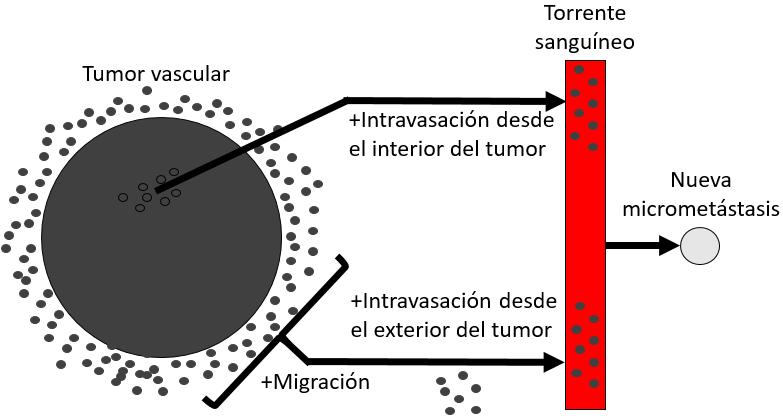
\includegraphics{img/fig-metastasis-vias.png}}
\end{center}\vspace*{-0.6cm}
\caption[Descripci\'on de las distintas rutas de la met\'astasis del c\'ancer]{Descripci\'on de las distintas rutas de la met\'astasis del c\'ancer. Las c\'elulas cancer\'igenas que presentan mutaciones que les permiten migrar a trav\'es de la ECM pueden llevar a cabo la met\'astasis despu\'es de concluir el desplazamiento desde la frontera del tumor hasta un capilar sangu\'ineo presente en los tejidos de sost\'en o desde el interior del propio tumor a trav\'es de los capilares sangu\'ineos que crecen en su interior producto de la angiog\'enesis.}
\label{fig-metastasis-vias}
\end{figure}

Una célula cancerosa migratoria que ha penetrado en el sistema circulatorio se enfrenta a varios peligros que pueden resultar en su muerte, incluyendo las defensas del sistema inmunológico que pueden reconocer y destruir estas células, así como el estrés mecánico al que son sometidas al ser transportadas a través de capilares sanguíneos de menor diámetro que la propia célula. Eventualmente, se adhiere a un posible punto de extravasación, degradando la pared del vaso sanguíneo y abandonando el sistema circulatorio. Hasta ahora no existe un método para determinar de manera realista la probabilidad de supervivencia de la célula cancerosa durante su transporte por el sistema circulatorio ni para predecir la ubicación donde dicha célula abandonará el torrente sanguíneo, ya que es un fenómeno sujeto a muchos procesos aleatorios. Como se expres\'o en la secci\'on~\ref{subsec-meta} la teor\'ia de la semilla y el sustrato es ampliamente aceptada porque permite explicar la tendencia del c\'ancer de colonizar \'organos espec\'ificos. Bas\'andonos en esta teor\'ia se a\~naden un conjunto de hip\'otesis al modelo que permiten representar la met\'astasis del c\'ancer:

\begin{itemize}
\item [XXI.] \textbf{Conexiones distantes del grafo}: \emph{Cada \'organo representado est\'a vinculado con el otro a trav\'es de las conexiones distantes existentes en el grafo subyacente. Se asume que una c\'elula que penetre el sistema circulatorio en un punto dado lo abandonar\'a en una posici\'on predeterminada, correspondientes con los destinos de las conexiones mencionadas.} \label{XXI}
\end{itemize}

La hip\'otesis XXI se apoya en la consideraci\'on que expresa que un tejido vivo puede ser representado mediante una red de mundo peque\~no, planteada en la secci\'on~\ref{subsec-hipo}. El presente modelo reproduce las localizaciones correspondientes con el \'organo donde se origin\'o el tumor y un \'organo que es colonizado de forma preferencial por el tipo de c\'ancer en cuesti\'on, pero es necesario a\~nadir a estas localizaciones una forma que representar las c\'elulas migratorias que permanecen en el interior del sistema circulatorio. La representaci\'on de este transporte a trav\'es del sistema circulatorio debe permitir reproducir la duraci\'on del trayecto y evaluar su supervivencia. 

Supongamos que tenemos una célula que tiene una conexión distante, y debido a esta conexión, tiene la posibilidad de convertirse en un destino potencial para la metástasis. Para representar la migración, se establece un conjunto que contiene la información de todas las células migratorias que están viajando a través del sistema circulatorio hacia sus destinos. Cuando una célula migratoria llega a una posición que tiene una conexión distante con una célula del estroma que aún no ha sido colonizada, la célula migratoria abandona su posición y se une al conjunto definido anteriormente. Una vez en este conjunto, en cada momento se verifica su supervivencia hasta que abandona el sistema circulatorio para colonizar finalmente la posición destino. Este proceso describe a grandes rasgos la idea detrás de la metástasis, pero el destino no tiene que ser necesariamente una célula del estroma para que la célula migratoria lo considere un destino viable para la metástasis. El destino puede ser una célula del estroma, una célula de un tumor o una célula de una micrometástasis. Cada uno de estos destinos se corresponde con las distintas situaciones expuestas en la secci\'on~\ref{subsec-meta} que pueden ocurrir cuando una célula migratoria abandona el sistema circulatorio en una ubicación, de ah\'i que el conjunto que contiene los posibles destinos de la met\'astasis tenga la forma ${\mathcal{E}_{met}}=\lbrace 2,3,5 \rbrace$. Si la c\'elula destino es una c\'elula de un tumor o es alguna micromet\'astasis se infiere que si la c\'elula migratoria sobrevive al transporte y extravasa satisfactoriamente, esta contribuye con la poblaci\'on de dichos tumores. Si la c\'elula destino es una c\'elula del estroma, entonces se crear\'a un nuevo foco cancer\'igeno. No obstante, est\'a fuera del alcance del presente modelo representar estas contribuciones a las poblaciones tumorales. Luego, las c\'elulas migratorias siempre penetran el sistema circulatorio si entran en contacto con una conexi\'on distante, pero solo se almacenan y eval\'uan las que tienen como destino una c\'elula del estroma o una micromet\'astasis, ya que estos tumores pueden ser eliminados por el sistema inmunitario y se debe poder representar la recreaci\'on de estos focos cancerosos. Luego se plantea la siguiente hip\'otesis: 

\begin{itemize}
\item [XXII.] \textbf{Destinos viables de la met\'astasis}: \emph{Se representan solamente las migraciones de c\'elulas cancer\'igenas hacia localizaciones que est\'an sin colonizar o que se corresponden con una micromet\'astasis. Si las localizaciones destino se corresponde con un tumor la c\'elula migratoria abandona su posici\'on y penetra el sistema circulatorio pero no se eval\'ua su transporte ni el arribo a la nueva localizaci\'on.} \label{XXII}
\end{itemize}

Como en el conjunto que representa el sistema circulatorio existen c\'elulas migratorias que poseen una misma posici\'on destino es necesario que sean actualizadas de forma secuencial para manejar las distintas situaciones de competencia, y al igual que sucede con la migraci\'on el orden de actualizaci\'on es aleatorio. La implementaci\'on del los conjunto que representa el sistema circulatorio se logra mediante un conjunto de actualizaci\'on secuencial $C_{sc}^A(G)$ en el que se almacena la informaci\'on referente a las c\'elula migratorias y su destino. Se define un nuevo par\'ametro $\xi_{sc} \in [0,1]$ que es la probabilidad de supervivencia de la c\'elula migratoria en el sistema circulatorio. La incorporaci\'on del conjunto de actualizaci\'on $C_{sc}^A(G)$ y de este par\'ametro al procedimiento de actualizaci\'on se muestra en el algoritmo~\ref{alg-update-3}. El m\'etodo encargado de actualizar las c\'elulas contenidas en el torrente sangu\'ineo se muestra en el algoritmo~\ref{alg-update-3-1}. Como se puede observar en el algoritmo~\ref{alg-update-3}, el transporte en el interior del sistema circulatorio se eval\'ua inicialmente, de forma tal que las c\'elulas que lo penetren como consecuencia de la actualizaci\'on de las c\'elulas migratorias no sean evaluadas hasta el instante de tiempo siguiente.

\begin{algorithm}[!ht]
\caption{Implementaci\'on del procedimiento de actualizaci\'on del aut\'omata celular incorporando el par\'ametro $\xi_{sc}$ y el conjunto de actualizaci\'on secuencial para las c\'elulas migratorias en el interior del sistema circulatorio $C_{sc}^A(G)$.} \label{alg-update-3}
\KwData{$G,\,C_{mig}^A(G),\,C_{sc}^A(G),\,C^S(G),\,S(n),\,\mu_{mig},\,\xi_{sc}$}
$Update$-$Migratory$-$Cells$-$In$-$Bloodstream(C_{sc}^A(G),\,\xi_{sc})$\;
$Update$-$Migratory$-$Cells(G,\,C_{mig}^A(G),\,S(n),\,\mu_{mig})$\;
$Update$-$Synchronous$-$Cells(G,\,C^S(G),S(n))$\;
\end{algorithm}

\begin{algorithm}[!ht]
\caption{Implementaci\'on del m\'etodo $Update$-$Migratory$-$Cells$-$In$-$Bloodstream$ $(C_{sc}^A(G),\xi_{sc})$ utilizado en el procedimiento de actualizaci\'on del aut\'omata celular y que se encarga de la actualizaci\'on del conjunto secuencial que contiene a las c\'elulas migratorias contenidas en el torrente sangu\'ineo.} \label{alg-update-3-1}
\KwData{$C_{sc}^A(G),\,\xi_{sc}$}
\While{$|C_{sc}^A(G)|~\neq~0$}{
	$v=Select$-$Random$-$Vertex(C_{sc}^A(G))$\;
	$w=Get$-$Target$-$Vertex(v,\,C_{sc}^A(G))$\;
	\If{$Random(0,1) \leq \xi_{sc} \wedge s(w,n) = 2$}{		
		$Create$-$New$-$Metastasis(w)$\;}
	$Remove$-$Cell$-$From$-$Bloodstream(v,\,C_{sc}^A(G))$\;}
\end{algorithm}

El algoritmo~\ref{alg-update-3-1} describe el proceso de transporte y extravasaci\'on de las c\'elulas migratorias, luego resta definir el proceso de inserci\'on en el sistema circulatorio. Como se expres\'o anteriormente existen dos posibles situaciones en las que una c\'elula migratoria penetra el torrente sangu\'ineo. Para representar la primera situaci\'on en que la c\'elula migratoria parte desde la frontera del tumor y arriba a un posible punto de intravasaci\'on, se plantea una regla del aut\'omata celular, mientras que para la segunda situaci\'on en la que una c\'elula tumoral provoca el surgimiento de una c\'elula migratoria que penetra directamente el torrente sangu\'ineo, se agregan las instrucciones necesarias al algoritmo~\ref{alg-update-3} en las l\'ineas correspondientes con la actualizaci\'on del conjunto sincronizado $C^S(G)$ para representar dicha situaci\'on. Estas modificaciones consisten en verificar la existencia de una c\'elula tumoral en presencia de una conexi\'on distante, que en caso afirmativo se a\~nade una c\'elula migratoria a la representaci\'on del torrente sangu\'ineo con el destino correspondiente. Una observaci\'on importante es que una misma c\'elula puede poseer m\'as de una conexi\'on distante producto de la aleatoriedad del proceso de reconexi\'on del modelo Watts-Strogatz. Por tanto se sigue el mismo esquema de la regla de la migraci\'on: actualizar el estado de la c\'elula mediante la aplicaci\'on de la regla de la met\'astasis y elegir de forma aleatoria el destino. 

Comenzamos definiendo la regla para la primera situaci\'on descrita anteriormente. Como se expuso en la secci\'on~\ref{subsec-migration} el final de la migraci\'on est\'a dada por la existencia de una conexi\'on distante viable para la met\'astasis en la posici\'on actual de la c\'elula migratoria. Esta condici\'on constituye el criterio de selecci\'on de la regla para la met\'astasis como se muestra a continuaci\'on:
\begin{equation}
s(v,n)=\mathcal{R}(S(v,n))= 2~~\textit{si } s(v,n)=4~\wedge~\mathcal{N}_{\mathcal{E}_{met}}^d(S(v,n))>0. \label{eq-intravasation}
\end{equation}

Se puede apreciar en la expresi\'on~(\ref{eq-intravasation}) que la regla posee un car\'acter determinista, ya que su aplicaci\'on siempre resulta en el abandono de la posici\'on por parte de la c\'elula migratoria. Al aplicarse esta regla la c\'elula migratoria pasa a pertenecer al conjunto de actualizaci\'on secuencial $C_{sc}^A(G)$ con la informaci\'on referente a su destino y con un tiempo de transporte igual a cero. Entonces definimos el proceso de selecci\'on del destino de la met\'astasis como:

\begin{definition}
\label{def-type-neighbours-2}
La funci\'on $D_{met}(v,n)$, que recibe una c\'elula migratoria $v$ y un instante de tiempo $n$, devuelve el conjunto de c\'elulas vecinas distantes de $v$ tales que su estado en el instante de tiempo $n$ est\'e contenido en el conjunto $\mathcal{E}_{met}=\lbrace 2,3,5 \rbrace$, es decir:
\begin{equation}
D_{met}(v,n) = \lbrace w~|~w \in \mathcal{N}^d(v)~\wedge~s(w,n) \in \mathcal{E}_{met} \rbrace. \label{eq-type-neighbours-2}
\end{equation}
\end{definition}

La selecci\'on de la posici\'on destino comienza evaluando la funci\'on~(\ref{eq-type-neighbours-2}) en la c\'elula $v$ en el instante de tiempo actual, obteniendo un conjunto de posibles destinos de la forma $D_{met}(v,n) = \lbrace w_1, w_2, \ldots, w_m \rbrace$ con $m={|D_{met}(v,n)|}$ para luego seleccionar uno de estos de forma aleatoria.

\begin{definition}
\label{def-dest-selection-met}
La funci\'on $d_{met}(v,n)$, que recibe una c\'elula $v$ y un instante de tiempo $n$, devuelve una c\'elula $w$ que pertenece al conjunto $D_{met}(v,n)$ y constituye el destino elegido para la met\'astasis de la c\'elula $v$. El procedimiento queda de la siguiente forma:
\begin{equation}
d_{met}(v,n) = \left\lbrace
	\begin{array}{ll}
		w_1 & \textit{con probabilidad } 1/m\\
		w_2 & \textit{con probabilidad } 1/m\\
		\vdots & \ldots\\
		w_m & \textit{con probabilidad } 1/m
	\end{array}
\right., \label{eq-dest-selection-met}
\end{equation}
donde $D_{met}(v,n)= \lbrace w_1,w_2,\ldots,w_m \rbrace$ con $m = |D_{met}(v,n)|$. Se puede apreciar que todos los destinos viables poseen la misma probabilidad de ser elegidos.
\end{definition}

Finalmente, las modificaciones al algoritmo~\ref{alg-update-3} para representar el surgimiento de una c\'elula migratoria que penetra el sistema circulatorio desde el interior del propio tumor se realizan de forma an\'aloga a las concebidas para representar la migraci\'on, utilizando con este fin un nuevo conjunto de actualizaci\'on sincronizado $C_{tum}^S(G)$ que contiene a las c\'elulas cancer\'igenas que pertenecen al interior de alg\'un tumor vascular y que est\'an en presencia de una conexi\'on distante. El m\'etodo para la actualizaci\'on de estas c\'elulas es el siguiente: por cada c\'elula del conjunto se eval\'ua la probabilidad del surgimiento de una c\'elula descendiente migratoria cuya expresi\'on se expone en~(\ref{eq-migrant-2}) y~(\ref{eq-migrant-3}), y si ocurre la aparici\'on de dicha c\'elula, se coloca en el conjunto de actualizaci\'on secuencial $C_{sc}^A(G)$ con su destino seleccionado de forma aleatoria de entre los posibles. La necesidad de incluir este mecanismo para el surgimiento de c\'elulas migratorias est\'a dada por la representaci\'on del sistema circulatorio, impidiendo que pueda representarse propiamente mediante una regla del aut\'omata. El procedimiento de actualizaci\'on incorporando el nuevo conjunto de actualizaci\'on y el m\'etodo correspondiente se muestran en los algoritmos~\ref{alg-update-4} y~\ref{alg-update-4-1} respectivamente. 

\begin{algorithm}[!ht]
\caption{Implementaci\'on del procedimiento de actualizaci\'on del aut\'omata celular incorporando el conjunto de actualizaci\'on sincronizado para las c\'elulas migratorias que penetran el sistema circulatorio desde una conexi\'on distante en el interior de un tumor $C_{tum}^S(G)$.} \label{alg-update-4}
\KwData{$G,\,C_{mig}^A(G),\,C_{sc}^A(G),\,C_{tum}^S(G),\,C^S(G),\,S(n),\,\mu_{mig},\,\xi_{sc},\,N_{tum},\,n$}
$Update$-$Migratory$-$Cells$-$In$-$Bloodstream(C_{sc}^A(G),\,\xi_{sc})$\;
$Update$-$Migratory$-$Cells(G,\,C_{mig}^A(G),S(n),\,\mu_{mig})$\;
$Update$-$Tumor$-$Migratory$-$Cells(G,\,C_{tum}^S(G),\,C_{sc}^A(G),\,S(n),\,N_{tum},\,n)$\;
$Update$-$Synchronous$-$Cells(G,\,C^S(G),S(n))$\;
\end{algorithm}

\begin{algorithm}[!ht]
\caption{Implementaci\'on del m\'etodo $Update$-$Tumor$-$Migratory$-$Cells(G,S(n),$  $C_{tum}^S(G),C_{sc}^A(G),\,N_{tum},\,n)$ utilizado en el procedimiento de actualizaci\'on del aut\'omata celular y que se encarga de la actualizaci\'on del conjunto sincronizado que contiene a las c\'elulas tumorales que est\'an en presencia de una conexi\'on distante y cuya descendencia migratoria posee la probabilidad de intravasar al interior del sistema circulatorio.} \label{alg-update-4-1}
\KwData{$G,\,S(n),\,C_{tum}^S(G),\,C_{sc}^A(G),\,N_{tum},\,n$}
\For{$v \in C_{tum}^S(G)$}{
	$p=Get$-$Probability(n - N_{tum}[tumor(v)])$\;
	\If{$Random(0,1) \leq p$}{
		$d=Select$-$Destiny$-$Vertex(v,\,S(n),\,G)$\;
		$Add$-$Cell$-$To$-$Bloodstream(v,\,d,\,C_{sc}^A(G))$\;}}
\end{algorithm}

\subsection{Reglas del crecimiento de una micromet\'astasis}
\label{subsec-micrometastasis}
En la sección~\ref{subsec-celldiv} se describió una caracterización de los distintos tipos de tumores presentes en el modelo, culminando con la definición de la regla para el crecimiento de los tumores primarios y secundarios durante la etapa vascular. En esta sección, se definen un conjunto de reglas que determinan el crecimiento de las micrometástasis, es decir, los tumores secundarios en etapa avascular. En la caracterización mencionada, se describieron las micrometástasis como grupos formados por células que completaron el proceso de acumulación de mutaciones y comenzaron a desarrollar la angiogénesis desde el principio, por lo que pueden expandirse hacia todos los tejidos sanos. Sin embargo, durante esta etapa de su desarrollo, son vulnerables porque la colonización exitosa depende de dos factores vitales que respaldan la teoría de la semilla y el sustrato presentada en la sección~\ref{subsec-meta}. El nuevo entorno de crecimiento puede ser muy diferente a la ubicación donde comenzó el cáncer y puede ser capaz o no de responder a los intentos de las células cancerosas de modificarlo para asegurar su proliferación. Una micrometástasis puede permanecer durante largos períodos de tiempo en esta forma, siendo capaz de crecer solo hasta la población permitida por la difusión de nutrientes, y sólo cuando logra promover suficiente angiogénesis cambia su condición de micrometástasis a la de un tumor en etapa vascular. Este período de tiempo se conoce como dormancia o latencia y el mecanismo que lo reproduce se explicará en la sección~\ref{subsec-dormancy} que aparece posteriormente. El procedimiento propuesto es similar al mostrado en la sección~\ref{subsec-celldiv} referente al crecimiento de tumores, y adopta la hipótesis XVII sobre el sesgo direccional del crecimiento tumoral basado en la variación de la concentración de nutrientes, mientras que redefine la hipótesis XV sobre la competencia entre tumores por expandirse a una posición para adaptarla a las competencias entre micrometástasis.

\begin{itemize}
\item [{XXIII.}] \textbf{Situaciones de competencia entre micromet\'astasis}: \emph{En las situaciones de competencia de varias micromet\'astasis por expandirse a una misma posici\'on se asume que el valor de la probabilidad de transici\'on se corresponde con la micromet\'astasis con mayor probabilidad de expansi\'on en ese momento.} \label{XXIII}
\end{itemize}

Se plantea una extensi\'on de la probabilidad de transici\'on expuesta en~\ref{def-local-func} de forma que reciba los argumentos requeridos en la definici\'on de la regla an\'aloga a la mostrada en~\ref{prop-newlocal-func-2-1}. 

\begin{definition}
\label{prop-newlocal-func-5}
Sea una extensi\'on de la funci\'on de transici\'on local definida en~\ref{def-local-func} que incluye una probabilidad de transici\'on alternativa que depende de nuevos argumentos:
\begin{equation}
s(v,n+1) = \mathcal{R}(S(v,n)) = e_i~~\textit{con probabilidad } \rho(v,\tau(v,n,N_{mic},L_{mic}) \rightarrow e_i), \label{eq-newlocal-func-5}
\end{equation}
donde $\tau(v,n,N_{mic},L_{mic})$ es una funci\'on que devuelve un conjunto compuesto por tuplas correspondientes con cada micromet\'astasis que intenta expandirse hacia $v$ en el instante de tiempo $n$ que contienen el tiempo transcurrido relativo al surgimiento de dicha micromet\'astasis y el conjunto de c\'elulas que lo conforman. 
\end{definition}

El conjunto $N_{mic}$ contiene la informaci\'on correspondiente con los instantes de tiempo en que surgieron las micromet\'astasis contenidas en la simulaci\'on. El conjunto $L_{mic}$ contiene la informaci\'on correspondiente con los conjuntos de c\'elulas que conforman las micromet\'astasis contenidas en la simulaci\'on. La funci\'on $\tau(v,n,N_{mic},L_{mic})$ se define de forma an\'aloga a la funci\'on $\tau(v,n,N_{tum},L_{tum})$. En el algoritmo~\ref{alg-L-c-1} se muestra la implementaci\'on de la funci\'on $\tau(v,n,N_{mic},L_{mic})$ a modo de definici\'on donde $N^n(v)$ es la funci\'on de vecindad inmediata definida en~\ref{def-neighbourhoods}, la funci\'on $tumor(w)$ devuelve el identificador \'unico asociado a la micromet\'astasis a la que pertenece $w$ y la funci\'on $s(w,n)$ es el estado de la c\'elula $w$ en el instante de tiempo $n$ definida en~\ref{def-cellstatus}. 

\begin{algorithm}[!ht]
\caption{Definici\'on de la funci\'on $\tau(v,n,N_{mic},L_{mic})$.} \label{alg-L-c-1}
\KwData{$v, n, N_{mic}, L_{mic}$}
\KwResult{$L$}
$L = \lbrace \rbrace$\;
\For{$w \in N^n(v)$}{
	\If{$s(w,n)=5$}{
		$l = L_{mic}[tumor(w)]$\;
		$n_r = n - N_{mic}[tumor(w)]$\;
		$L = L \cup \lbrace \langle n_r, l \rangle \rbrace$\;}}
\Return $L$\;
\end{algorithm}

Se define el conjunto de reglas para el crecimiento de las micromet\'astasis tomando en cuenta la nueva probabilidad de transici\'on alternativa~(\ref{eq-newlocal-func-5}) como:
\begin{equation}
s(v,n+1)=\mathcal{R}(S(v,n))=\left\lbrace
	\begin{array}{ll}
		\zeta_{50}(v,\tau(v,n,N_{mic},L_{mic}))& \textit{si } s(v,n)=0~\wedge~\mathcal{N}_5^n(S(v,n)) > 0~\wedge\\
								       & \mathcal{N}_3^n(S(v,n))=0 \\
		\zeta_{51}(v,\tau(v,n,N_{mic},L_{mic}))& \textit{si } s(v,n)=1~\wedge~\mathcal{N}_5^n(S(v,n)) > 0~\wedge\\
								       & \mathcal{N}_3^n(S(v,n))=0 \\
		\zeta_{52}(v,\tau(v,n,N_{mic},L_{mic}))& \textit{si } s(v,n)=2~\wedge~\mathcal{N}_5^n(S(v,n)) > 0~\wedge\\
								       & \mathcal{N}_3^n(S(v,n))=0  
	\end{array}
\right., \label{eq-celldiv-5}
\end{equation}
donde la distribuci\'on de probabilidad de las variables aleatorias $\zeta_{50}(v,\tau(v,n,N_{mic},L_{mic}))$, $\zeta_{51}$ $(v,\tau(v,n,N_{mic},L_{mic}))$ y $\zeta_{52}(v,\tau(v,n,N_{mic},L_{mic}))$ quedar\'ian como:
\begin{subequations}
\begin{multline}
P(\zeta_{50}(v,\tau(v,n,N_{mic},L_{mic}))=0) = P(\zeta_{51}(v,\tau(v,n,N_{mic},L_{mic}))=1) = \\P(\zeta_{52}(v,\tau(v,n,N_{mic},L_{mic}))=2) = 1 - \rho_5(v,\tau(v,n,N_{mic},L_{mic}) \rightarrow 5),
\end{multline}
\begin{multline}
P(\zeta_{50}(v,\tau(v,n,N_{mic},L_{mic}))=5) = P(\zeta_{51}(v,\tau(v,n,N_{mic},L_{mic}))=5) = \\P(\zeta_{52}(v,\tau(v,n,N_{mic},L_{mic}))=5) = \rho_5(v,\tau(v,n,N_{mic},L_{mic}) \rightarrow 5).
\end{multline}
\end{subequations}

De las expresiones anteriores se infiere que la probabilidad de que una c\'elula normal sea desplazada por una c\'elula cancer\'igena perteneciente a una micromet\'astasis tiene el valor correspondiente con la evaluaci\'on de la probabilidad de transici\'on $\rho_5(v,\tau(v,n,N_{mic},L_{mic}) \rightarrow 5)$, mientras que la probabilidad de que permanezca en el estado original es $1-\rho_5(v,\tau(v,n,N_{mic},L_{mic}) \rightarrow 5)$. Estas reglas reproducen la expansi\'on de la micromet\'astasis hacia los distintos tipos de tejidos sanos que se representan en el aut\'omata, que como se puede observar, poseen las mismas probabilidades independientemente del tipo de tejido. Los criterios de selecci\'on se definen utilizando la funci\'on $\mathcal{N}_{\mathcal{E'}}^n(S(v,n))$ planteada en~\ref{def-near-neighbours} y representan la situaci\'on donde la c\'elula $v$ posee en su vecindad inmediata c\'elulas pertenecientes a una o varias micromet\'astasis mediante la condici\'on $\mathcal{N}_5^n(S(v,n)) > 0$. Siguiendo las interpretaciones biol\'ogicas de las hip\'otesis XVII y XXIII sobre el sesgo direccional del crecimiento tumoral y las situaciones de competencia entre micromet\'astasis respectivamente, una micromet\'astasis no deber\'ia expandirse hacia un tumor de mayor desarrollo que obtiene la mayor\'ia de los nutrientes del entorno, por lo que se a\~nade la condici\'on $\mathcal{N}_3^n(S(v,n))=0$ a las reglas. De esta forma la selecci\'on de las reglas para el crecimiento tumoral y para el crecimiento de las micromet\'astasis puede hacerse de forma inequ\'ivoca y priorizando a los tumores en etapa vascular. Seg\'un la hip\'otesis XXIII la expresi\'on para el c\'alculo de la probabilidad de transici\'on $\rho_5(v,\tau(v,n,N_{mic},L_{mic}) \rightarrow 5)$ quedar\'ia como:
\begin{equation}
\rho_5(v,\tau(v,n,N_{mic},L_{mic}) \rightarrow 5) = max[\rho_5(v,n_1,l_1 \rightarrow 5),\rho_5(v,n_2,l_2 \rightarrow 5),\ldots, \rho_5(v,n_m,l_m \rightarrow 5)], 
\end{equation}
donde $n_i$ y $l_i$ son los valores de la tupla $\langle n_i, l_i \rangle \in \tau(v,n,N_{mic},L_{mic})$ con $i \in \lbrace 1,2,\ldots,m \rbrace$ y $m=|\tau(v,n,N_{mic},L_{mic})|$ correspondiente con la i-\'esima micromet\'astasis que se intenta expandir hacia $v$. La probabilidad espec\'ifica a cada una de estas micromet\'astasis se plantea utilizando la probabilidad general del crecimiento tumoral~(\ref{eq-generaldivrule}), las hip\'otesis XVII y XVIII sobre el sesgo direccional y la velocidad de expansi\'on tumoral, y las funciones $\beta_{tum}(v,l)$ y $\gamma_{tum}(v,N(v,l))$ definidas en~\ref{def-beta} y~\ref{def-velocity-function} como:
\begin{equation}
\rho_5(v,n_i,l_i \rightarrow 5) = \left\lbrace
	\begin{array}{ll}
		\gamma_{tum}(v,N(v,l_i))\,\beta_{tum}(v,l_i)\,\rho_a(n_i \Delta t)& \textit{si } n_i \leq n_a \\
		0& \textit{si } n_i > n_a
	\end{array}
\right.. \label{eq-rho-5}
\end{equation}

Si se escribe en t\'erminos de la funci\'on tipo Heaviside definida en~\ref{def-heaviside} la expresi\'on anterior quedar\'ia como:
\begin{equation}
\rho_5(v,n_i,l_i \rightarrow 5) = H(n) \gamma_{tum}(v,N(v,l_i)) \beta_{tum}(v,l_i) \rho_a(n_i \Delta t). \label{eq-rho-51}
\end{equation}

De la expresiones~(\ref{eq-rho-5}) y~(\ref{eq-rho-51}) se infiere que una micromet\'astasis no crece m\'as all\'a de la poblaci\'on m\'axima permitida por la difusi\'on de nutrientes. En la secci\'on~\ref{subsec-dormancy} que aparece a continuaci\'on se define el mecanismo para representar la dormancia de una micromet\'astasis y de c\'omo abandona esa condici\'on para convertirse en un tumor en etapa vascular.

\subsection{Reglas de la dormancia de una micromet\'astasis}
\label{subsec-dormancy}
Una micromet\'astasis se forma cuando una o varias c\'elulas emergen del sistema circulatorio en un punto de extravasaci\'on y proceden a colonizar esa localizaci\'on. La teor\'ia de la semilla y el sustrato estipula que la nueva localizaci\'on puede ser muy distinta al entorno donde se origin\'o el c\'ancer obstaculizando su progresi\'on. Dependiendo del \'organo destino pueden darse tres situaciones distintas. En primer lugar, el entorno puede ser similar con el tejido donde se origin\'o el c\'ancer, en el mejor de los escenarios se corresponde con el mismo \'organo original. En este caso el per\'iodo de dormancia termina relativamente r\'apido. La segunda situaci\'on se corresponde con un entorno medianamente hostil donde la dormancia se extiende durante un per\'iodo de tiempo prolongado, hasta que la micromet\'astasis culmine el proceso de colonizaci\'on. El tercer caso se corresponde con los \'organos donde una micromet\'astasis no puede sobrevivir porque posee profundas diferencias con el entorno donde se origin\'o. En el presente modelo solo se reproducen las primeras dos situaciones ya que el \'organo secundario constituye un destino preferencial de la met\'astasis, hecho por el que se asume que posee un entorno similar o medianamente hostil comparado con el \'organo primario. Adem\'as, como se plante\'o en las secciones~\ref{subsec-meta} y~\ref{subsec-micrometastasis} durante la colonizaci\'on una micromet\'astasis est\'a en constante peligro de ser eliminada por el sistema inmunitario independientemente del \'organo donde est\'e localizada.

Del an\'alisis anterior se infiere que el desarrollo de una micromet\'astasis est\'a sujeta a dos posibles par\'ametros del modelo: una probabilidad de supervivencia $\xi_{mic} \in [0,1]$ y una probabilidad de colonizaci\'on $\psi_{mic} \in [0,1]$. En cada instante de tiempo se determina la supervivencia de la micromet\'astasis en base al par\'ametro $\xi_{mic}$ y si su supervivencia es evaluada como positiva se determina si la micromet\'astasis puede abandonar la dormancia y convertirse en un tumor que coloniz\'o satisfactoriamente la localizaci\'on y no est\'a sujeto a la probabilidad de supervivencia. Finalmente se reproduce su crecimiento mediante la regla declarada en la secci\'on~\ref{subsec-micrometastasis}. La representaci\'on del proceso descrito se logra mediante la inclusi\'on de los par\'ametros $\xi_{mic0}$, $\psi_{mic0}$, $\xi_{mic1}$ y $\psi_{mic1}$ correspondientes con cada localizaci\'on del tejido representado al procedimiento de actualizaci\'on del aut\'omata celular mediante la adici\'on de dos nuevos m\'etodos que se encargan de probar la supervivencia de la micromet\'astasis as\'i como su colonizaci\'on satisfactoria y posterior conversi\'on a un tumor secundario, como se muestra en los algoritmos~\ref{alg-update-5},~\ref{alg-update-5-1} y~\ref{alg-update-5-2}. Las c\'elulas que conforman la micromet\'astasis fallida o exitosa son actualizadas mediante el uso de la regla que se define a continuaci\'on. Se plantea una extensi\'on de la probabilidad de transici\'on expuesta en~\ref{def-local-func} de forma que reciba los argumentos requeridos en la definici\'on de la regla para la actualizaci\'on de las c\'elulas pertenecientes a una micromet\'astasis. 

\begin{algorithm}[!ht]
\caption{Implementaci\'on del procedimiento de actualizaci\'on del aut\'omata celular incorporando los par\'ametros $\xi_{mic0}$, $\psi_{mic0}$, $\xi_{mic0}$ y $\psi_{mic0}$ y los conjuntos $L_{mic}$ y $N_{mic}$.} \label{alg-update-5}
\KwData{$C_{mig}^A(G),\,C_{sc}^A(G),\,C_{tum}^S(G),\,C^S(G),\,S(n),\,\mu_{mig},\,\xi_{sc},\,\xi_{mic0},\,$ $\psi_{mic0},\,\xi_{mic1},\,$ $\psi_{mic1},\,N_{tum},\,L_{mic},\,N_{mic},\,n$}
$Update$-$Migratory$-$Cells$-$In$-$Bloodstream(C_{sc}^A(G),\,\xi_{sc})$\;
$Update$-$Migratory$-$Cells(G,\,C_{mig}^A(G),S(n),\,\mu_{mig})$\;
$Update$-$Tumor$-$Migratory$-$Cells(G,\,S(n),\,C_{tum}^S(G),\,C_{sc}^A(G),\,N_{tum},\,n)$\;
$Check$-$Micrometastasis$-$Survival(L_{mic},\,S(n),\,\xi_{mic0},\,\xi_{mic1})$\;
$Check$-$Micrometastasis$-$Colonization(L_{mic},\,N_{mic},\,S(n),\,\psi_{mic0},\,\psi_{mic1},\,n)$\;
$Update$-$Synchronous$-$Cells(G,\,C^S(G),S(n))$\;
\end{algorithm}

\begin{algorithm}[!ht]
\caption{Implementaci\'on del m\'etodo $Check$-$Micrometastasis$-$Survival(L_{mic},$ $S(n),\,\xi_{mic0},\,\xi_{mic1})$ utilizado en el procedimiento de actualizaci\'on del aut\'omata celular y que verifica la supervivencia de las micromet\'astasis en el nuevo entorno a colonizar.} \label{alg-update-5-1}
\KwData{$L_{mic},\,S(n),\,\xi_{mic0},\,\xi_{mic1}$}
\For{$l \in L_{mic}$}{
	$\xi = Get$-$Organ$-$Probabilities(l, \xi_{mic0}, \xi_{mic1})$\;
	$r = Random(0,1)$\;
	\For{$v \in l$}{
		$Apply$-$Local$-$Transition$-$Function$-$Met$-$Sur(v,\,S(n),\,G,\,r,\,\xi)$\;}}
\end{algorithm}

\begin{algorithm}[!ht]
\caption{Implementaci\'on del m\'etodo $Check$-$Micrometastasis$-$Colonization(L_{mic},$ $N_{mic},\,S(n),\,\psi_{mic0},\,\psi_{mic1},\,n)$ utilizado en el procedimiento de actualizaci\'on del aut\'omata celular y que verifica la colonizaci\'on satisfactoria del entorno por parte de las micromet\'astasis.} \label{alg-update-5-2}
\KwData{$L_{mic},\,N_{mic},\,S(n),\,\psi_{mic0},\,\psi_{mic1},\,n$}
\For{$l \in L_{mic}$}{
	$\psi = Get$-$Organ$-$Probabilities(l, \psi_{mic0}, \psi_{mic1})$\;
	$n_r = n - N_{mic}[tumor(l)]$\;
	$r = Random(0,1)$\;
	\For{$v \in l$}{		
		$Apply$-$Local$-$Transition$-$Function$-$Met$-$Col(v,\,S(n),\,G,\,r,\,n_r,\,\psi)$\;}}
\end{algorithm} 

\begin{definition}
\label{prop-newlocal-func-6}
Sea una extensi\'on de la funci\'on de transici\'on local definida en~\ref{def-local-func} que incluye una probabilidad de transici\'on alternativa que depende de nuevos argumentos:
\begin{equation}
s(v,n) = \mathcal{R}(S(v,n)) = e_i~~\textit{con probabilidad } \rho(n_r,r \rightarrow e_i), \label{eq-newlocal-func-6}
\end{equation}
donde $n_r$ es un valor entero y $r$ es un valor real.
\end{definition}

Se define el conjunto de reglas para la actualizaci\'on de las c\'elulas pertenecientes a una micromet\'astasis tomando en cuenta la nueva probabilidad de transici\'on alternativa~(\ref{eq-newlocal-func-6}) como:
\begin{equation}
s(v,n)=\mathcal{R}(S(v,n))=\zeta_{5}(n_r,r)~~\textit{si } s(v,n)=5, \label{eq-celldiv-6}
\end{equation}
donde la distribuci\'on de probabilidad de la variable aleatoria $\zeta_{5}(n_r,r) \in \lbrace 2,3,5 \rbrace$ es:
\begin{subequations}
\begin{equation}
P(\zeta_{5}(n_r,r)=2) = \rho_5(n_r,r \rightarrow 2),
\end{equation}
\begin{equation}
P(\zeta_{5}(n_r,r)=3) = \rho_5(n_r,r \rightarrow 3),
\end{equation}
\begin{equation}
P(\zeta_{5}(n_r,r)=5) = 1 - max[\rho_5(n_r,r \rightarrow 2),\rho_5(n_r,r \rightarrow 3)].
\end{equation}
\end{subequations}

Las probabilidades de transici\'on $\rho_5(n_r,r \rightarrow 2)$ y $\rho_5(n_r,r \rightarrow 3)$ deciden en base a los par\'ametros pasados como argumentos de las funciones $Apply$-$Local$-$Transition$-$Function$-$Met$-$Sur$ y $Apply$-$Local$-$Transition$-$Function$-$Met$-$Col$ si una micromet\'astasis se transforma satisfactoriamente en un tumor o es eliminada de la simulaci\'on, quedando como:
\begin{subequations}
\begin{equation}
\rho_5(n_r,r \rightarrow 2) = \left\lbrace
	\begin{array}{ll}
		1& \textit{si } r \leq 1 - \xi \\
		0& \textit{si } r > 1 - \xi
	\end{array}
\right., \label{eq-rho-5-sur}
\end{equation}
\begin{equation}
\rho_5(n_r,r \rightarrow 3) = \left\lbrace
	\begin{array}{ll}
		1& \textit{si } n_r \geq n_a \wedge r \leq \psi \\
		0& \textit{si } n_r < n_a
	\end{array}
\right.. \label{eq-rho-5-col}
\end{equation}
\end{subequations}

Como se puede apreciar en las expresiones~\ref{eq-rho-5-sur} y~\ref{eq-rho-5-col} los valores de $n_r$, $r$, $\xi$ y $\psi$ son los mismos para todas las c\'elulas de una misma micromet\'astasis ya que se determinan a priori en los algoritmos de actualizaci\'on correspondientes, logrando que todas cambien al mismo estado final. Habiendo culminado el proceso de concepci\'on del conjunto de reglas, en la secci\'on~\ref{sec-validation} se exponen los procedimientos que se llevan a cabo para determinar los par\'ametros del modelo de aut\'omatas celulares que se presenta en este manuscrito. 


(Dar breve introducción sobre las celulas inmunológicas)

% Hipotesis del Modelo


% {\it Entidades del modelo:} Las entidades biol\'ogicas presentes en el modelo se componen \'unicamente de los tipos de c\'elulas definidos en el conjunto de estados del aut\'omata celular, el cual est\'a compuesto por tres poblaciones celulares: c\'elulas normales, c\'elulas tumorales y c\'elulas de inmunidad.

% {\it Interacciones entre las c\'elulas:} Las interacciones entre las distintas c\'elulas del modelo se componen solamente por las reglas definidas en la funci\'on de transici\'on del aut\'omata. Hay tipos de acciones celular que son respecto al movimiento celular: proliferaci\'on celular y dos tipos de interacciones en el sistema del modelo, entre las c\'elulas normales y las c\'elulas tumorales, y entre las c\'elulas tumorales y c\'elulas inmunitarias.


% Conjunto de estados

% s($v$, $n$) = 6: El v\'ertice $v$ representa una c\'elula inmune en el instante de tiempo $n$.
% s($v$, $n$) = 7: El v\'ertice $v$ representa una c\'elula en estado intermedio en el instante de tiempo $n$.

\section{Reglas de las c\'elulas inmunitarias}

Se especifica en las reglas sobre la conservaci\'on del estado de las c\'elulas normales del aut\'omata (poner referencia) que dichas c\'elulas no cambian de estado salvo que se encuentren en presencia de c\'elulas cancerígenas, luego se definen las reglas relacionadas con el comportamiento de las c\'elulas oncol\'ogicas, pero nunca tenemos en cuenta la interacci\'on de las mismas con el sistema inmunológico. En esta sección analizaremos el comportamiento de los diferentes tipos de c\'elulas antes mencionados con las inmunitarias.

Luego agregamos la hipotesis numero XXIV:

\begin{itemize}
    \item [XXIV.] \textbf{C\'elulas inmunitarias}: \emph{Cada \'organo representado est\'a vinculado con el otro a trav\'es de las conexiones distantes existentes en el grafo subyacente. Se asume que una c\'elula que penetre el sistema circulatorio en un punto dado lo abandonar\'a en una posici\'on predeterminada, correspondientes con los destinos de las conexiones mencionadas.} \label{XXIV}
    \end{itemize}
% {{\it C\'elulas inmunitarias: }} Consideramos a diferentes c\'elulas inmunitarias, como B, T, APC, PLB,\footnote{{\it C\'elula B:} se le llaman linfocitos B que se forman a partir de las c\'elulas madre en la m\'edula \'osea. Estas c\'elulas se activan y maduran a c\'elulas plasm\'aticas, las cuales producen y liberan anticuerpos que con sus mol\'eculas efectoras.\\ {\it C\'elula T:} es otro tipo de linfocito que se desarrolla a partir de c\'elulas progenitoras de la m\'edula \'osea que viajan hasta el timo.\\ {\it C\'elula APC:} c\'elulas presentadoras de ant\'igenos.\\ {\it C\'elula LBP:} prote\'ina de uni\'on a lipopolisac\'arido. El lipopolisac\'arido desempe\~na una importante funci\'on en la activaci\'on del sistema inmune al constituir el ant\'igeno superficial m\'as importante de este tipo de bacterias} en el sistema de inmunidad tumoral como componente \'unico celular "c\'elulas de inmunidad".

\subsection{Reglas de la conservaci\'on del estado de c\'elulas normales, inmunes y tumorales}

Las c\'elulas normales se mantienen est\'aticamente y su estado no var\'ia a menos que exista la presencia de c\'elulas cancer\'igenas o de inmunidad en su vecindad.\\
Las c\'elulas de inmunidad solo cambian a una posici\'on espec\'ifica cuando existe la presencia de c\'elulas cancer\'igenas en su vecindad.\\
Las c\'elulas inmunitarias se mueven libremente hacia las c\'elulas normales.
Al comienzo de cada instante de tiempo las c\'elulas de inmunidad seleccionan una de las posibles vecinas inmediatas para desplazarse. Si la probabilidad de moverse hacia un vecino $w$ es menor que un valor $th$, la c\'elula de inmunidad mantiene su posici\'on inicial. Formulamos la regla de la siguiente forma:\\
%$L(t+T) \xrightarrow{P_{w}} w \xrightarrow{P_m} \displaystyle \left\{ {L(t) \hspace{1cm} P_w<th \atop L(t + 1) \hspace{.5cm} P_w \geq th } \right\},$\\
$L(t+T) \xrightarrow{P_{w}} w  \displaystyle \left\{ {L(t) \hspace{1cm} P_w<th \atop L(t + 1) \hspace{.5cm} P_w \geq th } \right\},$\\

donde:\\
 $L(t):$ es la posici\'on de la celda;  $th:$ es el valor del umbral de movimiento;
 $P_{w}:$ es la probabilidad de moverse hacia el vecino $w$. Existira igual probabilidad de moverse a sus vecinos, tanto los m\'as cercanos como los que se encuentren m\'as distantes. Una simulación m\'as realista de este proceso se escapa de los enfoques de esta tesis.
 %$P_m:$ es la probabilidad de moverse o no hacia la posici\'on correspondiente.\\


\subsection{Regla de Inmunoreacci\'on}
Cuando las c\'elulas tumorales aparecen en la vecindad inmediata de las c\'elulas de inmunidad, las c\'elulas inmunes invaden la posici\'on de la c\'elula tumoral. En estos momentos decimos que ocurre inmunoreacci\'on. Luego ambas c\'elulas comienzan a combatir y se pueden dar 3 situaciones como resultado:
\begin{itemize}
\item La c\'elula de inmunidad mata a la c\'elula tumoral y la c\'elula se recupera, quedando en esta posici\'on una c\'elula normal.
\item La c\'elula tumoral vence a la c\'elula inmune y contin\'ua infectando y proliferando las c\'elulas normales.
\item Ambas c\'elulas no son lo suficientemente fuertes para derrotar a su rival, entonces la posici\'on donde estaba la c\'elula tumoral pasa a un estado intermedio, el cual puede cambiar al estado de c\'elula normal o tumoral, en dependencia de la cantidad de c\'elulas inmunes ,normales y tumorales que se encuentren en su vecindad inmediata.
\end{itemize}
$$Tc + Ic \xrightarrow{P_{I}} \displaystyle \left\{ \begin{tabular}{r l}
$Nc$ & $P_{I} < Th$ \\
$Mc$ & $P_{I} = Th$ \\
$Tc$ & $P_{I} > Th$ \\
\end{tabular} \right\} $$

 $Ic$: c\'elula inmune; $Nc$: c\'elula normal;  $Mc$: c\'elula en etapa intermedia;  $Tc$: c\'elula tumoral; $Th$: valor del umbral de inmunoreacci\'on; $p$: probabilidad de inmunoreacci\'on.

\subsection{Regla del Estado Intermedio}
Cuando las c\'elulas de inmunidad y las c\'elulas tumorales interact\'uan entre s\'i, uno de los resultados es que aparecen c\'elulas en etapa intermedia en el sistema. Si la suma de las c\'elulas normales y c\'elulas inmunes es mas que el 60\% de las c\'elulas vecinas, entonces las c\'elulas en un estado intermedio pasan a convertirse a c\'elulas normales. En caso de tener m\'as del 30\% de sus c\'elulas vecinas siendo tumorales, la c\'elula en estado intermedio pasar\'ia se convertir\'ia en una c\'elula tumoral.\\
$$Tc + Ic \xrightarrow \displaystyle \left\{ 
\begin{tabular}{r l}
$Nc$ & $Nc + Ic > 60\%$ \\
$Tc$ & $Tc > 30\%$ \\
\end{tabular} \right\} $$
%%%%%%%%%%%%%%%%%%%%%%%%%%%%%%

% \section{Regla del surgimiento de c\'elulas migratorias}
%  A lo largo de esta seccion se presentan reglas que comprenden el comportamiento de las celulas cancerigenas migratorias, desde las condiciones de su surgimiento hata su desplazamiento a traves de la ECM del tejido de sosten. Es posible que una celula se mueva gracias a los cambios de la matriz de interaccion provocados por las proteinas involucradas en el control de la movilidad y la supresion de reguladores de la migracion. En (2.7) se expusieron los cambios que debe sufrir una celula cancerigena tumoral para que se transforme en una celula migratoria y consisten en la perdida de la capacidad de adhesion celular y alteraciones de la matriz de interaccion intercelular(Cambiar esta oracion).

% Una celula tumoral al llevar a cabo su division tiene la posibilidad de generar un descendiente que presente las mutaciones relacionadas con la migracion, y de acuerdo a la localizacion donde surgen existen dos rutas fundamentales que pueden tomar para dar continuidad de forma satisfactoria a la cascada metastasica.
%%%%%%%%%%%%%%%%%%%%%%%%%%%%%%%%%%%%%%%%%%%%%%%%%%%%%%%%%%%%%%%%%%%%%%%%%%%%%%%%%%%%%%%%%%%%%%%%%%%%%%%%%%%%%%%%%%%%%%%%%%%%%%%%%%%%%%%%%%%%%%%%%%%%%%%